% Options for packages loaded elsewhere
\PassOptionsToPackage{unicode}{hyperref}
\PassOptionsToPackage{hyphens}{url}
%
\documentclass[
]{book}
\usepackage{amsmath,amssymb}
\usepackage{lmodern}
\usepackage{iftex}
\ifPDFTeX
  \usepackage[T1]{fontenc}
  \usepackage[utf8]{inputenc}
  \usepackage{textcomp} % provide euro and other symbols
\else % if luatex or xetex
  \usepackage{unicode-math}
  \defaultfontfeatures{Scale=MatchLowercase}
  \defaultfontfeatures[\rmfamily]{Ligatures=TeX,Scale=1}
\fi
% Use upquote if available, for straight quotes in verbatim environments
\IfFileExists{upquote.sty}{\usepackage{upquote}}{}
\IfFileExists{microtype.sty}{% use microtype if available
  \usepackage[]{microtype}
  \UseMicrotypeSet[protrusion]{basicmath} % disable protrusion for tt fonts
}{}
\makeatletter
\@ifundefined{KOMAClassName}{% if non-KOMA class
  \IfFileExists{parskip.sty}{%
    \usepackage{parskip}
  }{% else
    \setlength{\parindent}{0pt}
    \setlength{\parskip}{6pt plus 2pt minus 1pt}}
}{% if KOMA class
  \KOMAoptions{parskip=half}}
\makeatother
\usepackage{xcolor}
\usepackage{color}
\usepackage{fancyvrb}
\newcommand{\VerbBar}{|}
\newcommand{\VERB}{\Verb[commandchars=\\\{\}]}
\DefineVerbatimEnvironment{Highlighting}{Verbatim}{commandchars=\\\{\}}
% Add ',fontsize=\small' for more characters per line
\usepackage{framed}
\definecolor{shadecolor}{RGB}{248,248,248}
\newenvironment{Shaded}{\begin{snugshade}}{\end{snugshade}}
\newcommand{\AlertTok}[1]{\textcolor[rgb]{0.94,0.16,0.16}{#1}}
\newcommand{\AnnotationTok}[1]{\textcolor[rgb]{0.56,0.35,0.01}{\textbf{\textit{#1}}}}
\newcommand{\AttributeTok}[1]{\textcolor[rgb]{0.77,0.63,0.00}{#1}}
\newcommand{\BaseNTok}[1]{\textcolor[rgb]{0.00,0.00,0.81}{#1}}
\newcommand{\BuiltInTok}[1]{#1}
\newcommand{\CharTok}[1]{\textcolor[rgb]{0.31,0.60,0.02}{#1}}
\newcommand{\CommentTok}[1]{\textcolor[rgb]{0.56,0.35,0.01}{\textit{#1}}}
\newcommand{\CommentVarTok}[1]{\textcolor[rgb]{0.56,0.35,0.01}{\textbf{\textit{#1}}}}
\newcommand{\ConstantTok}[1]{\textcolor[rgb]{0.00,0.00,0.00}{#1}}
\newcommand{\ControlFlowTok}[1]{\textcolor[rgb]{0.13,0.29,0.53}{\textbf{#1}}}
\newcommand{\DataTypeTok}[1]{\textcolor[rgb]{0.13,0.29,0.53}{#1}}
\newcommand{\DecValTok}[1]{\textcolor[rgb]{0.00,0.00,0.81}{#1}}
\newcommand{\DocumentationTok}[1]{\textcolor[rgb]{0.56,0.35,0.01}{\textbf{\textit{#1}}}}
\newcommand{\ErrorTok}[1]{\textcolor[rgb]{0.64,0.00,0.00}{\textbf{#1}}}
\newcommand{\ExtensionTok}[1]{#1}
\newcommand{\FloatTok}[1]{\textcolor[rgb]{0.00,0.00,0.81}{#1}}
\newcommand{\FunctionTok}[1]{\textcolor[rgb]{0.00,0.00,0.00}{#1}}
\newcommand{\ImportTok}[1]{#1}
\newcommand{\InformationTok}[1]{\textcolor[rgb]{0.56,0.35,0.01}{\textbf{\textit{#1}}}}
\newcommand{\KeywordTok}[1]{\textcolor[rgb]{0.13,0.29,0.53}{\textbf{#1}}}
\newcommand{\NormalTok}[1]{#1}
\newcommand{\OperatorTok}[1]{\textcolor[rgb]{0.81,0.36,0.00}{\textbf{#1}}}
\newcommand{\OtherTok}[1]{\textcolor[rgb]{0.56,0.35,0.01}{#1}}
\newcommand{\PreprocessorTok}[1]{\textcolor[rgb]{0.56,0.35,0.01}{\textit{#1}}}
\newcommand{\RegionMarkerTok}[1]{#1}
\newcommand{\SpecialCharTok}[1]{\textcolor[rgb]{0.00,0.00,0.00}{#1}}
\newcommand{\SpecialStringTok}[1]{\textcolor[rgb]{0.31,0.60,0.02}{#1}}
\newcommand{\StringTok}[1]{\textcolor[rgb]{0.31,0.60,0.02}{#1}}
\newcommand{\VariableTok}[1]{\textcolor[rgb]{0.00,0.00,0.00}{#1}}
\newcommand{\VerbatimStringTok}[1]{\textcolor[rgb]{0.31,0.60,0.02}{#1}}
\newcommand{\WarningTok}[1]{\textcolor[rgb]{0.56,0.35,0.01}{\textbf{\textit{#1}}}}
\usepackage{longtable,booktabs,array}
\usepackage{calc} % for calculating minipage widths
% Correct order of tables after \paragraph or \subparagraph
\usepackage{etoolbox}
\makeatletter
\patchcmd\longtable{\par}{\if@noskipsec\mbox{}\fi\par}{}{}
\makeatother
% Allow footnotes in longtable head/foot
\IfFileExists{footnotehyper.sty}{\usepackage{footnotehyper}}{\usepackage{footnote}}
\makesavenoteenv{longtable}
\usepackage{graphicx}
\makeatletter
\def\maxwidth{\ifdim\Gin@nat@width>\linewidth\linewidth\else\Gin@nat@width\fi}
\def\maxheight{\ifdim\Gin@nat@height>\textheight\textheight\else\Gin@nat@height\fi}
\makeatother
% Scale images if necessary, so that they will not overflow the page
% margins by default, and it is still possible to overwrite the defaults
% using explicit options in \includegraphics[width, height, ...]{}
\setkeys{Gin}{width=\maxwidth,height=\maxheight,keepaspectratio}
% Set default figure placement to htbp
\makeatletter
\def\fps@figure{htbp}
\makeatother
\setlength{\emergencystretch}{3em} % prevent overfull lines
\providecommand{\tightlist}{%
  \setlength{\itemsep}{0pt}\setlength{\parskip}{0pt}}
\setcounter{secnumdepth}{5}
\usepackage{booktabs}
\usepackage{amsthm}
\makeatletter
\def\thm@space@setup{%
  \thm@preskip=8pt plus 2pt minus 4pt
  \thm@postskip=\thm@preskip
}
\makeatother


%----    define infoboxes    ----%
\usepackage{tcolorbox}
\usepackage{xcolor}

% colors
\definecolor{background}{HTML}{fcfcfc}
\definecolor{tip-text}{HTML}{e7b002}
\definecolor{tip-line}{HTML}{fdce38}
\definecolor{warning-text}{HTML}{b06336}
\definecolor{warning-line}{HTML}{c97d50}
\definecolor{deffun-text}{HTML}{0b797e}
\definecolor{deffun-line}{HTML}{6CC2C9}
\definecolor{design-text}{HTML}{7c972e}
\definecolor{design-line}{HTML}{a7c84a}
\definecolor{trick-text}{HTML}{8c3031}
\definecolor{trick-line}{HTML}{A3595A}

\newtcolorbox{mybox}[1][black]{
  colback=background,
  coltext=black,
  colframe=#1,
  boxsep=5pt,
  arc=4pt}

% tip
\newenvironment{tip}[1][Title]
  {
  \setlength{\fboxsep}{1em}
  \begin{mybox}[tip-line]
    \raisebox{-.2\height}{\includegraphics[height=.6cm]{images/lightbulb.png}} \large \textcolor{tip-text}{Tip-Box: #1}
    \vspace{1em}
    }
    {
  \end{mybox}
  }

% warning
\newenvironment{warning}[1][Title]
  {
  \setlength{\fboxsep}{1em}
  \begin{mybox}[warning-line]
    \raisebox{-.2\height}{\includegraphics[height=.6cm]{images/gotcha.png}} \large \textcolor{warning-text}{Warning-Box: #1}
    \vspace{1em}
    }
    {
  \end{mybox}
  }

% deffun
\newenvironment{deffun}[1][Title]
  {
  \setlength{\fboxsep}{1em}
  \begin{mybox}[deffun-line]
    \raisebox{-.2\height}{\includegraphics[height=.6cm]{images/gears.png}} \large \textcolor{deffun-text}{Definition-Box: #1}
    \vspace{1em}
    }
    {
  \end{mybox}
  }

% design
\newenvironment{design}[1][Title]
  {
  \setlength{\fboxsep}{1em}
  \begin{mybox}[design-line]
    \raisebox{-.2\height}{\includegraphics[height=.6cm]{images/design.png}} \large \textcolor{design-text}{Design-Box: #1}
    \vspace{1em}
    }
    {
  \end{mybox}
  }

% trick
\newenvironment{trick}[1][Title]
  {
  \setlength{\fboxsep}{1em}
  \begin{mybox}[trick-line]
    \raisebox{-.2\height}{\includegraphics[height=.6cm]{images/hat.png}} \large \textcolor{trick-text}{Trick-Box: #1}
    \vspace{1em}
    }
    {
  \end{mybox}
  }


\usepackage{titlepic}
\titlepic{
\includegraphics[width=\textwidth]{images/logo_psicostat.pdf}}
\ifLuaTeX
  \usepackage{selnolig}  % disable illegal ligatures
\fi
\usepackage[]{natbib}
\bibliographystyle{plainnat}
\IfFileExists{bookmark.sty}{\usepackage{bookmark}}{\usepackage{hyperref}}
\IfFileExists{xurl.sty}{\usepackage{xurl}}{} % add URL line breaks if available
\urlstyle{same} % disable monospaced font for URLs
\hypersetup{
  pdftitle={Evaluating Informative Hypotheses with Equality and Inequality Constraints: A Tutorial Using the Bayes Factor via the Encompassing Prior Approach},
  pdfauthor={Claudio Zandonella Callegher, Tatiana Marci, Pietro De Carli, and Gianmarco Altoè},
  hidelinks,
  pdfcreator={LaTeX via pandoc}}

\title{Evaluating Informative Hypotheses with Equality and Inequality Constraints: A Tutorial Using the Bayes Factor via the Encompassing Prior Approach}
\usepackage{etoolbox}
\makeatletter
\providecommand{\subtitle}[1]{% add subtitle to \maketitle
  \apptocmd{\@title}{\par {\large #1 \par}}{}{}
}
\makeatother
\subtitle{Supplemental Material}
\author{\href{https://claudiozandonella.netlify.app/}{Claudio Zandonella Callegher}, Tatiana Marci, Pietro De Carli, and Gianmarco Altoè}
\date{2022-09-25}

\begin{document}
\maketitle

{
\setcounter{tocdepth}{1}
\tableofcontents
}
\begin{verbatim}
## i Loading Attachment
\end{verbatim}

\begin{verbatim}
## Tartgets loaded!
\end{verbatim}

\hypertarget{introduction}{%
\chapter*{Introduction}\label{introduction}}
\addcontentsline{toc}{chapter}{Introduction}

This is the Supplemental Material of the article ``\emph{Evaluating informative hypotheses with equality and inequality constraints: A tutorial using the Bayes factor via the encompassing prior approach}'' {[}TODO: add cit{]}. The paper aims to provide a clear and detailed description of the Bayes Factor with the encompassing prior approach considering an applied example.

\hypertarget{study-summary}{%
\section*{Study Summary}\label{study-summary}}
\addcontentsline{toc}{section}{Study Summary}

When conducting a study, researchers usually have expectations based on hypotheses or theoretical perspectives they want to evaluate. Equality and inequality constraints on the model parameters are used to formalize researchers' expectations or theoretical perspectives into the so-called informative hypotheses. However, traditional statistical approaches, such as the Null Hypothesis Significance Testing (NHST) or the model comparison using information criteria (e.g., AIC and BIC), are unsuitable for testing complex informative hypotheses. An alternative approach is to use the Bayes factor. In particular, the Bayes factor based on the encompassing prior approach allows researchers to easily evaluate complex informative hypotheses in a wide range of statistical models (e.g., generalized linear). This paper provides a detailed introduction to the Bayes factor with encompassing prior. First, all steps and elements involved in the formalization of informative hypotheses and the computation of the Bayes factor with encompassing prior are described. Next, we apply this method to a real case scenario, considering the attachment theory. Specifically, we analyzed the relative influence of maternal and paternal attachment on children's social-emotional development by comparing the various theoretical perspectives debated in the literature.

\hypertarget{supplemental-material-structure}{%
\section*{Supplemental Material Structure}\label{supplemental-material-structure}}
\addcontentsline{toc}{section}{Supplemental Material Structure}

In the supplemental material, we provide the complete statistical analyses of the case study regarding attachment. For more information regarding the Bayes factor with encompassing prior approach or the formalization of theoretical perspectives regarding the role of mother attachment and father attachment on children socio-emotional development, see the main article {[}TODO: add link article{]}. The supplemental material is structured into three parts:

\hypertarget{presentation}{%
\subsubsection*{1) Presentation}\label{presentation}}
\addcontentsline{toc}{subsubsection}{1) Presentation}

In this section, we describe the aim of the study and the sample included in the study.

\begin{itemize}
\tightlist
\item
  \textbf{Chapter \ref{case-study} - Case Study.} We describe the sample included in the study and present the results of the cluster analysis to classify the different attachment patterns.
\end{itemize}

\hypertarget{externalizing-problems}{%
\subsubsection*{2) Externalizing Problems}\label{externalizing-problems}}
\addcontentsline{toc}{subsubsection}{2) Externalizing Problems}

In this section, we present the analyses evaluating the different roles of mother attachment and father attachment on children's externalizing problems. We follow three different approaches.

\begin{itemize}
\tightlist
\item
  \textbf{Chapter \ref{model-choice-ext} - Models Family Choice.} We discuss the appropriate models' family to take into account data characteristics.
\item
  \textbf{Chapter \ref{nhst-ext} - NHST.} Analysis is conducted following the traditional Null Hypothesis Significance Testing (NHST).
\item
  \textbf{Chapter \ref{model-comparison-ext} - Model Comparison.} Analysis is conducted according to the Model Comparison approach using the AIC and BIC criteria.
\item
  \textbf{Chapter \ref{BF-ext} - Bayes Factor.} Analysis is conducted following the Bayes Factor with the encompassing prior approach.
\item
  \textbf{Chapter \ref{conclusion-ext} - Conclusions.} Results of the three approaches are discussed.
\end{itemize}

\hypertarget{internalizing-problems}{%
\subsubsection*{3) Internalizing Problems}\label{internalizing-problems}}
\addcontentsline{toc}{subsubsection}{3) Internalizing Problems}

In this section, we present the analyses evaluating the different roles of mother attachment and father attachment on children's internalizing problems. We follow the three different approaches like in the analysis of the externalizing problems. This section is shorter than the previous one as we focus only on the results without repeating all the descriptions of the methods.

\begin{itemize}
\tightlist
\item
  \textbf{Chapter \ref{model-choice-int} - Models Family Choice.} We discuss the appropriate models' family to take into account data characteristics.
\item
  \textbf{Chapter \ref{nhst-int} - NHST.} Analysis is conducted following the traditional Null Hypothesis Significance Testing (NHST).
\item
  \textbf{Chapter \ref{model-comparison-int} - Model Comparison.} Analysis is conducted according to the Model Comparison approach using the AIC and BIC criteria.
\item
  \textbf{Chapter \ref{BF-int} - Bayes Factor.} Analysis is conducted following the Bayes Factor with the encompassing prior approach.
\item
  \textbf{Chapter \ref{conclusion-int} - Conclusions.} Results of the three approaches are discussed.
\end{itemize}

\hypertarget{github}{%
\section*{GitHub}\label{github}}
\addcontentsline{toc}{section}{GitHub}

All the materials are available at the GitHub repository \url{https://github.com/ClaudioZandonella/Attachment}.

Refer to the \texttt{README} file for further information.

\hypertarget{part-presentation}{%
\part*{Presentation}\label{part-presentation}}
\addcontentsline{toc}{part}{Presentation}

\hypertarget{case-study}{%
\chapter{Case Study}\label{case-study}}

In this chapter, first, we describe the aim of the study. Subsequently, we describe the sample included in the study. We present general information about the sample and the results of the cluster analysis to classify the different attachment patterns. Finally, we consider children's social-emotional problems.

\hypertarget{aim-of-the-study}{%
\section{Aim of the Study}\label{aim-of-the-study}}

The study aims to compare the different theoretical perspectives regarding the role of mother attachment and father attachment on children's social-emotional development. In the literature, four different main theoretical perspectives have been identified \citep{brethertonFathersAttachmentTheory2010}:

\begin{itemize}
\tightlist
\item
  \textbf{Monotropy Theory} - only the mother has an impact on children's development.
\item
  \textbf{Hierarchy Theory} - the mother has a greater impact on children's development than the father.
\item
  \textbf{Independence Theory} - all attachment figures are equally important but they affect the children's development differently.
\item
  \textbf{Integration Theory} - to understand the impact on children's development it is necessary to consider attachment relationships taken together.
\end{itemize}

Contrasting results have been reported by studies investigating which is the ``correct'' theory. No study, however, has tried to properly evaluate the different theoretical perspectives by directly comparing the different hypotheses.

For more information regarding Attachment theory and the formalization of theoretical perspectives regarding the role of mother attachment and father attachment on children's socio-emotional development, see the main article {[}TODO: add link article{]}.

\hypertarget{the-study-sample}{%
\section{The Study Sample}\label{the-study-sample}}

To evaluate the different roles of father attachment and mother attachment, we consider 854 Italian children from third to sixth school grade. Only middle-childhood children are included in the analysis (5 participants are excluded as older than 12.3 years and 2 participants are excluded as the age is missing). The total sample size included in the analysis is 847 (50.65 \% Females). Participants' frequencies by grade and gender are reported in Table\textasciitilde\ref{tab:table-gender-grade}.

\begin{table}[!h]

\caption{\label{tab:table-gender-grade}Participants frequancies by grade and gender ($n_{subj} = 847$).}
\centering
\begin{tabular}[t]{>{}rccc}
\toprule
\multicolumn{1}{c}{\textbf{ }} & \multicolumn{2}{c}{\textbf{Gender}} & \multicolumn{1}{c}{\textbf{ }} \\
\cmidrule(l{3pt}r{3pt}){2-3}
\textbf{Grade} & \textbf{Females} & \textbf{Males} & \textbf{Total}\\
\midrule
\textbf{3rd} & 133 & 127 & 260\\
\textbf{4th} & 81 & 75 & 156\\
\textbf{5th} & 36 & 32 & 68\\
\textbf{6th} & 179 & 184 & 363\\
\textbf{Total} & 429 & 418 & 847\\
\bottomrule
\end{tabular}
\end{table}

Participants' age mean is 10.28 (SD = 1.34). The participants' age summary statistics are reported below and the distribution is presented in Figure\textasciitilde\ref{fig:plot-age}.

\begin{verbatim}
##   # Age summary statistics
##    Min. 1st Qu.  Median    Mean 3rd Qu.    Max. 
##    7.92    9.00   10.25   10.28   11.58   12.25
\end{verbatim}

\begin{figure}

{\centering 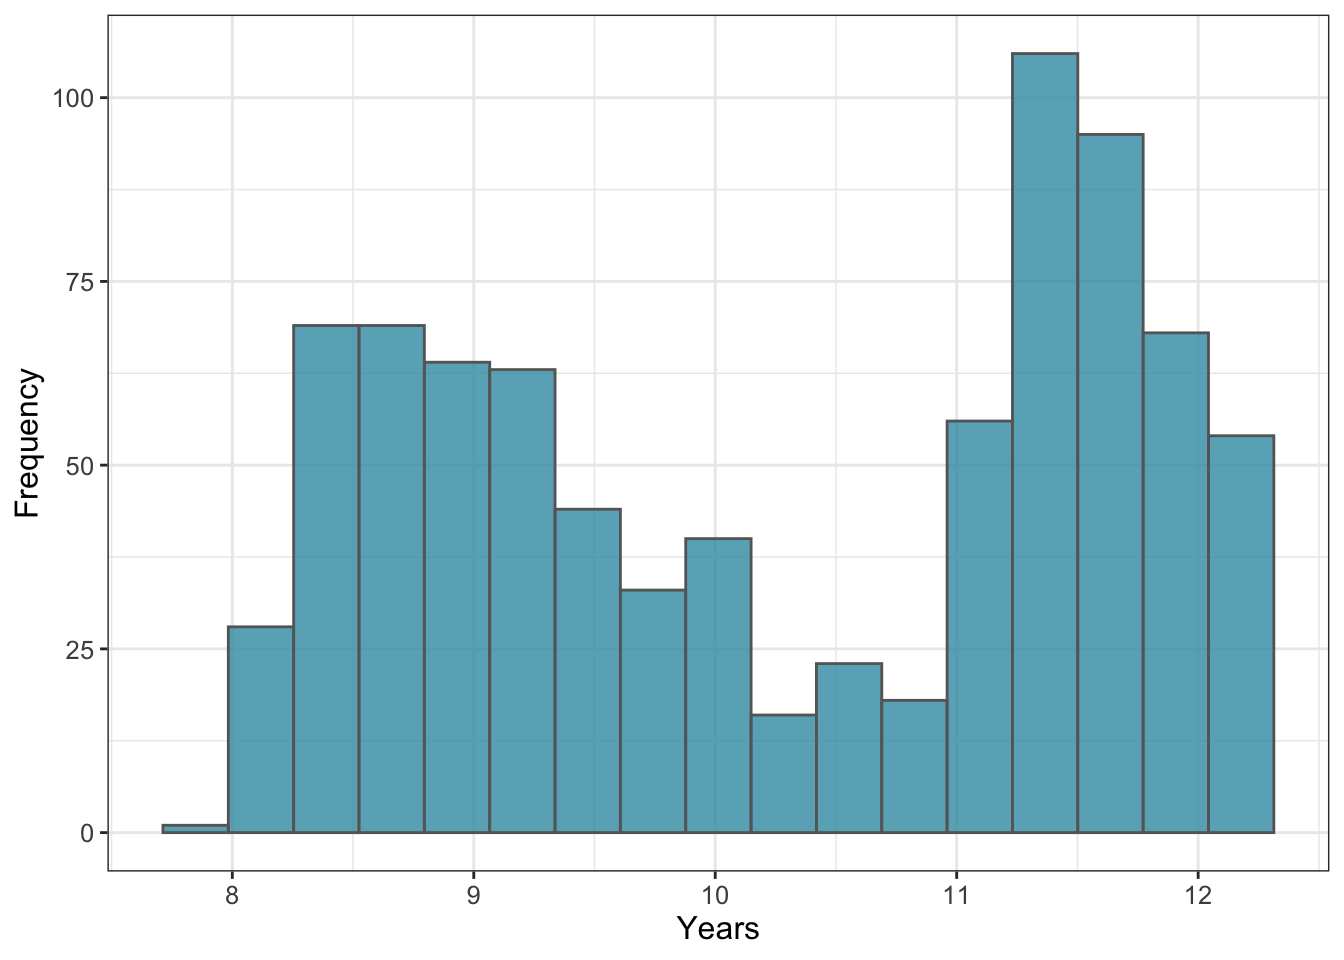
\includegraphics{attachment-bayes-factor_files/figure-latex/plot-age-1} 

}

\caption{Participants age distribution ($n_{subj} = 847$)}\label{fig:plot-age}
\end{figure}

\hypertarget{attachment-styles}{%
\section{Attachment Styles}\label{attachment-styles}}

Attachment towards the mother and the father was measured separately using the brief Experiences in Close Relationships Scale - Revised Child Version \citep[ECR-RC,][]{Brenning2014ThePQ, marciBriefExperiencesClose2019} completed by the children. Four main attachment styles have been recognized in the literature according to thee levels of \emph{anxiety} and \emph{avoidance}:

\begin{itemize}
\tightlist
\item
  \textbf{Secure Attachment -} children with low levels of anxiety and avoidance.
\item
  \textbf{Anxious Attachment -} children characterized by high levels of anxiety.
\item
  \textbf{Avoidant Attachment -} children characterized by high levels of avoidance.
\item
  \textbf{Fearful Attachment -} children with high levels of anxiety and avoidance.
\end{itemize}

To identify children's attachment styles towards the mother and towards the father, we conduct two separate cluster analyses. Clusters are obtained using the function \texttt{hclust()} (with argument \texttt{method="ward.D"}) considering \emph{Euclidean} distances between participants responses to the ECR items.

\hypertarget{mother-cluster-analysis}{%
\subsection{Mother Cluster Analysis}\label{mother-cluster-analysis}}

Regarding mother attachment, 4 groups are selected from the cluster analysis results (see Figure\textasciitilde\ref{fig:plot-cluster-mother}).

\begin{figure}

{\centering 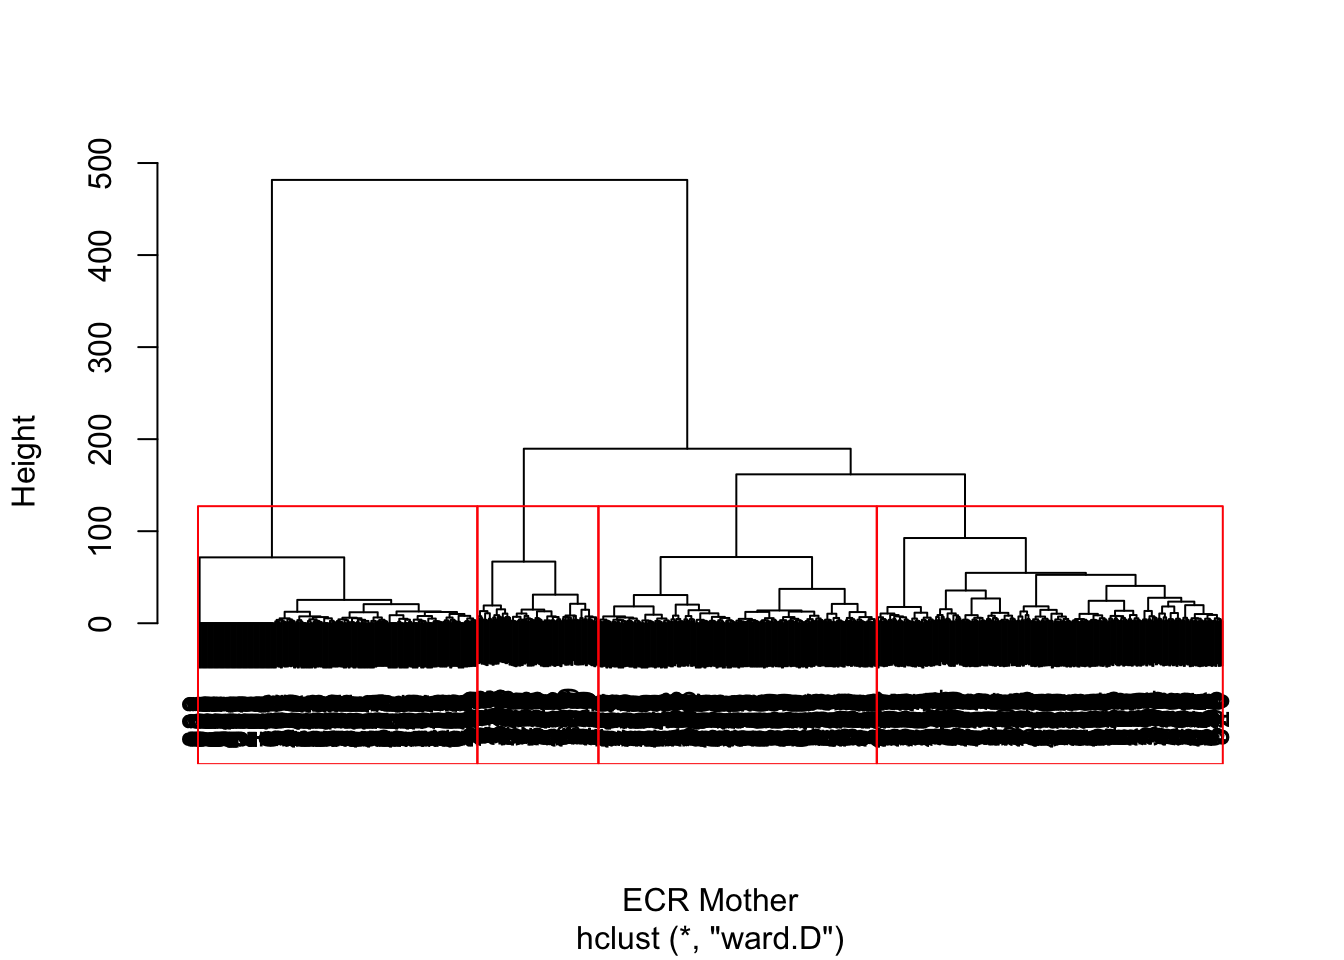
\includegraphics{attachment-bayes-factor_files/figure-latex/plot-cluster-mother-1} 

}

\caption{Mother attachment cluster dendrogram ($n_{subj} = 847$).}\label{fig:plot-cluster-mother}
\end{figure}

In Figure\textasciitilde\ref{fig:plot-scores-mother}, Anxiety (``\emph{Anx}'') and Avoidance (``\emph{Av}'') scores are presented according to mother attachment styles. The frequencies of mother attachment styles according to gender are reported in Table\textasciitilde\ref{tab:table-cluster-mother}.

\begin{figure}

{\centering 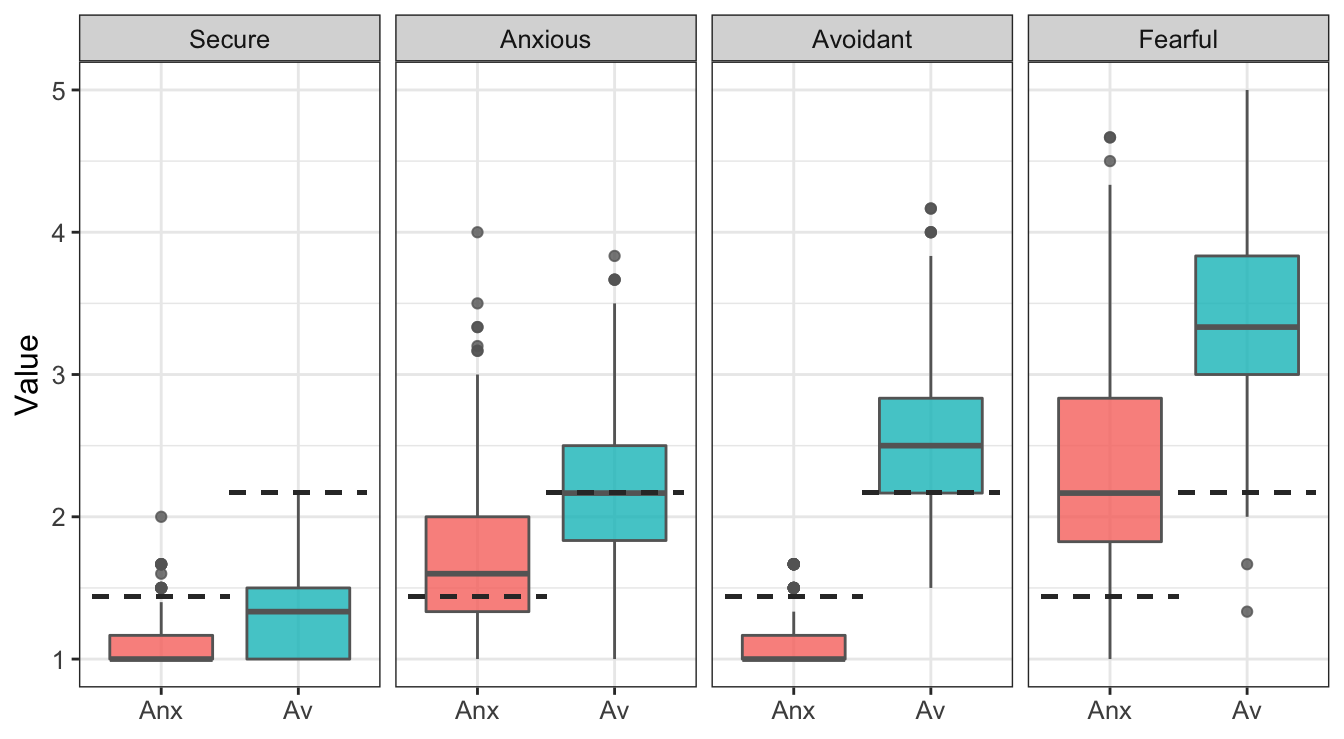
\includegraphics{attachment-bayes-factor_files/figure-latex/plot-scores-mother-1} 

}

\caption{Anxiety (“Anx”) and Avoidance (“Av”) scores according to mother attachment styles. Dashed lines represents overall average values ($n_{subj} = 847$).}\label{fig:plot-scores-mother}
\end{figure}

\begin{table}[!h]

\caption{\label{tab:table-cluster-mother}Mother attachment styles by gender ($n_{subj} = 847$).}
\centering
\begin{tabular}[t]{>{}rcccc}
\toprule
\multicolumn{1}{c}{\textbf{ }} & \multicolumn{4}{c}{\textbf{Attachment Style}} \\
\cmidrule(l{3pt}r{3pt}){2-5}
\textbf{Gender} & \textbf{Secure} & \textbf{Anxious} & \textbf{Avoidant} & \textbf{Fearful}\\
\midrule
\textbf{Females} & 132 (16\%) & 131 (15\%) & 111 (13\%) & 55 ( 6\%)\\
\textbf{Males} & 99 (12\%) & 155 (18\%) & 119 (14\%) & 45 ( 5\%)\\
\textbf{Total} & 231 (27\%) & 286 (34\%) & 230 (27\%) & 100 (12\%)\\
\bottomrule
\end{tabular}
\end{table}

Compared to the overall average values of anxiety and avoidance, we can observe that:

\begin{itemize}
\tightlist
\item
  \emph{Secure} children have lower levels of anxiety and avoidance
\item
  \emph{Anxious} children have higher levels of anxiety and about the average levels of avoidance
\item
  \emph{Avoidant} children have lower levels of anxiety and higher levels of avoidance
\item
  \emph{Fearful} children have higher levels of anxiety and avoidance
\end{itemize}

These results reflect the traditional definition of the four attachment styles.

\hypertarget{mclust-check}{%
\subsubsection*{Mclust Check}\label{mclust-check}}
\addcontentsline{toc}{subsubsection}{Mclust Check}

To evaluate if 4 clusters is an appropriate choice, we compare the BIC values of different model-based clustering options. To do that we use the function \texttt{mclustBIC()} from the \texttt{mclust} R-package \citep{scruccaMclustClusteringClassification2016}. BIC values of the best three model-based clusterings are reported below and overall results are presented in Figure\textasciitilde\ref{fig:plot-mclust-mother}. See \texttt{?mclustBIC()} help page for further information.

\begin{verbatim}
##   # Best model-based clustering for mother attachment
## Best BIC values:
##              EEV,6       EEV,7       EEV,9
## BIC      -23978.93 -24842.2954 -24969.9125
## BIC diff      0.00   -863.3681   -990.9852
\end{verbatim}

\begin{figure}

{\centering 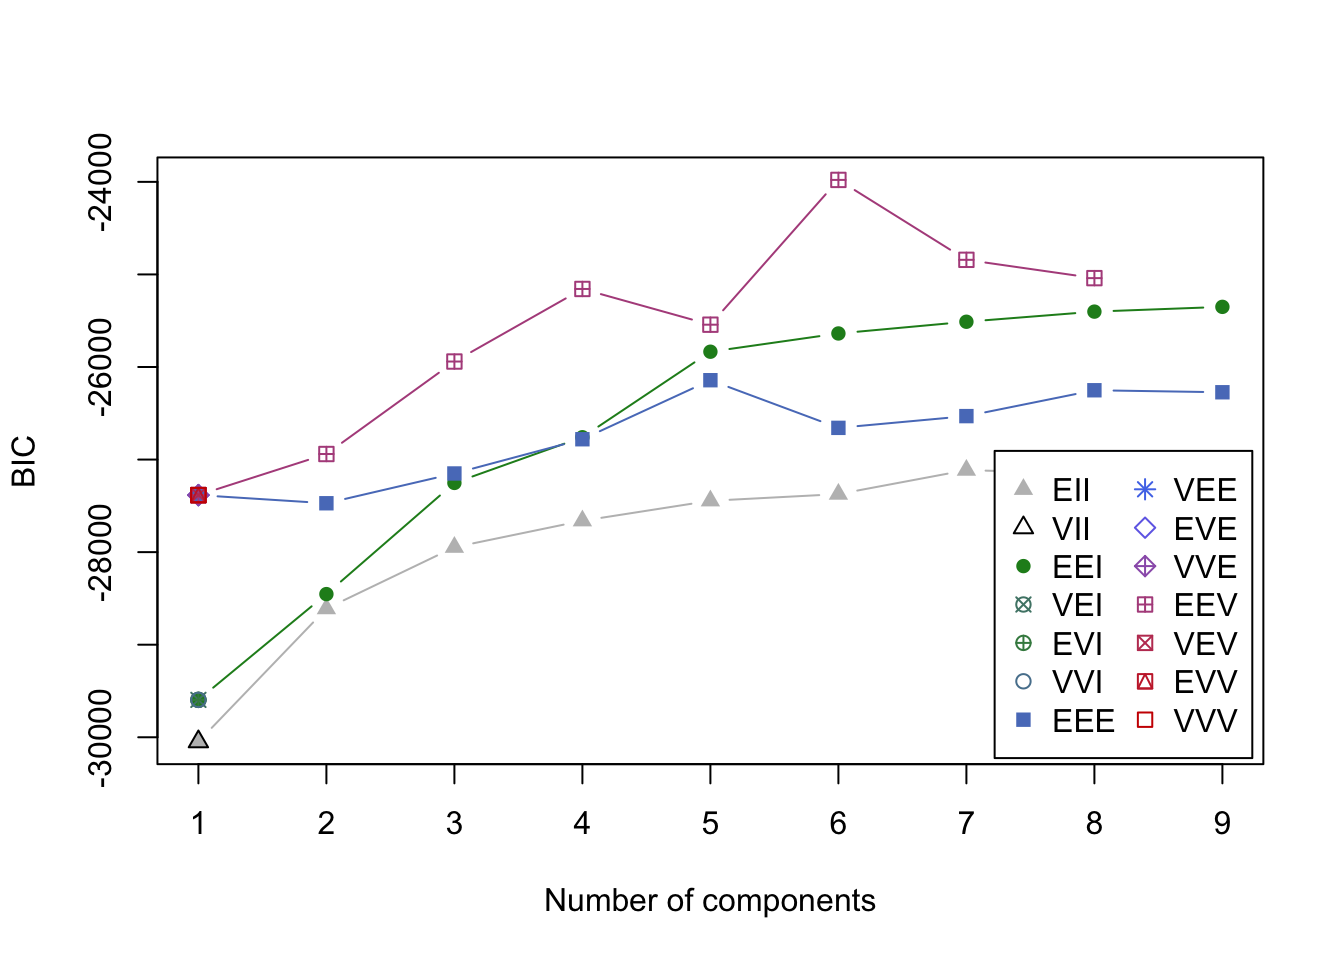
\includegraphics{attachment-bayes-factor_files/figure-latex/plot-mclust-mother-1} 

}

\caption{BIC values of different model-based clustering options. See '?mclustBIC()' help page for further information.}\label{fig:plot-mclust-mother}
\end{figure}

Results indicate the possible presence of a larger number of clusters. However, considering only 4 clusters seems to us the most reasonable choice. This is in line with attachment theory and general results in the literature. The important thing is that no smaller number of clusters provided better results than the division in 4 clusters.

\hypertarget{father-cluster-analysis}{%
\subsection{Father Cluster Analysis}\label{father-cluster-analysis}}

Regarding father attachment, 4 groups are selected from the cluster analysis results (see Figure\textasciitilde\ref{fig:plot-cluster-father}).

\begin{figure}

{\centering 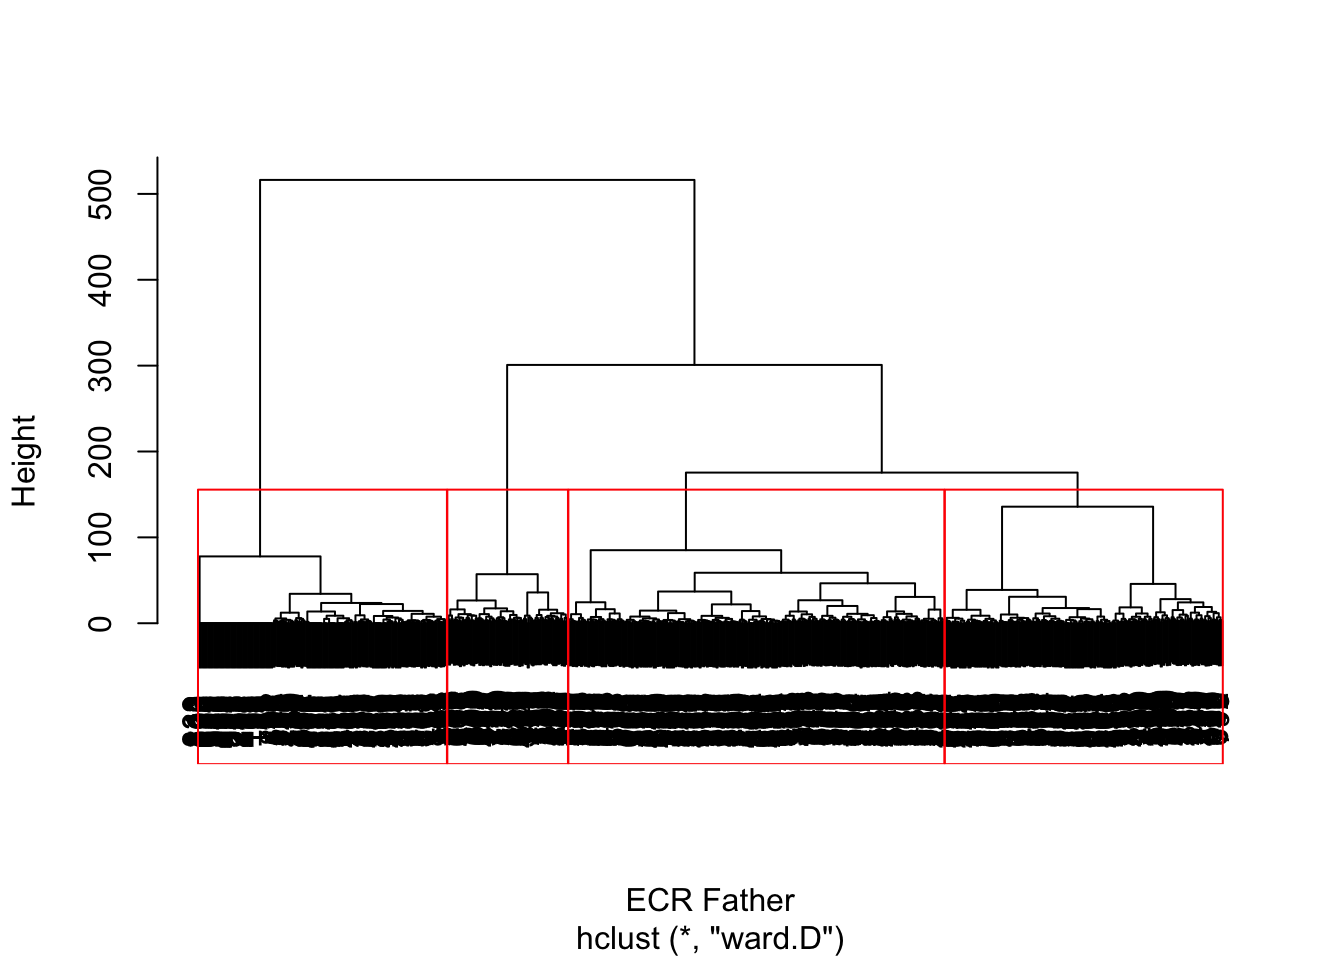
\includegraphics{attachment-bayes-factor_files/figure-latex/plot-cluster-father-1} 

}

\caption{Father attachment cluster dendrogram ($n_{subj} = 847$).}\label{fig:plot-cluster-father}
\end{figure}

In Figure\textasciitilde\ref{fig:plot-scores-father}, Anxiety (``\emph{Anx}'') and Avoidance (``\emph{Av}'') scores are presented according to father attachment styles. The frequencies of father attachment styles according to gender are reported in Table\textasciitilde\ref{tab:table-cluster-father}.

\begin{figure}

{\centering 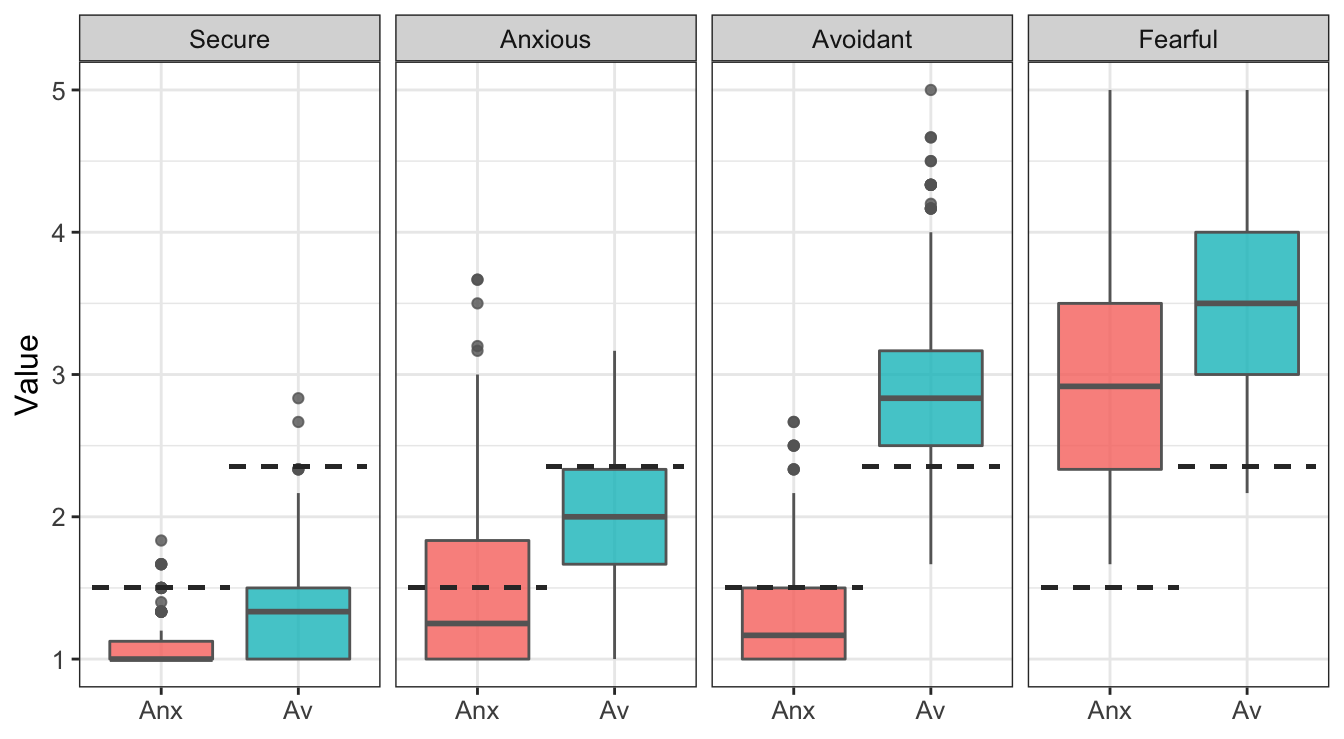
\includegraphics{attachment-bayes-factor_files/figure-latex/plot-scores-father-1} 

}

\caption{Anxiety (“Anx”) and Avoidance (“Av”) scores according to father attachment styles. Dashed lines represents overall average values ($n_{subj} = 847$).}\label{fig:plot-scores-father}
\end{figure}

\begin{table}[!h]

\caption{\label{tab:table-cluster-father}Father attachment styles by gender ($n_{subj} = 847$).}
\centering
\begin{tabular}[t]{>{}rcccc}
\toprule
\multicolumn{1}{c}{\textbf{ }} & \multicolumn{4}{c}{\textbf{Attachment Style}} \\
\cmidrule(l{3pt}r{3pt}){2-5}
\textbf{Gender} & \textbf{Secure} & \textbf{Anxious} & \textbf{Avoidant} & \textbf{Fearful}\\
\midrule
\textbf{Females} & 99 (12\%) & 104 (12\%) & 163 (19\%) & 63 ( 7\%)\\
\textbf{Males} & 107 (13\%) & 126 (15\%) & 148 (17\%) & 37 ( 4\%)\\
\textbf{Total} & 206 (24\%) & 230 (27\%) & 311 (37\%) & 100 (12\%)\\
\bottomrule
\end{tabular}
\end{table}

Compared to the overall average values of anxiety and avoidance, we can observe that:

\begin{itemize}
\tightlist
\item
  \emph{Secure} children have lower levels of anxiety and avoidance
\item
  \emph{Anxious} children have lower levels of anxiety and avoidance
\item
  \emph{Avoidant} children have lower levels of anxiety and higher levels of avoidance
\item
  \emph{Fearful} children have higher levels of anxiety and avoidance
\end{itemize}

These results are not as good as in the mother attachment classification, but they are still reasonable.

\hypertarget{mclust-check-1}{%
\subsubsection*{Mclust Check}\label{mclust-check-1}}
\addcontentsline{toc}{subsubsection}{Mclust Check}

To evaluate if 4 clusters is an appropriate choice, we compare the BIC values of different model-based clustering options as before. BIC values of the best three model-based clusterings are reported below and overall results are presented in Figure\textasciitilde\ref{fig:plot-mclust-father}.

\begin{verbatim}
##   # Best model-based clustering for father attachment
## Best BIC values:
##              EEV,9       EEV,5       EEV,8
## BIC      -25351.48 -25905.1973 -25979.1378
## BIC diff      0.00   -553.7208   -627.6613
\end{verbatim}

\begin{figure}

{\centering 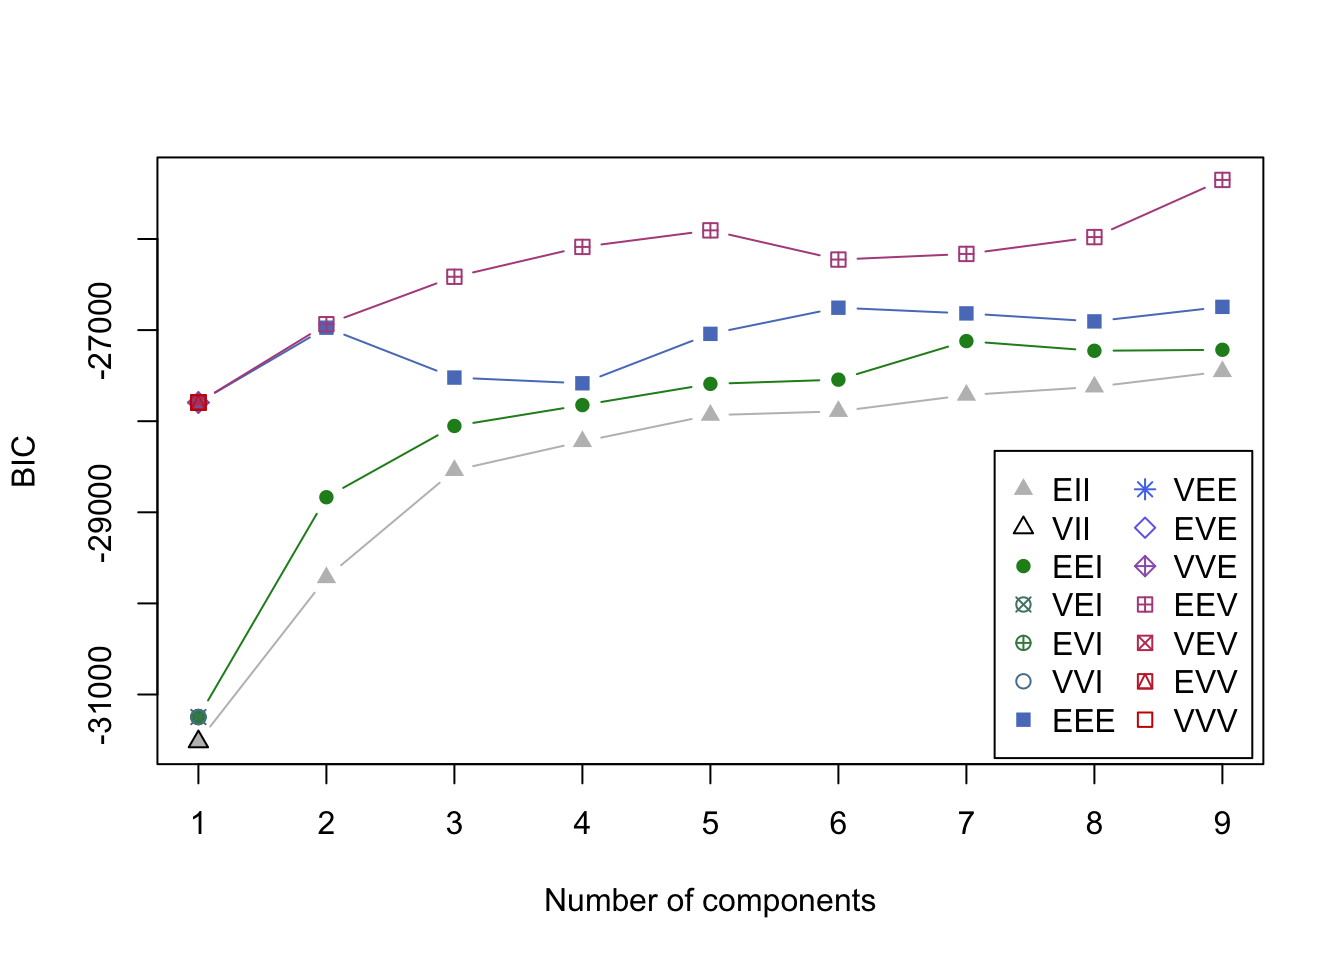
\includegraphics{attachment-bayes-factor_files/figure-latex/plot-mclust-father-1} 

}

\caption{BIC values of different model-based clustering options. See '?mclustBIC()' help page for further information.}\label{fig:plot-mclust-father}
\end{figure}

As for the mother, results indicate the possible presence of a larger number of clusters. However, considering only 4 clusters seems to us the most reasonable choice for the same reasons as before.

\hypertarget{mother-and-father}{%
\subsection{Mother and Father}\label{mother-and-father}}

The frequencies of mother attachment and father attachment styles are reported in Table\textasciitilde\ref{tab:table-cluster-mother-father}.

\begin{table}[!h]

\caption{\label{tab:table-cluster-mother-father}Mother attachment and father attachemtn styles ($n_{subj} = 847$).}
\centering
\begin{tabular}[t]{>{}rcccc}
\toprule
\multicolumn{1}{c}{\textbf{ }} & \multicolumn{4}{c}{\textbf{Father Attachment}} \\
\cmidrule(l{3pt}r{3pt}){2-5}
\textbf{Mother Attachment} & \textbf{Secure} & \textbf{Anxious} & \textbf{Avoidant} & \textbf{Fearful}\\
\midrule
\textbf{Secure} & 125 (15\%) & 49 ( 6\%) & 49 ( 6\%) & 8 (1\%)\\
\textbf{Anxious} & 51 ( 6\%) & 100 (12\%) & 98 (12\%) & 37 (4\%)\\
\textbf{Avoidant} & 25 ( 3\%) & 67 ( 8\%) & 126 (15\%) & 12 (1\%)\\
\textbf{Fearful} & 5 ( 1\%) & 14 ( 2\%) & 38 ( 4\%) & 43 (5\%)\\
\bottomrule
\end{tabular}
\end{table}

We can observe how values on the diagonal (same attachment styles towards both parents) tend to be larger than others.

\hypertarget{children-outcomes}{%
\section{Children Outcomes}\label{children-outcomes}}

Children's social-emotional development was measured using the Strength and Difficulties Questionnaire \citep[SDQ,][]{goodmanWhenUseBroader2010} completed by the teachers. Separate scores for externalizing and internalizing problems were obtained as the sum of the questionnaire items.

\hypertarget{externalizing-problems-1}{%
\subsection{Externalizing Problems}\label{externalizing-problems-1}}

Participants externalizing problems mean is 3.35 (SD = 3.91). The participants' externalizing problems summary statistics are reported below and the distribution is presented in Figure\textasciitilde\ref{fig:plot-externalizing-dist}.

\begin{verbatim}
##   # Externalizing problems summary statistics
##    Min. 1st Qu.  Median    Mean 3rd Qu.    Max. 
##   0.000   0.000   2.000   3.349   6.000  18.000
\end{verbatim}

\begin{figure}

{\centering 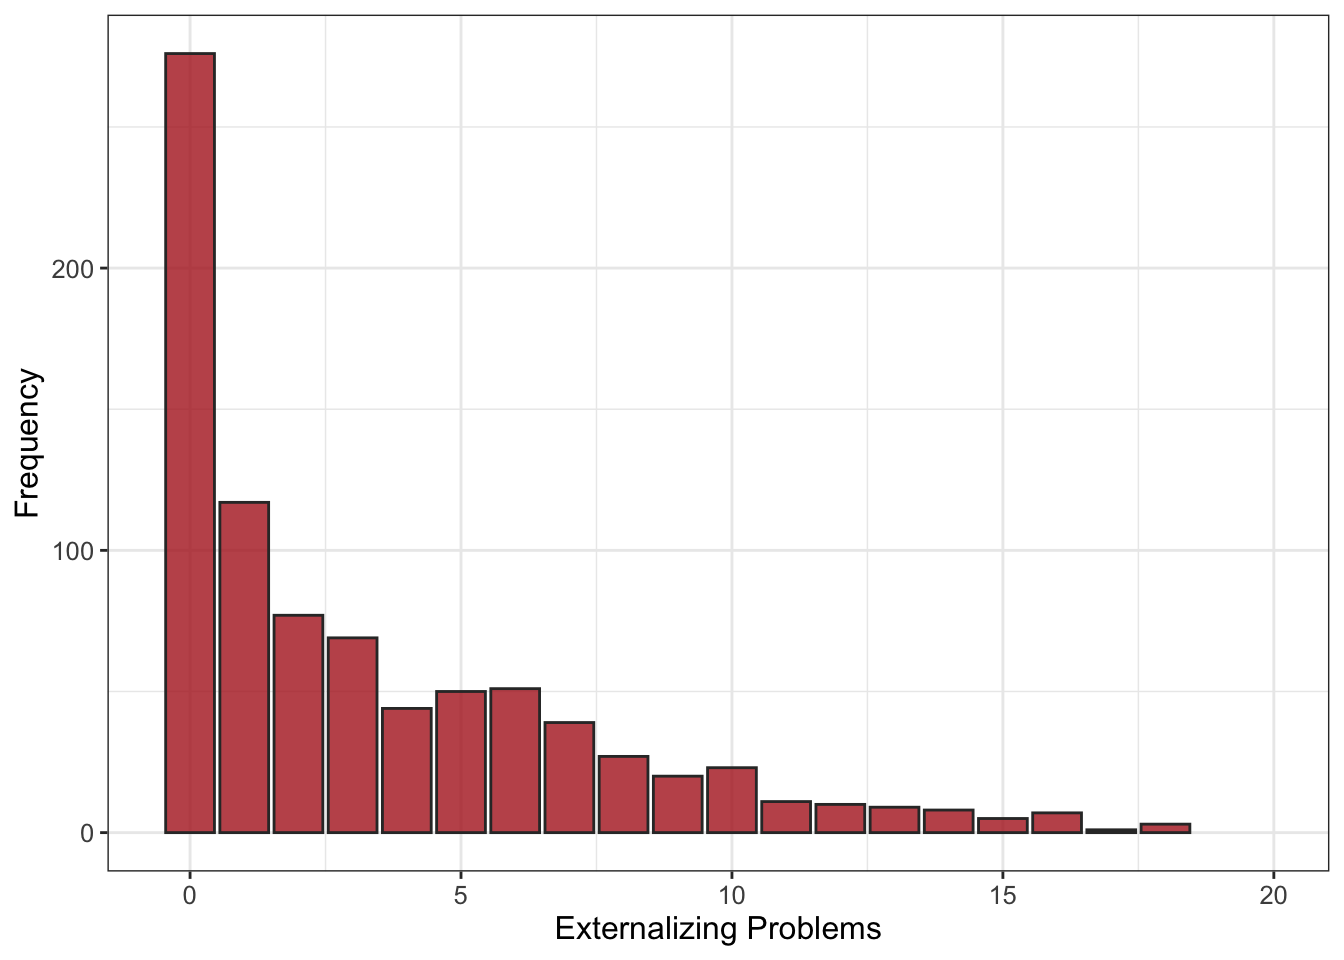
\includegraphics{attachment-bayes-factor_files/figure-latex/plot-externalizing-dist-1} 

}

\caption{Participants externalizing problems distribution ($n_{subj} = 847$)}\label{fig:plot-externalizing-dist}
\end{figure}

Overall, externalizing problems are low. This is expected as the sample is not clinical. Externalizing problems according to attachment styles are reported in Table\textasciitilde\ref{tab:table-cluster-ext}.

\begin{table}[!h]

\caption{\label{tab:table-cluster-ext}Externalizing problems according to attachment styles ($n_{subj} = 847$).}
\centering
\resizebox{\linewidth}{!}{
\begin{tabular}[t]{>{}rcccccccc}
\toprule
\multicolumn{1}{c}{\textbf{ }} & \multicolumn{8}{c}{\textbf{Father Attachment}} \\
\cmidrule(l{3pt}r{3pt}){2-9}
\multicolumn{1}{c}{\textbf{ }} & \multicolumn{2}{c}{\textbf{Secure}} & \multicolumn{2}{c}{\textbf{Anxious}} & \multicolumn{2}{c}{\textbf{Avoidant}} & \multicolumn{2}{c}{\textbf{Fearful}} \\
\cmidrule(l{3pt}r{3pt}){2-3} \cmidrule(l{3pt}r{3pt}){4-5} \cmidrule(l{3pt}r{3pt}){6-7} \cmidrule(l{3pt}r{3pt}){8-9}
\textbf{Mother Attachment} & \textbf{Mean (SD)} & \textbf{Median} & \textbf{Mean (SD)} & \textbf{Median} & \textbf{Mean (SD)} & \textbf{Median} & \textbf{Mean (SD)} & \textbf{Median}\\
\midrule
\textbf{Secure} & 2.63 (3.57) & 1.0 & 3.45 (4.48) & 2.0 & 1.61 (2.13) & 1.0 & 2.88 (3.44) & 2.0\\
\textbf{Anxious} & 3.69 (4.07) & 2.0 & 3.01 (3.61) & 2.0 & 3.32 (4.12) & 2.0 & 4.05 (3.61) & 3.0\\
\textbf{Avoidant} & 2.84 (3.34) & 1.0 & 3.31 (3.65) & 2.0 & 3.71 (4.19) & 2.0 & 3.75 (4.81) & 1.0\\
\textbf{Fearful} & 7.60 (4.04) & 8.0 & 4.64 (3.84) & 4.5 & 4.76 (4.67) & 3.0 & 4.26 (4.07) & 4.0\\
\bottomrule
\end{tabular}}
\end{table}

\hypertarget{internalizing-problems-1}{%
\subsection{Internalizing Problems}\label{internalizing-problems-1}}

Participants internalizing problems mean is 2.96 (SD = 3.14). The participants internalizing problems summary statistics are reported below and the distribution is presented in Figure\textasciitilde\ref{fig:plot-internalizing-dist}.

\begin{verbatim}
##   # Internalizing problems summary statistics
##    Min. 1st Qu.  Median    Mean 3rd Qu.    Max. 
##   0.000   0.000   2.000   2.955   4.000  18.000
\end{verbatim}

\begin{figure}

{\centering 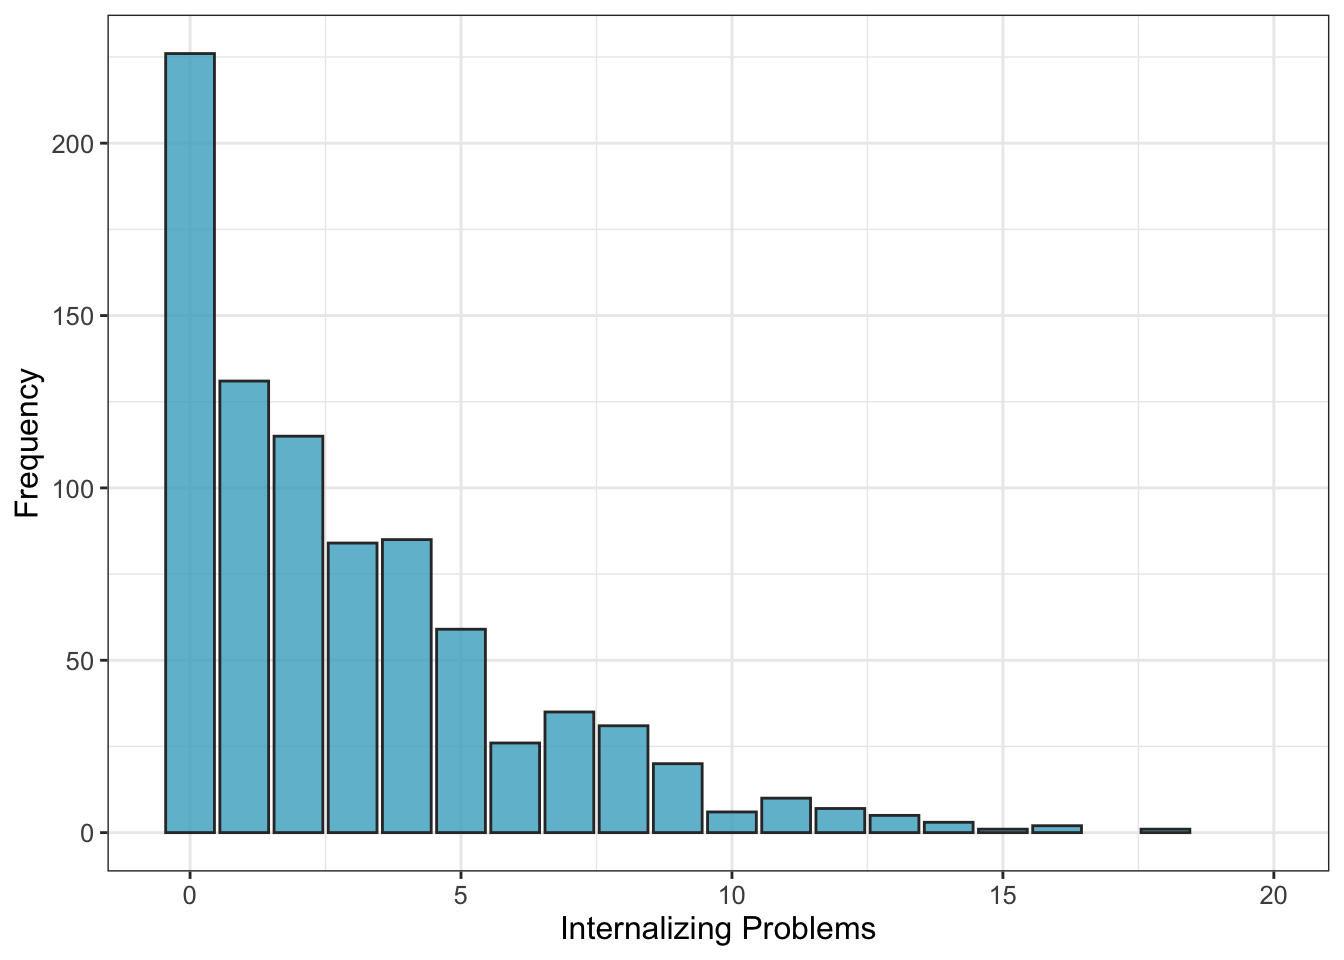
\includegraphics{attachment-bayes-factor_files/figure-latex/plot-internalizing-dist-1} 

}

\caption{Participants internalizing problems distribution ($n_{subj} = 847$)}\label{fig:plot-internalizing-dist}
\end{figure}

Overall, internalizing problems are low. Again, this is expected as the sample is not clinical. Internalizing problems according to attachment styles are reported in Table\textasciitilde\ref{tab:table-cluster-int}.

\begin{table}[!h]

\caption{\label{tab:table-cluster-int}Internalizing problems according to attachment styles ($n_{subj} = 847$).}
\centering
\resizebox{\linewidth}{!}{
\begin{tabular}[t]{>{}rcccccccc}
\toprule
\multicolumn{1}{c}{\textbf{ }} & \multicolumn{8}{c}{\textbf{Father Attachment}} \\
\cmidrule(l{3pt}r{3pt}){2-9}
\multicolumn{1}{c}{\textbf{ }} & \multicolumn{2}{c}{\textbf{Secure}} & \multicolumn{2}{c}{\textbf{Anxious}} & \multicolumn{2}{c}{\textbf{Avoidant}} & \multicolumn{2}{c}{\textbf{Fearful}} \\
\cmidrule(l{3pt}r{3pt}){2-3} \cmidrule(l{3pt}r{3pt}){4-5} \cmidrule(l{3pt}r{3pt}){6-7} \cmidrule(l{3pt}r{3pt}){8-9}
\textbf{Mother Attachment} & \textbf{Mean (SD)} & \textbf{Median} & \textbf{Mean (SD)} & \textbf{Median} & \textbf{Mean (SD)} & \textbf{Median} & \textbf{Mean (SD)} & \textbf{Median}\\
\midrule
\textbf{Secure} & 2.29 (2.64) & 1.0 & 2.63 (2.75) & 2.0 & 2.67 (2.75) & 3.0 & 3.62 (3.46) & 3.0\\
\textbf{Anxious} & 3.29 (3.48) & 2.0 & 3.15 (3.09) & 2.0 & 3.28 (3.72) & 2.0 & 3.11 (3.81) & 2.0\\
\textbf{Avoidant} & 1.88 (2.28) & 1.0 & 2.99 (3.22) & 2.0 & 2.65 (2.86) & 2.0 & 4.08 (3.78) & 3.5\\
\textbf{Fearful} & 4.40 (3.65) & 4.0 & 2.07 (1.69) & 2.0 & 3.68 (3.68) & 3.0 & 4.37 (3.12) & 4.0\\
\bottomrule
\end{tabular}}
\end{table}

\hypertarget{part-externalizing-problems}{%
\part*{Externalizing Problems}\label{part-externalizing-problems}}
\addcontentsline{toc}{part}{Externalizing Problems}

\hypertarget{model-choice-ext}{%
\chapter{Models Family Choice}\label{model-choice-ext}}

In this chapter, we discuss the appropriate models' family to take into account data characteristics.

\hypertarget{negative-binomial}{%
\section{Negative Binomial}\label{negative-binomial}}

Externalizing problems are computed as the sum of 10 items of the SDQ, obtaining discrete scores that range from 0 to 20. Thus, we should use appropriate discrete distribution such as the \emph{Poisson} distribution or the \emph{Negative Binomial}. In the Poisson distribution mean and variance are defined according to the same parameter \(\lambda\). On the contrary, Negative Binomial has an extra parameter to adjust the variance allowing more flexibility. Considering data distribution (see Figure\textasciitilde\ref{fig:plot-externalizing-dist}), we can observe that data have high dispersion with a long right tail. In this case, the Poisson distribution would be a poor choice and we prefer Negative Binomial instead.

Again, considering data distribution (see Figure\textasciitilde\ref{fig:plot-externalizing-dist}), we can observe a high peak of values at zero. Remember that this is not a clinical sample, thus it is expected that the majority of children have no problems or really few problems. We could question ourselves, however, whether a \emph{Zero-Inflated} model may be appropriate

\hypertarget{zero-inflated-negative-binomial}{%
\section{Zero Inflated Negative Binomial}\label{zero-inflated-negative-binomial}}

To evaluate the presence of zero inflation in our data, we compare the number of observed zeros and expected zeros in a Negative Binomial mixed-effects model. We consider in the model the role of gender and the interaction between mother attachment and father attachment. Moreover, we consider the children's classroom ID as a random effect to account for teachers' different ability to evaluate children's problems. Using R formula syntax, we have

\begin{Shaded}
\begin{Highlighting}[]
\CommentTok{\# model formula}
\NormalTok{externalizing\_sum }\SpecialCharTok{\textasciitilde{}}\NormalTok{ gender }\SpecialCharTok{+}\NormalTok{ mother }\SpecialCharTok{*}\NormalTok{ father }\SpecialCharTok{+}\NormalTok{ (}\DecValTok{1}\SpecialCharTok{|}\NormalTok{ID\_class)}
\end{Highlighting}
\end{Shaded}

The model is fitted using the function \texttt{glmmTMB()} from the \texttt{glmmTMB} R-package \citep{brooksGlmmTMBBalancesSpeed2017}. Next, we compare the number of observed zero and expected zeros using an adapted version of the function \texttt{check\_zeroinflation()} from the R-package \texttt{performance} \citep{ludeckePerformancePackageAssessment2021} that solves a small bug (see issue \url{https://github.com/easystats/performance/issues/367}).

\begin{Shaded}
\begin{Highlighting}[]
\FunctionTok{my\_check\_zeroinflation}\NormalTok{(fit\_ext\_nb)}
\DocumentationTok{\#\# \# Check for zero{-}inflation}
\DocumentationTok{\#\# }
\DocumentationTok{\#\#    Observed zeros: 276}
\DocumentationTok{\#\#   Predicted zeros: 245}
\DocumentationTok{\#\#             Ratio: 0.89}
\DocumentationTok{\#\# Model is underfitting zeros (probable zero{-}inflation).}
\end{Highlighting}
\end{Shaded}

Results indicate that the model is slightly under-fitting the number of zeros. Now, we can try to fit a \emph{Zero Inflated Negative Binomial} (ZINB) model and compare the performance of the two models. ZINB models are defined as
\[
y_{ij} \sim ZINB(p_{ij}, \mu_{ij}, \phi),
\]
where \(p_{ij}\) is the probability of an observation \(y_{ij}\) being an extra zero (i.e., a zero not coming from the Negative Binomial distribution) and \(1-p_{ij}\) indicates the probability of a given observation \(y_{ij}\) being generated form a Negative Binomial distribution with mean \(\mu_{ij}\) and variance \(\sigma_{ij}^2 = \mu_{ij} + \frac{\mu_{ij}^2}{\phi}\). Moreover, we have that
\[
p_{ij} = \text{logit}^{-1}(X_i^T\beta_p+ Z_j^Tu_p),\\
\mu_{ij} = \text{exp}(X_i^T\beta_{\mu}+ Z_j^Tu_{\mu}).
\]
That is, both \(p\) and \(\mu\) are modelled separately according to (possibly) different variables. In our case, we consider only the role of gender for \(p\) (i.e., the probability of having externalizing problems depends on gender), whereas for \(\mu\) we also consider the interaction between mother attachment and father attachment. In both cases, we consider the children's classroom ID as a random effect (teachers may differ in the ability to detect children's problems and quantify them). Using R formula syntax, we have

\begin{Shaded}
\begin{Highlighting}[]
\CommentTok{\# formula for p}
\NormalTok{p }\SpecialCharTok{\textasciitilde{}}\NormalTok{ gender }\SpecialCharTok{+}\NormalTok{ (}\DecValTok{1}\SpecialCharTok{|}\NormalTok{ID\_class)}

\CommentTok{\# formula for mu}
\NormalTok{mu }\SpecialCharTok{\textasciitilde{}}\NormalTok{ gender }\SpecialCharTok{+}\NormalTok{ mother }\SpecialCharTok{*}\NormalTok{ father }\SpecialCharTok{+}\NormalTok{ (}\DecValTok{1}\SpecialCharTok{|}\NormalTok{ID\_class)}
\end{Highlighting}
\end{Shaded}

The ZINB model is fitted using the function \texttt{glmmTMB()}. To compare the ZINB model and the Negative Binomial model we conduct an analysis of \emph{Deviance}. Note that, in the case of generalized linear models (GLM), the deviance is the corresponding of the residual variance used in the traditional ANOVA in the case of linear models.

\begin{Shaded}
\begin{Highlighting}[]
\FunctionTok{anova}\NormalTok{(fit\_ext\_nb, fit\_ext\_zinb)}
\DocumentationTok{\#\# Data: data\_cluster}
\DocumentationTok{\#\# Models:}
\DocumentationTok{\#\# fit\_ext\_nb: externalizing\_sum \textasciitilde{} gender + mother * father + (1 | ID\_class), zi=\textasciitilde{}0, disp=\textasciitilde{}1}
\DocumentationTok{\#\# fit\_ext\_zinb: externalizing\_sum \textasciitilde{} gender + mother * father + (1 | ID\_class), zi=\textasciitilde{}gender + (1 | ID\_class), disp=\textasciitilde{}1}
\DocumentationTok{\#\#              Df    AIC    BIC  logLik deviance  Chisq Chi Df Pr(\textgreater{}Chisq)    }
\DocumentationTok{\#\# fit\_ext\_nb   19 3910.1 4000.2 {-}1936.1   3872.1                             }
\DocumentationTok{\#\# fit\_ext\_zinb 22 3867.6 3971.9 {-}1911.8   3823.6 48.556      3  1.622e{-}10 ***}
\DocumentationTok{\#\# {-}{-}{-}}
\DocumentationTok{\#\# Signif. codes:  0 \textquotesingle{}***\textquotesingle{} 0.001 \textquotesingle{}**\textquotesingle{} 0.01 \textquotesingle{}*\textquotesingle{} 0.05 \textquotesingle{}.\textquotesingle{} 0.1 \textquotesingle{} \textquotesingle{} 1}
\end{Highlighting}
\end{Shaded}

Overall, results indicate that the ZINB model performs better than the Negative Binomial model. Thus, in the following analyses, we decide to use ZINB models.

\hypertarget{nhst-ext}{%
\chapter{NHST}\label{nhst-ext}}

Following the traditional NHST approach, we consider the model previously defined that includes all effects of interest. That is the gender effect and the interaction between mother attachment and father attachment. Subsequently, we can run an analysis of deviance to evaluate the significance of the predictors using the function \texttt{Anova()} from the R-package \texttt{car} \citep{foxCompanionAppliedRegression2019}.

\begin{Shaded}
\begin{Highlighting}[]
\NormalTok{car}\SpecialCharTok{::}\FunctionTok{Anova}\NormalTok{(fit\_ext\_zinb)}
\DocumentationTok{\#\# Analysis of Deviance Table (Type II Wald chisquare tests)}
\DocumentationTok{\#\# }
\DocumentationTok{\#\# Response: externalizing\_sum}
\DocumentationTok{\#\#                 Chisq Df Pr(\textgreater{}Chisq)    }
\DocumentationTok{\#\# gender        15.2947  1  9.197e{-}05 ***}
\DocumentationTok{\#\# mother        15.6195  3   0.001357 ** }
\DocumentationTok{\#\# father         1.1006  3   0.776938    }
\DocumentationTok{\#\# mother:father  8.9096  9   0.445657    }
\DocumentationTok{\#\# {-}{-}{-}}
\DocumentationTok{\#\# Signif. codes:  0 \textquotesingle{}***\textquotesingle{} 0.001 \textquotesingle{}**\textquotesingle{} 0.01 \textquotesingle{}*\textquotesingle{} 0.05 \textquotesingle{}.\textquotesingle{} 0.1 \textquotesingle{} \textquotesingle{} 1}
\end{Highlighting}
\end{Shaded}

Results indicate a statistically significant effect of gender and mother attachment. On the contrary, the interaction and father attachment are not significant. The model summary is reported below.

\begin{Shaded}
\begin{Highlighting}[]
\FunctionTok{summary}\NormalTok{(fit\_ext\_zinb)}
\DocumentationTok{\#\#  Family: nbinom2  ( log )}
\DocumentationTok{\#\# Formula:          externalizing\_sum \textasciitilde{} gender + mother * father + (1 | ID\_class)}
\DocumentationTok{\#\# Zero inflation:                     \textasciitilde{}gender + (1 | ID\_class)}
\DocumentationTok{\#\# Data: data\_cluster}
\DocumentationTok{\#\# }
\DocumentationTok{\#\#      AIC      BIC   logLik deviance df.resid }
\DocumentationTok{\#\#   3867.6   3971.9  {-}1911.8   3823.6      825 }
\DocumentationTok{\#\# }
\DocumentationTok{\#\# Random effects:}
\DocumentationTok{\#\# }
\DocumentationTok{\#\# Conditional model:}
\DocumentationTok{\#\#  Groups   Name        Variance Std.Dev.}
\DocumentationTok{\#\#  ID\_class (Intercept) 0.08132  0.2852  }
\DocumentationTok{\#\# Number of obs: 847, groups:  ID\_class, 50}
\DocumentationTok{\#\# }
\DocumentationTok{\#\# Zero{-}inflation model:}
\DocumentationTok{\#\#  Groups   Name        Variance Std.Dev.}
\DocumentationTok{\#\#  ID\_class (Intercept) 0.7669   0.8757  }
\DocumentationTok{\#\# Number of obs: 847, groups:  ID\_class, 50}
\DocumentationTok{\#\# }
\DocumentationTok{\#\# Dispersion parameter for nbinom2 family (): 1.86 }
\DocumentationTok{\#\# }
\DocumentationTok{\#\# Conditional model:}
\DocumentationTok{\#\#                               Estimate Std. Error z value Pr(\textgreater{}|z|)    }
\DocumentationTok{\#\# (Intercept)                    1.01996    0.12814   7.960 1.72e{-}15 ***}
\DocumentationTok{\#\# genderM                        0.31556    0.08069   3.911 9.20e{-}05 ***}
\DocumentationTok{\#\# motherAnxious                  0.30735    0.18664   1.647   0.0996 .  }
\DocumentationTok{\#\# motherAvoidant                 0.14496    0.25509   0.568   0.5699    }
\DocumentationTok{\#\# motherFearful                  0.62950    0.39550   1.592   0.1115    }
\DocumentationTok{\#\# fatherAnxious                  0.21543    0.19156   1.125   0.2607    }
\DocumentationTok{\#\# fatherAvoidant                {-}0.46555    0.21138  {-}2.202   0.0276 *  }
\DocumentationTok{\#\# fatherFearful                  0.07138    0.41737   0.171   0.8642    }
\DocumentationTok{\#\# motherAnxious:fatherAnxious   {-}0.38346    0.26981  {-}1.421   0.1553    }
\DocumentationTok{\#\# motherAvoidant:fatherAnxious  {-}0.09675    0.33041  {-}0.293   0.7697    }
\DocumentationTok{\#\# motherFearful:fatherAnxious   {-}0.40811    0.49348  {-}0.827   0.4082    }
\DocumentationTok{\#\# motherAnxious:fatherAvoidant   0.34281    0.28290   1.212   0.2256    }
\DocumentationTok{\#\# motherAvoidant:fatherAvoidant  0.63111    0.32765   1.926   0.0541 .  }
\DocumentationTok{\#\# motherFearful:fatherAvoidant   0.34025    0.46490   0.732   0.4642    }
\DocumentationTok{\#\# motherAnxious:fatherFearful   {-}0.04630    0.47448  {-}0.098   0.9223    }
\DocumentationTok{\#\# motherAvoidant:fatherFearful   0.11794    0.56413   0.209   0.8344    }
\DocumentationTok{\#\# motherFearful:fatherFearful   {-}0.20316    0.58602  {-}0.347   0.7288    }
\DocumentationTok{\#\# {-}{-}{-}}
\DocumentationTok{\#\# Signif. codes:  0 \textquotesingle{}***\textquotesingle{} 0.001 \textquotesingle{}**\textquotesingle{} 0.01 \textquotesingle{}*\textquotesingle{} 0.05 \textquotesingle{}.\textquotesingle{} 0.1 \textquotesingle{} \textquotesingle{} 1}
\DocumentationTok{\#\# }
\DocumentationTok{\#\# Zero{-}inflation model:}
\DocumentationTok{\#\#             Estimate Std. Error z value Pr(\textgreater{}|z|)    }
\DocumentationTok{\#\# (Intercept)  {-}1.1239     0.2417   {-}4.65 3.32e{-}06 ***}
\DocumentationTok{\#\# genderM      {-}0.7145     0.2516   {-}2.84  0.00451 ** }
\DocumentationTok{\#\# {-}{-}{-}}
\DocumentationTok{\#\# Signif. codes:  0 \textquotesingle{}***\textquotesingle{} 0.001 \textquotesingle{}**\textquotesingle{} 0.01 \textquotesingle{}*\textquotesingle{} 0.05 \textquotesingle{}.\textquotesingle{} 0.1 \textquotesingle{} \textquotesingle{} 1}
\end{Highlighting}
\end{Shaded}

To evaluate the effect of gender and mother attachment, the marginal predicted values according to gender and mother attachment are presented separately in Figure\textasciitilde\ref{fig:plot-nhst-effects-ext}. Not that the marginal predicted values for gender are averaged over mother and father attachment effects. Whereas, the marginal predicted values for mother attachment are averaged over father attachment and gender effect.

\begin{figure}

{\centering 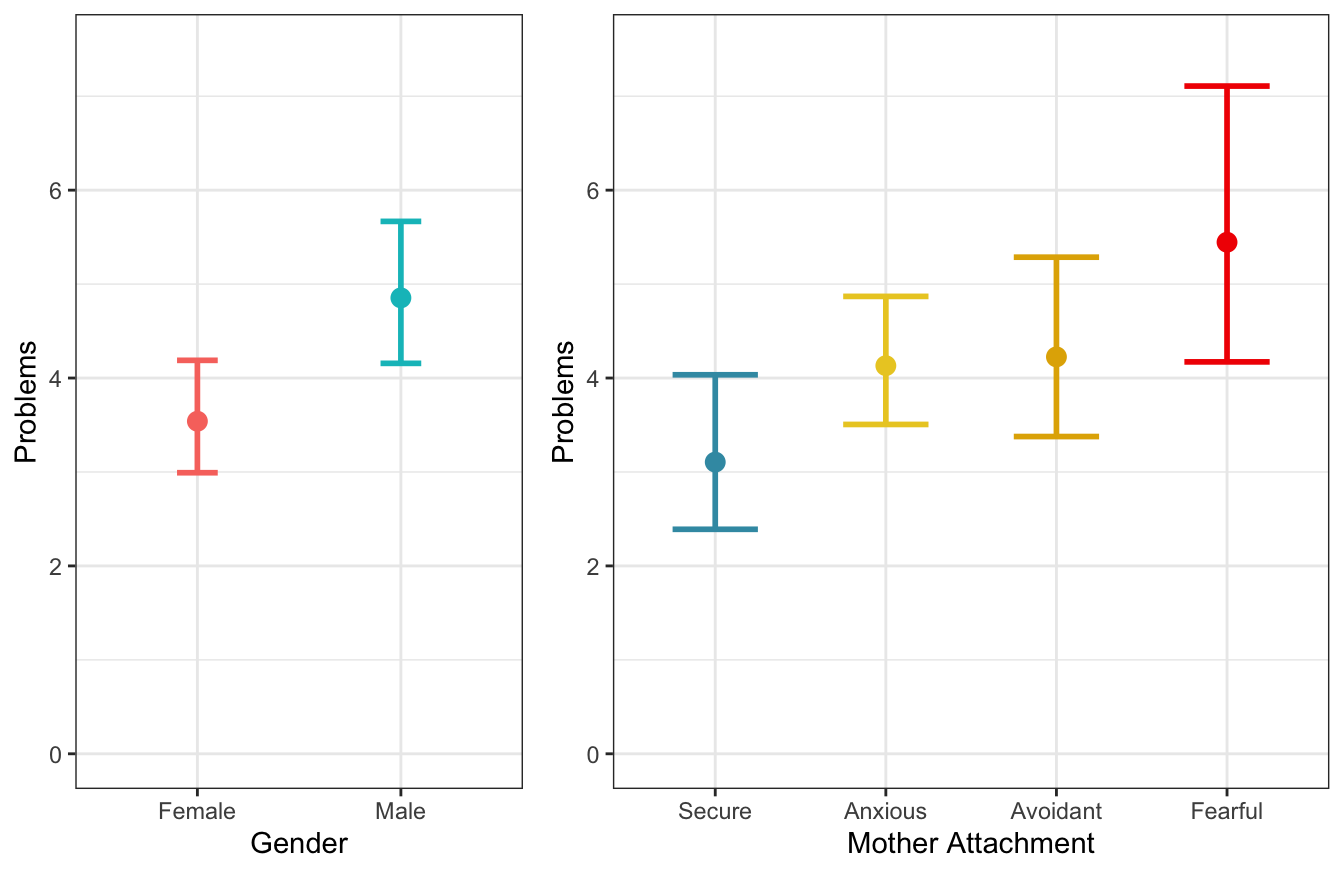
\includegraphics{attachment-bayes-factor_files/figure-latex/plot-nhst-effects-ext-1} 

}

\caption{Marginal predicted values according to gender and mother attachment. Values are averaged over the other effects ($n_{subj} = 847$).}\label{fig:plot-nhst-effects-ext}
\end{figure}

Post-hoc tests are run to evaluate differences between mother attachment styles. To do that we use the \texttt{contrast()} function from the \texttt{emmeans} R-package, considering pairwise comparisons and adjusting \emph{p}-values according to multivariate \emph{t}-distribution. This approach is less restrictive than the traditional \emph{``Bonferroni''} method, as it determines the adjustment according to a multivariate \emph{t}-distribution with the same covariance structure as the estimates. Results are reported below,

\begin{Shaded}
\begin{Highlighting}[]
\NormalTok{emmeans}\SpecialCharTok{::}\FunctionTok{contrast}\NormalTok{(emmeans}\SpecialCharTok{::}\FunctionTok{emmeans}\NormalTok{(fit\_ext\_zinb, }\AttributeTok{specs =} \SpecialCharTok{\textasciitilde{}}\NormalTok{ mother ),}
                  \StringTok{"pairwise"}\NormalTok{, }\AttributeTok{adjust =} \StringTok{"mvt"}\NormalTok{)}
\DocumentationTok{\#\# }\AlertTok{NOTE}\DocumentationTok{: Results may be misleading due to involvement in interactions}
\DocumentationTok{\#\#  contrast           estimate    SE  df t.ratio p.value}
\DocumentationTok{\#\#  Secure {-} Anxious    {-}0.2856 0.140 825  {-}2.034  0.1719}
\DocumentationTok{\#\#  Secure {-} Avoidant   {-}0.3080 0.162 825  {-}1.902  0.2228}
\DocumentationTok{\#\#  Secure {-} Fearful    {-}0.5617 0.178 825  {-}3.149  0.0089}
\DocumentationTok{\#\#  Anxious {-} Avoidant  {-}0.0224 0.124 825  {-}0.181  0.9978}
\DocumentationTok{\#\#  Anxious {-} Fearful   {-}0.2761 0.146 825  {-}1.885  0.2300}
\DocumentationTok{\#\#  Avoidant {-} Fearful  {-}0.2537 0.167 825  {-}1.522  0.4179}
\DocumentationTok{\#\# }
\DocumentationTok{\#\# Results are averaged over the levels of: gender, father }
\DocumentationTok{\#\# Results are given on the log (not the response) scale. }
\DocumentationTok{\#\# P value adjustment: mvt method for 6 tests}
\end{Highlighting}
\end{Shaded}

Overall, results indicate that Males have more externalizing problems than Females and, regarding mother attachment, Fearful children have more problems than Secure children.

To evaluate the fit of the model to the data, we used \(R^2\). In the case of generalized mixed-effects models, however, there are several definitions of \(R^2\). We computed the \emph{Marginal} \(R^2\) and the \emph{Conditional} \(R^2\) as suggested by \citet{nakagawaCoefficientDeterminationR22017}. \emph{Marginal} \(R^2\) is concerned with the variance explained by fixed factors of the model, and \emph{Conditional} \(R^2\) is concerned with the variance explained by both fixed and random factors of the model. To do that we use the function \texttt{performance::r2()}.

\begin{Shaded}
\begin{Highlighting}[]
\NormalTok{performance}\SpecialCharTok{::}\FunctionTok{r2}\NormalTok{(fit\_ext\_zinb)}
\DocumentationTok{\#\# Warning: mu of 4.2 is too close to zero, estimate of random effect variances may}
\DocumentationTok{\#\#   be unreliable.}
\DocumentationTok{\#\# \# R2 for Mixed Models}
\DocumentationTok{\#\# }
\DocumentationTok{\#\#   Conditional R2: 0.191}
\DocumentationTok{\#\#      Marginal R2: 0.091}
\end{Highlighting}
\end{Shaded}

We can see that the actual variance explained by fixed effects is almost 10\%, not bad for psychology.

\hypertarget{conclusions}{%
\subsubsection*{Conclusions}\label{conclusions}}
\addcontentsline{toc}{subsubsection}{Conclusions}

Considering attachment theoretical perspectives, results indicate only the role of mother attachment. Note, however, that traditional NHST does not allow us to evaluate evidence in favour of a hypothesis. Moreover, we actually have not tested our hypotheses but only the catch-all null hypothesis that \emph{``nothing is going on''}.

\hypertarget{model-comparison-ext}{%
\chapter{Model Comparison}\label{model-comparison-ext}}

Model comparison allows us to compare multiple hypotheses and identify which is the most supported by the data \citep{mcelreathStatisticalRethinkingBayesian2020}. First, we need to formalize models according to our hypotheses. Subsequently, we can evaluate which is the most supported model among those considered according to the data using the AIC and BIC \citep{wagenmakersAICModelSelection2004, akaike1973a, schwarzEstimatingDimensionModel1978}.

\hypertarget{formalize-models}{%
\section{Formalize Models}\label{formalize-models}}

Following the same reasons as before (see Section\textasciitilde\ref{model-choice-ext}), we consider Zero Inflated Negative Binomial Mixed-Effects models. Again, we consider only the role of gender as a fixed effect and children's classroom ID as a random effect for \(p\). Whereas, considering \(\mu\), we define four different models to take into account the different theoretical perspectives:

\begin{itemize}
\tightlist
\item
  \texttt{fit\_ext\_zero}: we consider only the effect of gender. This model assumes that attachment plays no role.
\item
  \texttt{fit\_ext\_mother}: we consider the additive effects of gender and mother attachment. This model supports the idea that only mother attachment is important (\textbf{Monotropy Theory}).
\item
  \texttt{fit\_ext\_additive}: we consider the additive effects of gender, mother attachment, and father attachment. This model supports the idea that both mother attachment and father attachment are important, but not their interaction (\textbf{Hierarchy Theory} or \textbf{Independence Theory}).
\item
  \texttt{fit\_ext\_inter}: we consider the additive effects of gender and the interaction between mother attachment and father attachment. This model supports the idea that the interaction between mother attachment and father attachment is important (\textbf{Integration Theory}).
\end{itemize}

Moreover, in all models, we include children's classroom ID as a random effect to take into account teachers' different ability to evaluate children's problems. Using R formula syntax, we have

\begin{Shaded}
\begin{Highlighting}[]
\CommentTok{\# formula for p (same for all models)}
\NormalTok{p }\SpecialCharTok{\textasciitilde{}}\NormalTok{ gender }\SpecialCharTok{+}\NormalTok{ (}\DecValTok{1}\SpecialCharTok{|}\NormalTok{ID\_class)}

\CommentTok{\# formula for mu}

\CommentTok{\# fit\_ext\_zero}
\NormalTok{mu }\SpecialCharTok{\textasciitilde{}}\NormalTok{ gender }\SpecialCharTok{+}\NormalTok{ (}\DecValTok{1}\SpecialCharTok{|}\NormalTok{ID\_class)}

\CommentTok{\# fit\_ext\_mother}
\NormalTok{mu }\SpecialCharTok{\textasciitilde{}}\NormalTok{ gender }\SpecialCharTok{+}\NormalTok{ mother }\SpecialCharTok{+}\NormalTok{ (}\DecValTok{1}\SpecialCharTok{|}\NormalTok{ID\_class)}

\CommentTok{\# fit\_ext\_additive}
\NormalTok{mu }\SpecialCharTok{\textasciitilde{}}\NormalTok{ gender }\SpecialCharTok{+}\NormalTok{ mother }\SpecialCharTok{+}\NormalTok{ father }\SpecialCharTok{+}\NormalTok{ (}\DecValTok{1}\SpecialCharTok{|}\NormalTok{ID\_class)}

\CommentTok{\# fit\_ext\_inter}
\NormalTok{mu }\SpecialCharTok{\textasciitilde{}}\NormalTok{ gender }\SpecialCharTok{+}\NormalTok{ mother }\SpecialCharTok{*}\NormalTok{ father }\SpecialCharTok{+}\NormalTok{ (}\DecValTok{1}\SpecialCharTok{|}\NormalTok{ID\_class)}
\end{Highlighting}
\end{Shaded}

\hypertarget{aic-and-bic-results}{%
\section{AIC and BIC Results}\label{aic-and-bic-results}}

After estimating the models, the AIC and BIC values together with their relative weights are computed. Results are reported in Table\textasciitilde\ref{tab:table-AIC-BIC-weights-ext}.

\begin{table}[!h]

\caption{\label{tab:table-AIC-BIC-weights-ext}Model comparison externalizing problems ($n_{subj} = 847$).}
\centering
\resizebox{\linewidth}{!}{
\begin{tabular}[t]{rccc>{\centering\arraybackslash}m{1cm}cc>{\centering\arraybackslash}m{1cm}}
\toprule
\textbf{Model} & \textbf{Df} & \textbf{AIC} & \textbf{AIC$_{weights}$} & \textbf{ } & \textbf{BIC} & \textbf{BIC$_{weights}$} & \textbf{ }\\
\midrule
fit-ext-zero & 6 & 3865.1 & 0.00 & 
\includegraphics[width=0.33in, height=0.33in]{images/ball_AIC_ext_zero.png} & 3898.3 & 0.78 & 
\includegraphics[width=0.33in, height=0.33in]{images/ball_BIC_ext_zero.png}\\
fit-ext-mother & 9 & 3853.4 & 0.92 & 
\includegraphics[width=0.33in, height=0.33in]{images/ball_AIC_ext_mother.png} & 3900.8 & 0.22 & 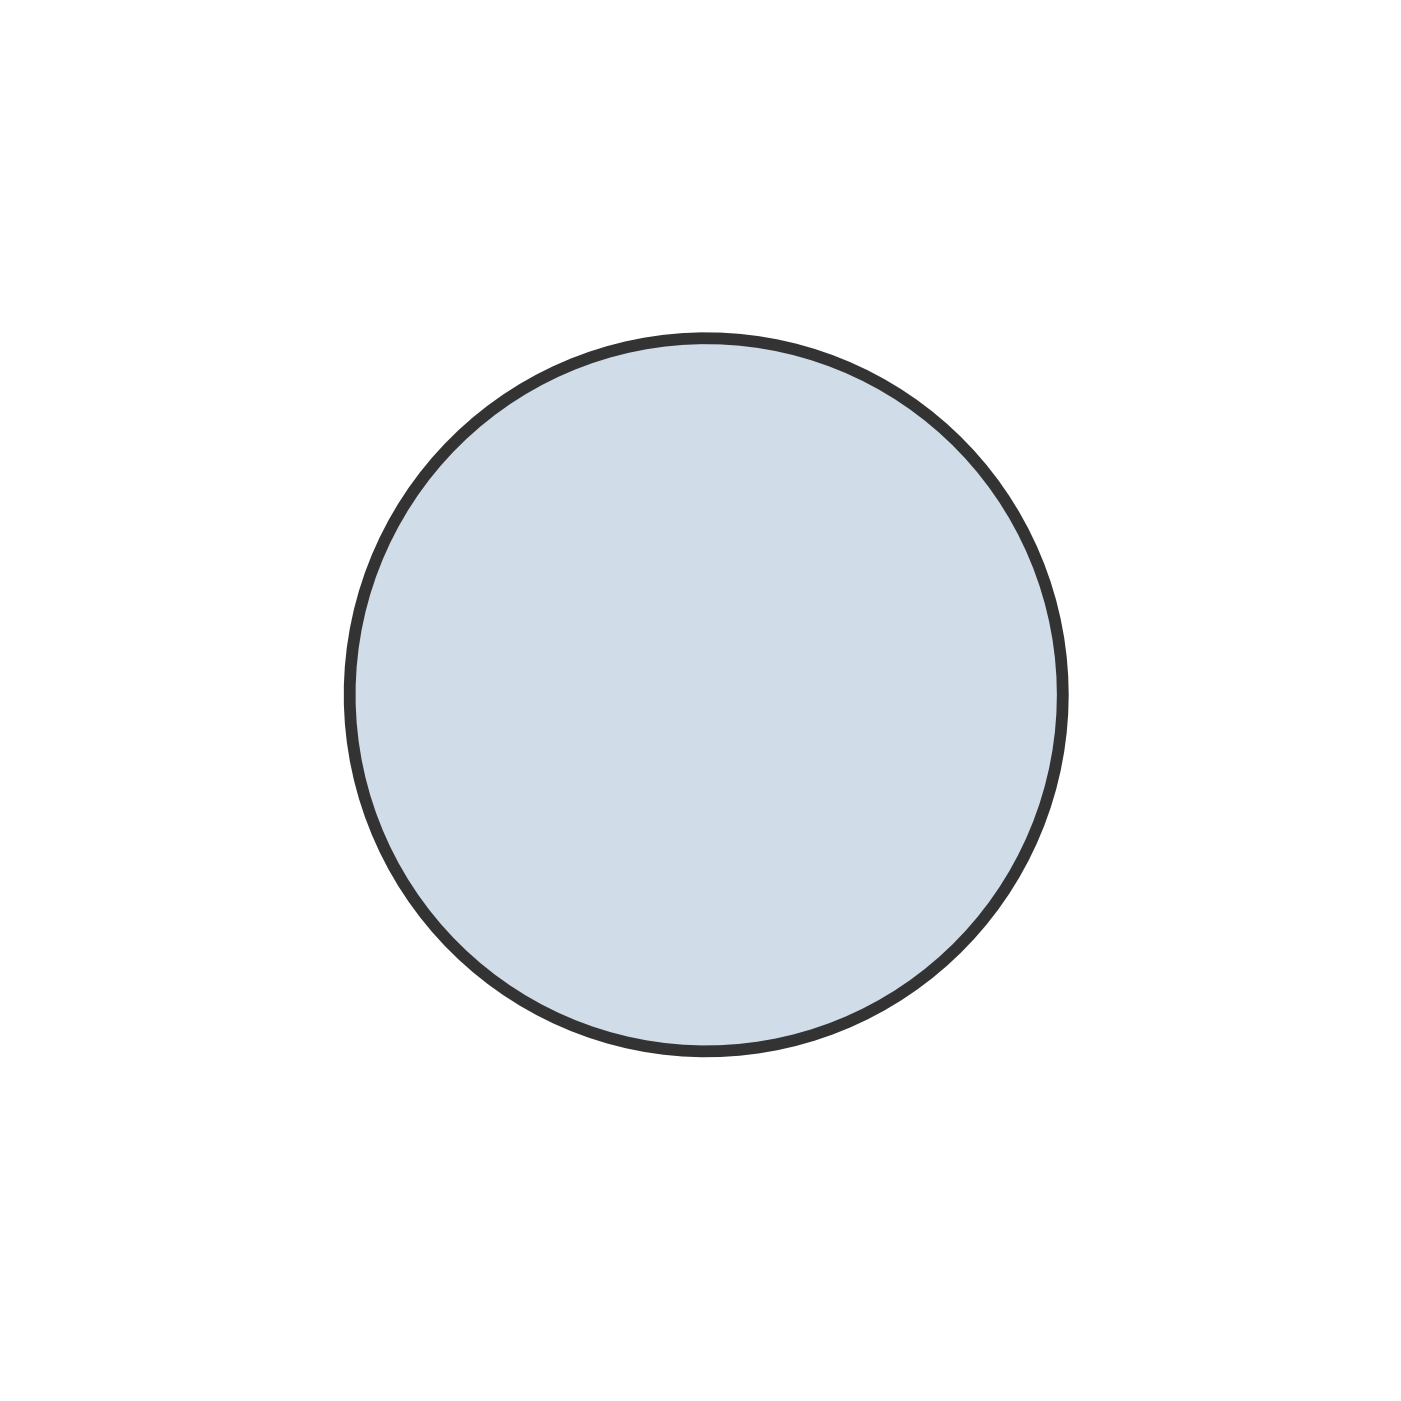
\includegraphics[width=0.33in, height=0.33in]{images/ball_BIC_ext_mother.png}\\
fit-ext-additive & 12 & 3858.4 & 0.08 & 
\includegraphics[width=0.33in, height=0.33in]{images/ball_AIC_ext_additive.png} & 3920.0 & 0.00 & 
\includegraphics[width=0.33in, height=0.33in]{images/ball_BIC_ext_additive.png}\\
fit-ext-inter & 21 & 3867.6 & 0.00 & 
\includegraphics[width=0.33in, height=0.33in]{images/ball_AIC_ext_inter.png} & 3971.9 & 0.00 & 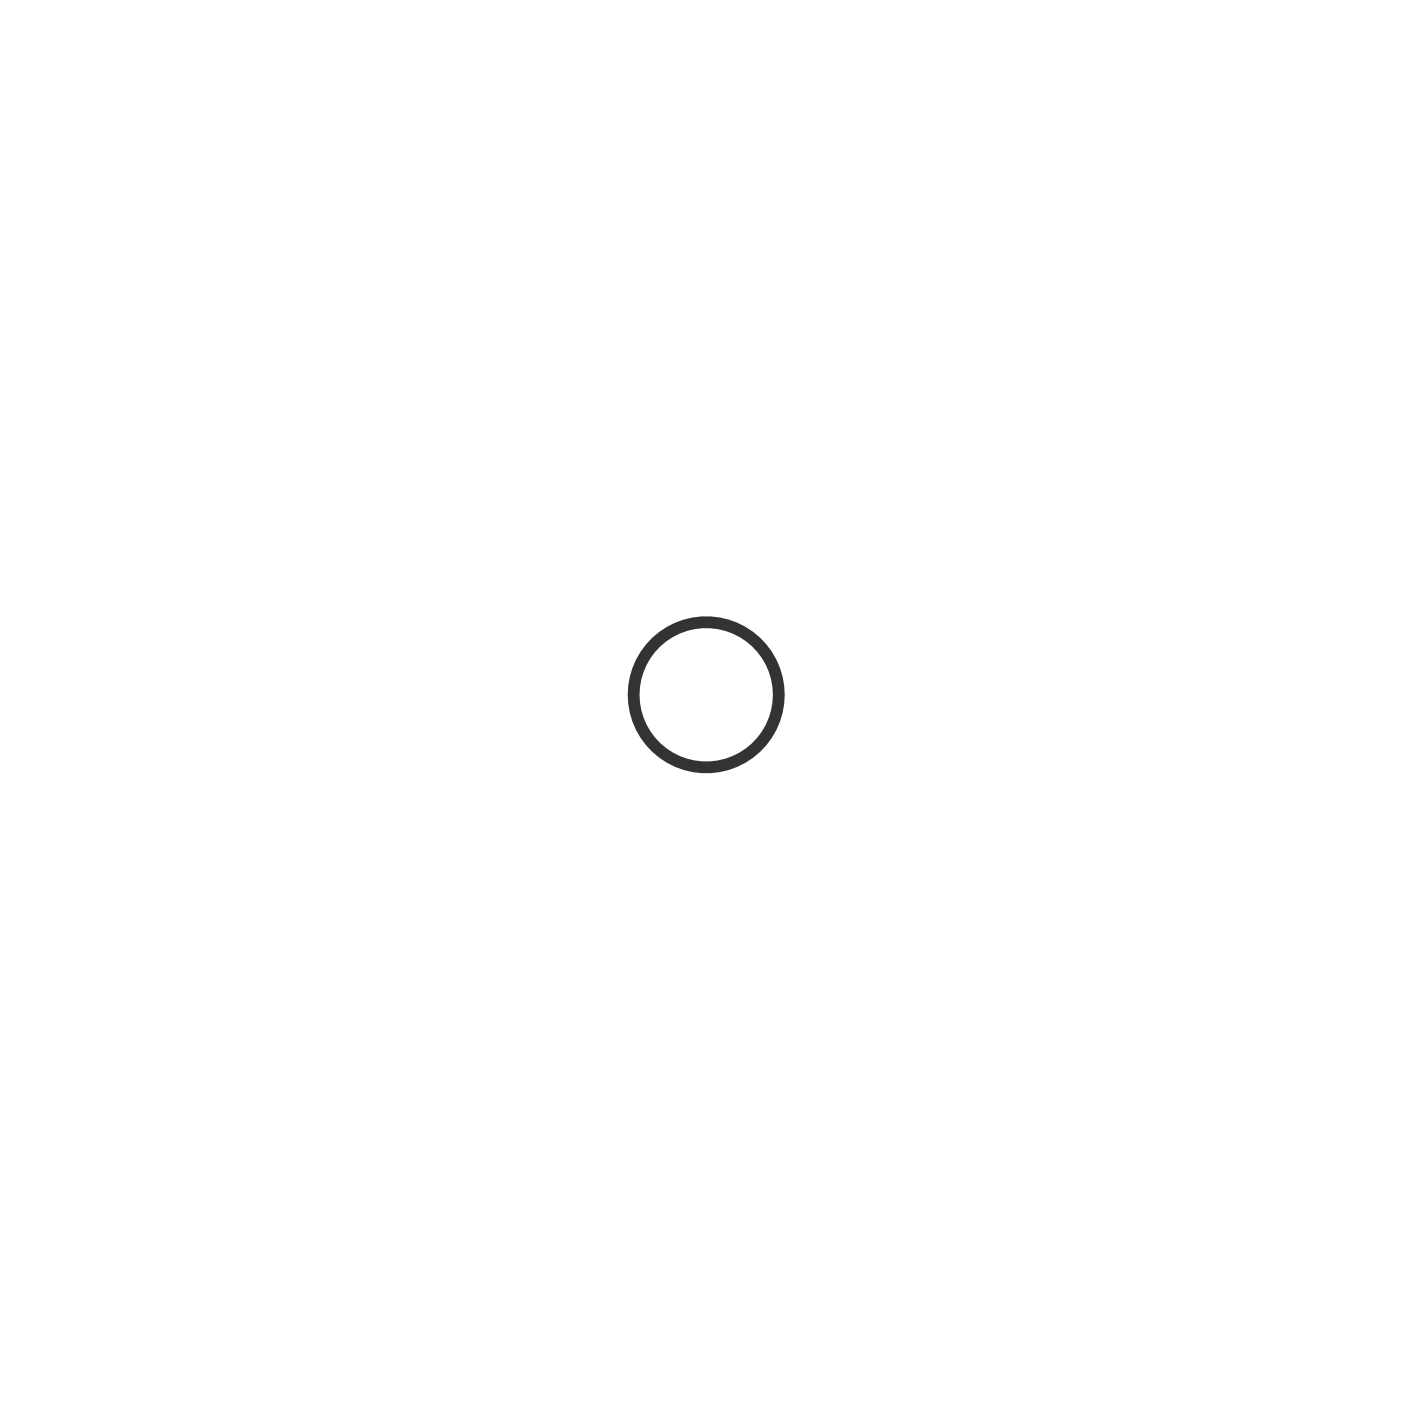
\includegraphics[width=0.33in, height=0.33in]{images/ball_BIC_ext_inter.png}\\
\bottomrule
\end{tabular}}
\end{table}

According to AIC, the most likely model is \texttt{fit\_ext\_mother} (92\%) and the second most likely model is \texttt{fit\_ext\_additive} (8\%) given the data and the set of models considered. According to BIC, instead, the most likely model is \texttt{fit\_ext\_zero} (78\%) and the second most likely model is \texttt{fit\_ext\_mother} (22\%) given the data and the set of models considered.

To interpret these results, note that, AIC tends to select more complex models that can better explain the data, on the contrary, BIC penalizes complex models to a greater extent. As pointed out by \citet{kuhaAICBICComparisons2004}, using the two criteria together is always advocated as agreement provides reassurance on the robustness of the results and disagreement still provides useful information for the discussion. We can say that there is evidence in favour of the role of mother attachment but probably this effect is small.

\hypertarget{selected-model}{%
\section{Selected Model}\label{selected-model}}

Considering the model \texttt{fit\_ext\_mother}, we can run an analysis of deviance to evaluate the significance of the predictors.

\begin{Shaded}
\begin{Highlighting}[]
\NormalTok{car}\SpecialCharTok{::}\FunctionTok{Anova}\NormalTok{(fit\_ext\_mother)}
\DocumentationTok{\#\# Analysis of Deviance Table (Type II Wald chisquare tests)}
\DocumentationTok{\#\# }
\DocumentationTok{\#\# Response: externalizing\_sum}
\DocumentationTok{\#\#         Chisq Df Pr(\textgreater{}Chisq)    }
\DocumentationTok{\#\# gender 17.732  1  2.544e{-}05 ***}
\DocumentationTok{\#\# mother 17.398  3  0.0005851 ***}
\DocumentationTok{\#\# {-}{-}{-}}
\DocumentationTok{\#\# Signif. codes:  0 \textquotesingle{}***\textquotesingle{} 0.001 \textquotesingle{}**\textquotesingle{} 0.01 \textquotesingle{}*\textquotesingle{} 0.05 \textquotesingle{}.\textquotesingle{} 0.1 \textquotesingle{} \textquotesingle{} 1}
\end{Highlighting}
\end{Shaded}

Results confirm a statistically significant effect of gender and mother attachment. The model summary is reported below.

\begin{Shaded}
\begin{Highlighting}[]
\FunctionTok{summary}\NormalTok{(fit\_ext\_mother)}
\DocumentationTok{\#\#  Family: nbinom2  ( log )}
\DocumentationTok{\#\# Formula:          externalizing\_sum \textasciitilde{} gender + mother + (1 | ID\_class)}
\DocumentationTok{\#\# Zero inflation:                     \textasciitilde{}gender + (1 | ID\_class)}
\DocumentationTok{\#\# Data: data\_cluster}
\DocumentationTok{\#\# }
\DocumentationTok{\#\#      AIC      BIC   logLik deviance df.resid }
\DocumentationTok{\#\#   3853.4   3900.8  {-}1916.7   3833.4      837 }
\DocumentationTok{\#\# }
\DocumentationTok{\#\# Random effects:}
\DocumentationTok{\#\# }
\DocumentationTok{\#\# Conditional model:}
\DocumentationTok{\#\#  Groups   Name        Variance Std.Dev.}
\DocumentationTok{\#\#  ID\_class (Intercept) 0.07747  0.2783  }
\DocumentationTok{\#\# Number of obs: 847, groups:  ID\_class, 50}
\DocumentationTok{\#\# }
\DocumentationTok{\#\# Zero{-}inflation model:}
\DocumentationTok{\#\#  Groups   Name        Variance Std.Dev.}
\DocumentationTok{\#\#  ID\_class (Intercept) 0.766    0.8752  }
\DocumentationTok{\#\# Number of obs: 847, groups:  ID\_class, 50}
\DocumentationTok{\#\# }
\DocumentationTok{\#\# Dispersion parameter for nbinom2 family (): 1.81 }
\DocumentationTok{\#\# }
\DocumentationTok{\#\# Conditional model:}
\DocumentationTok{\#\#                Estimate Std. Error z value Pr(\textgreater{}|z|)    }
\DocumentationTok{\#\# (Intercept)     0.98649    0.10770   9.160  \textless{} 2e{-}16 ***}
\DocumentationTok{\#\# genderM         0.33533    0.07964   4.211 2.54e{-}05 ***}
\DocumentationTok{\#\# motherAnxious   0.24321    0.10338   2.353  0.01864 *  }
\DocumentationTok{\#\# motherAvoidant  0.30803    0.10910   2.823  0.00475 ** }
\DocumentationTok{\#\# motherFearful   0.52680    0.13135   4.011 6.05e{-}05 ***}
\DocumentationTok{\#\# {-}{-}{-}}
\DocumentationTok{\#\# Signif. codes:  0 \textquotesingle{}***\textquotesingle{} 0.001 \textquotesingle{}**\textquotesingle{} 0.01 \textquotesingle{}*\textquotesingle{} 0.05 \textquotesingle{}.\textquotesingle{} 0.1 \textquotesingle{} \textquotesingle{} 1}
\DocumentationTok{\#\# }
\DocumentationTok{\#\# Zero{-}inflation model:}
\DocumentationTok{\#\#             Estimate Std. Error z value Pr(\textgreater{}|z|)    }
\DocumentationTok{\#\# (Intercept)  {-}1.1211     0.2432  {-}4.609 4.05e{-}06 ***}
\DocumentationTok{\#\# genderM      {-}0.6990     0.2491  {-}2.807    0.005 ** }
\DocumentationTok{\#\# {-}{-}{-}}
\DocumentationTok{\#\# Signif. codes:  0 \textquotesingle{}***\textquotesingle{} 0.001 \textquotesingle{}**\textquotesingle{} 0.01 \textquotesingle{}*\textquotesingle{} 0.05 \textquotesingle{}.\textquotesingle{} 0.1 \textquotesingle{} \textquotesingle{} 1}
\end{Highlighting}
\end{Shaded}

To evaluate the effect of gender and mother attachment, the marginal predicted values according to gender and mother attachment are presented separately in Figure\textasciitilde\ref{fig:plot-comparison-effects-ext}. Not that the marginal predicted values for gender are averaged over mother attachment. Whereas, the marginal predicted values for mother attachment are averaged over gender.

\begin{figure}

{\centering 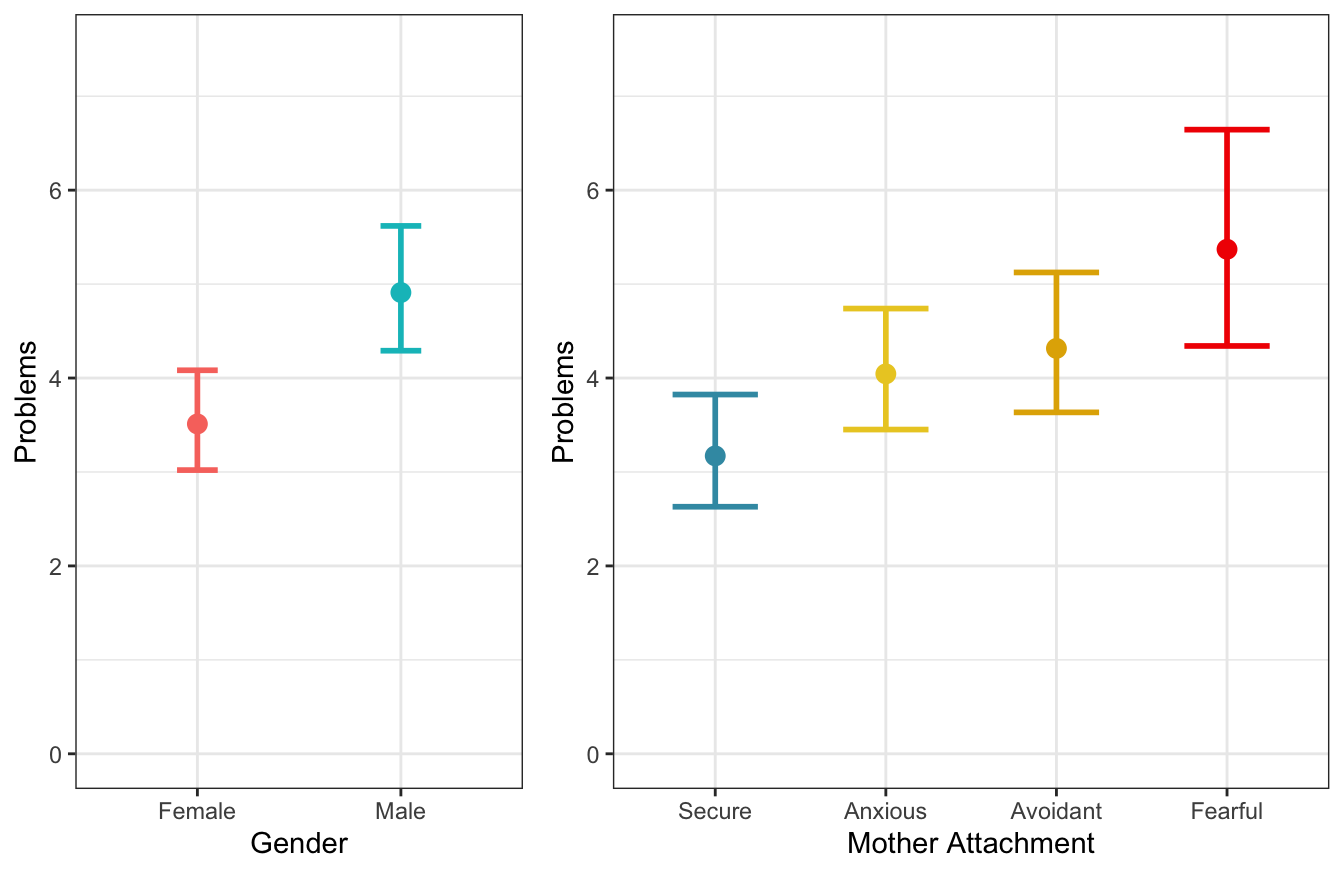
\includegraphics{attachment-bayes-factor_files/figure-latex/plot-comparison-effects-ext-1} 

}

\caption{Marginal predicted values according to gender and mother attachment ($n_{subj} = 847$).}\label{fig:plot-comparison-effects-ext}
\end{figure}

Post-hoc tests are run to evaluate differences between mother attachment styles, considering pairwise comparisons and adjusting \emph{p}-values according to multivariate \emph{t}-distribution. Results are reported below,

\begin{Shaded}
\begin{Highlighting}[]
\NormalTok{emmeans}\SpecialCharTok{::}\FunctionTok{contrast}\NormalTok{(emmeans}\SpecialCharTok{::}\FunctionTok{emmeans}\NormalTok{(fit\_ext\_mother, }\AttributeTok{specs =} \SpecialCharTok{\textasciitilde{}}\NormalTok{ mother ),}
                  \StringTok{"pairwise"}\NormalTok{, }\AttributeTok{adjust =} \StringTok{"mvt"}\NormalTok{)}
\DocumentationTok{\#\#  contrast           estimate     SE  df t.ratio p.value}
\DocumentationTok{\#\#  Secure {-} Anxious    {-}0.2432 0.1034 837  {-}2.353  0.0859}
\DocumentationTok{\#\#  Secure {-} Avoidant   {-}0.3080 0.1091 837  {-}2.823  0.0243}
\DocumentationTok{\#\#  Secure {-} Fearful    {-}0.5268 0.1313 837  {-}4.011  0.0004}
\DocumentationTok{\#\#  Anxious {-} Avoidant  {-}0.0648 0.0981 837  {-}0.661  0.9107}
\DocumentationTok{\#\#  Anxious {-} Fearful   {-}0.2836 0.1216 837  {-}2.333  0.0903}
\DocumentationTok{\#\#  Avoidant {-} Fearful  {-}0.2188 0.1276 837  {-}1.714  0.3135}
\DocumentationTok{\#\# }
\DocumentationTok{\#\# Results are averaged over the levels of: gender }
\DocumentationTok{\#\# Results are given on the log (not the response) scale. }
\DocumentationTok{\#\# P value adjustment: mvt method for 6 tests}
\end{Highlighting}
\end{Shaded}

Overall, results indicate that Males have more externalizing problems than Females. Regarding mother attachment, Fearful and Avoidant children have more problems than Secure children. Moreover, also the difference between Anxious and Secure children and the difference between Anxious and Fearful children have a low (but not statistically significant) \emph{p}-value.

To evaluate the fit of the model to the data, we computed the \emph{Marginal} \(R^2\) and the \emph{Conditional} \(R^2\).

\begin{Shaded}
\begin{Highlighting}[]
\NormalTok{performance}\SpecialCharTok{::}\FunctionTok{r2}\NormalTok{(fit\_ext\_mother)}
\DocumentationTok{\#\# Warning: mu of 4.2 is too close to zero, estimate of random effect variances may}
\DocumentationTok{\#\#   be unreliable.}
\DocumentationTok{\#\# \# R2 for Mixed Models}
\DocumentationTok{\#\# }
\DocumentationTok{\#\#   Conditional R2: 0.168}
\DocumentationTok{\#\#      Marginal R2: 0.071}
\end{Highlighting}
\end{Shaded}

We can see that the actual variance explained by fixed effects is around 7\%, not bad for psychology.

\hypertarget{conclusions-1}{%
\subsubsection*{Conclusions}\label{conclusions-1}}
\addcontentsline{toc}{subsubsection}{Conclusions}

Considering attachment theoretical perspectives, results indicate only the role of mother attachment so we can support the \textbf{Monotropy Theory}. Note, however, that the compared models contain no information regarding the expected direction of the effects but we only include/exclude predictors.

\hypertarget{BF-ext}{%
\chapter{Bayes Factor}\label{BF-ext}}

To properly evaluate hypotheses with information regarding the expected direction of the effects, we use the Bayes factor with the encompassing prior approach. See the main article for a detailed introduction to this approach {[}TODO: add link article{]}.

First, we define the encompassing model. Subsequently, we obtain the hypotheses matrices according to the informative hypotheses. Next, we compute the Bayes factor and, finally, we describe the selected model.

\hypertarget{encompassing-model}{%
\section{Encompassing Model}\label{encompassing-model}}

We define a Zero-Inflated Negative Binomial (ZINB) mixed-effects model to take into account the characteristics of the dependent variable and its distribution (see Section\textasciitilde\ref{model-choice-ext}). Again, we consider only the role of gender as a fixed effect and children's classroom ID as a random effect for \(p\). Whereas, regarding \(\mu\), we consider the interaction between mother and father attachment together with gender as fixed effects and children's classroom ID as a random effect. In the R formula syntax, we have

\begin{Shaded}
\begin{Highlighting}[]
\CommentTok{\# formula for p}
\NormalTok{p }\SpecialCharTok{\textasciitilde{}}\NormalTok{ gender }\SpecialCharTok{+}\NormalTok{ (}\DecValTok{1}\SpecialCharTok{|}\NormalTok{ID\_class)}

\CommentTok{\# formula for mu}
\NormalTok{mu }\SpecialCharTok{\textasciitilde{}}\NormalTok{ gender }\SpecialCharTok{+}\NormalTok{ mother }\SpecialCharTok{*}\NormalTok{ father }\SpecialCharTok{+}\NormalTok{ (}\DecValTok{1}\SpecialCharTok{|}\NormalTok{ID\_class)}
\end{Highlighting}
\end{Shaded}

\hypertarget{prior-choice}{%
\subsection{Prior Choice}\label{prior-choice}}

The prior choice is important for the parameters involved in the equality and inequality constraints. In our case, the parameters of interest (i.e., those related to mother and father attachment interaction) are unbounded. Thus, we can simply specify as prior a normal distribution with mean 0 and a given standard deviation. Considering the standard deviation, however, we have to choose a value so that the resulting prior is non-informative but without being excessively diffuse.

We can evaluate the consequences of different values' choice considering the resulting prior predictions. To facilitate this step, we compute prior prediction considering only the intercept and a single parameter of interest. Remembering that the inverse link function (i.e., function that in a GLM transform the model linear prediction into the value on the original response scale) is the exponential function, we consider as intercept the value 1 because \(exp(1) \approx 2.7\) that is close to the externalizing problems sample mean 3.35. In Table\textasciitilde\ref{tab:table-prior-predict}, summary information about prior predictions for different standard deviation values is reported.

\begin{table}[!h]

\caption{\label{tab:table-prior-predict}Prior prediction acording to different prior settings assuming $exp(1)$ as intercept value.}
\centering
\begin{tabular}[t]{rccccc}
\toprule
\multicolumn{1}{c}{ } & \multicolumn{5}{c}{Predicted Problems} \\
\cmidrule(l{3pt}r{3pt}){2-6}
Prior & $-1$ SD & $-.5$ SD & $+0$ SD & $+ .5$ SD & $+ 1$ SD\\
\midrule
$\mathcal{N}(0, 0.5)$ & 1.6 & 2.1 & 2.7 & 3.5 & 4.5\\
$\mathcal{N}(0, 1)$ & 1.0 & 1.6 & 2.7 & 4.5 & 7.4\\
$\mathcal{N}(0, 3)$ & 0.1 & 0.6 & 2.7 & 12.2 & 54.6\\
$\mathcal{N}(0, 5)$ & 0.0 & 0.2 & 2.7 & 33.1 & 403.4\\
$\mathcal{N}(0, 10)$ & 0.0 & 0.0 & 2.7 & 403.4 & 59874.1\\
\bottomrule
\end{tabular}
\end{table}

Considering that externalizing problems are bounded between 0 and 20, a reasonable prior is \(\mathcal{N}(0,3)\). With these settings, prior predicted values cover all possible values without including excessively large values. More diffuse priors would result in values with a higher order of magnitude and tighter priors would exclude plausible values. The influence of prior specification will be subsequently evaluated in a prior sensitivity analysis.

Regarding the other nuisance parameters (i.e., intercepts, random effects and shapes parameters) \texttt{brms} default priors are maintained. The resulting prior settings are

\begin{verbatim}
##                   prior     class                          coef    group resp dpar nlpar lb ub       source
##            normal(0, 3)         b                                                                      user
##            normal(0, 3)         b                 fatherAnxious                                (vectorized)
##            normal(0, 3)         b                fatherAvoidant                                (vectorized)
##            normal(0, 3)         b                 fatherFearful                                (vectorized)
##            normal(0, 3)         b                       genderM                                (vectorized)
##            normal(0, 3)         b                 motherAnxious                                (vectorized)
##            normal(0, 3)         b   motherAnxious:fatherAnxious                                (vectorized)
##            normal(0, 3)         b  motherAnxious:fatherAvoidant                                (vectorized)
##            normal(0, 3)         b   motherAnxious:fatherFearful                                (vectorized)
##            normal(0, 3)         b                motherAvoidant                                (vectorized)
##            normal(0, 3)         b  motherAvoidant:fatherAnxious                                (vectorized)
##            normal(0, 3)         b motherAvoidant:fatherAvoidant                                (vectorized)
##            normal(0, 3)         b  motherAvoidant:fatherFearful                                (vectorized)
##            normal(0, 3)         b                 motherFearful                                (vectorized)
##            normal(0, 3)         b   motherFearful:fatherAnxious                                (vectorized)
##            normal(0, 3)         b  motherFearful:fatherAvoidant                                (vectorized)
##            normal(0, 3)         b   motherFearful:fatherFearful                                (vectorized)
##                  (flat)         b                                               zi                  default
##                  (flat)         b                       genderM                 zi             (vectorized)
##  student_t(3, 0.7, 2.5) Intercept                                                                   default
##          logistic(0, 1) Intercept                                               zi                  default
##    student_t(3, 0, 2.5)        sd                                                         0         default
##    student_t(3, 0, 2.5)        sd                                               zi        0         default
##    student_t(3, 0, 2.5)        sd                               ID_class                  0    (vectorized)
##    student_t(3, 0, 2.5)        sd                     Intercept ID_class                  0    (vectorized)
##    student_t(3, 0, 2.5)        sd                               ID_class        zi        0    (vectorized)
##    student_t(3, 0, 2.5)        sd                     Intercept ID_class        zi        0    (vectorized)
##       gamma(0.01, 0.01)     shape                                                         0         default
\end{verbatim}

\hypertarget{posterior}{%
\subsection{Posterior}\label{posterior}}

The encompassing model is estimated using 6 independent chains with 10,000 iterations (warm-up 2,000). To do that we use the \texttt{brm()} function from the \texttt{brms} R-package \citep{burknerBrmsPackageBayesian2017, burknerAdvancedBayesianMultilevel2018a}, which is based on STAN \citep{standevelopmentteamRStanInterfaceStan2020}. Summary of the encompassing model is presented below.

\begin{verbatim}
##  Family: zero_inflated_negbinomial 
##   Links: mu = log; shape = identity; zi = logit 
## Formula: externalizing_sum ~ gender + mother * father + (1 | ID_class) 
##          zi ~ gender + (1 | ID_class)
##    Data: data (Number of observations: 847) 
##   Draws: 6 chains, each with iter = 10000; warmup = 2000; thin = 1;
##          total post-warmup draws = 48000
## 
## Group-Level Effects: 
## ~ID_class (Number of levels: 50) 
##                  Estimate Est.Error l-95% CI u-95% CI Rhat Bulk_ESS Tail_ESS
## sd(Intercept)        0.30      0.07     0.17     0.45 1.00    14452    20584
## sd(zi_Intercept)     1.14      0.29     0.68     1.82 1.00    21599    30432
## 
## Population-Level Effects: 
##                               Estimate Est.Error l-95% CI u-95% CI Rhat Bulk_ESS Tail_ESS
## Intercept                         0.98      0.13     0.72     1.24 1.00    36946    39083
## zi_Intercept                     -1.33      0.33    -2.08    -0.79 1.00    37409    31478
## genderM                           0.32      0.08     0.16     0.49 1.00    83483    38460
## motherAnxious                     0.32      0.19    -0.06     0.69 1.00    40607    39458
## motherAvoidant                    0.17      0.26    -0.33     0.69 1.00    39406    36276
## motherFearful                     0.69      0.41    -0.07     1.53 1.00    35752    33258
## fatherAnxious                     0.22      0.19    -0.16     0.60 1.00    41153    37645
## fatherAvoidant                   -0.45      0.21    -0.87    -0.03 1.00    43962    38015
## fatherFearful                     0.11      0.42    -0.68     0.97 1.00    33620    33965
## motherAnxious:fatherAnxious      -0.39      0.28    -0.93     0.15 1.00    37290    38104
## motherAvoidant:fatherAnxious     -0.12      0.34    -0.79     0.53 1.00    37877    36168
## motherFearful:fatherAnxious      -0.43      0.51    -1.45     0.55 1.00    36742    34591
## motherAnxious:fatherAvoidant      0.33      0.29    -0.24     0.89 1.00    38934    38185
## motherAvoidant:fatherAvoidant     0.60      0.33    -0.05     1.25 1.00    37462    34839
## motherFearful:fatherAvoidant      0.30      0.48    -0.67     1.20 1.00    34490    33126
## motherAnxious:fatherFearful      -0.06      0.48    -1.03     0.87 1.00    33089    34838
## motherAvoidant:fatherFearful      0.09      0.57    -1.04     1.19 1.00    35141    36840
## motherFearful:fatherFearful      -0.27      0.59    -1.46     0.86 1.00    29919    31952
## zi_genderM                       -0.78      0.29    -1.38    -0.24 1.00    68477    37227
## 
## Family Specific Parameters: 
##       Estimate Est.Error l-95% CI u-95% CI Rhat Bulk_ESS Tail_ESS
## shape     1.64      0.24     1.22     2.14 1.00    34980    35143
## 
## Draws were sampled using sampling(NUTS). For each parameter, Bulk_ESS
## and Tail_ESS are effective sample size measures, and Rhat is the potential
## scale reduction factor on split chains (at convergence, Rhat = 1).
\end{verbatim}

\hypertarget{hypothesis-matrices}{%
\section{Hypothesis Matrices}\label{hypothesis-matrices}}

For each informative hypothesis, we obtain a hypothesis matrix that translates equality and inequality constraints according to the encompassing model parametrization. Formalization of informative hypotheses and the procedure to derive hypothesis matrices are described in the main paper ({[}TODO: add link{]}).

Here we present the obtained hypothesis matrices where on the columns we have the parameters of the encompassing model (excluding the intercept) and each row expresses an equality constraint or an inequality constraint. Matrices' row names follow this notation: names without square brackets indicate a constraint directly on the model parameter; names within square brackets indicate a group condition (that could be the resulting composition of more parameters). For example, \texttt{"M\_Avoidant:F\_Anxious"} indicates the actual interaction term of the model, whereas \texttt{"{[}M\_Avoidant\_F\_Anxious{]}"} indicates the group condition. This is done because when assuming no interaction or no father attachment effect we set constraints directly on the model parameters, instead, when constraints involve group comparisons, we need to obtain the resulting conditions. Equality and inequality constraints are presented separately.

\hypertarget{null-hypothesis}{%
\subsubsection*{Null Hypothesis}\label{null-hypothesis}}
\addcontentsline{toc}{subsubsection}{Null Hypothesis}

\begin{itemize}
\tightlist
\item
  \textbf{Equality matrix}, \(R_{iE} = 0\) (each row is set to zero).
\end{itemize}

\begin{verbatim}
##                       M_Anxious M_Avoidant M_Fearful F_Anxious F_Avoidant F_Fearful M_Anxious:F_Anxious M_Avoidant:F_Anxious M_Fearful:F_Anxious M_Anxious:F_Avoidant M_Avoidant:F_Avoidant M_Fearful:F_Avoidant M_Anxious:F_Fearful M_Avoidant:F_Fearful M_Fearful:F_Fearful
## M_Anxious                     1          0         0         0          0         0                   0                    0                   0                    0                     0                    0                   0                    0                   0
## M_Avoidant                    0          1         0         0          0         0                   0                    0                   0                    0                     0                    0                   0                    0                   0
## M_Fearful                     0          0         1         0          0         0                   0                    0                   0                    0                     0                    0                   0                    0                   0
## F_Anxious                     0          0         0         1          0         0                   0                    0                   0                    0                     0                    0                   0                    0                   0
## F_Avoidant                    0          0         0         0          1         0                   0                    0                   0                    0                     0                    0                   0                    0                   0
## F_Fearful                     0          0         0         0          0         1                   0                    0                   0                    0                     0                    0                   0                    0                   0
## M_Anxious:F_Anxious           0          0         0         0          0         0                   1                    0                   0                    0                     0                    0                   0                    0                   0
## M_Avoidant:F_Anxious          0          0         0         0          0         0                   0                    1                   0                    0                     0                    0                   0                    0                   0
## M_Fearful:F_Anxious           0          0         0         0          0         0                   0                    0                   1                    0                     0                    0                   0                    0                   0
## M_Anxious:F_Avoidant          0          0         0         0          0         0                   0                    0                   0                    1                     0                    0                   0                    0                   0
## M_Avoidant:F_Avoidant         0          0         0         0          0         0                   0                    0                   0                    0                     1                    0                   0                    0                   0
## M_Fearful:F_Avoidant          0          0         0         0          0         0                   0                    0                   0                    0                     0                    1                   0                    0                   0
## M_Anxious:F_Fearful           0          0         0         0          0         0                   0                    0                   0                    0                     0                    0                   1                    0                   0
## M_Avoidant:F_Fearful          0          0         0         0          0         0                   0                    0                   0                    0                     0                    0                   0                    1                   0
## M_Fearful:F_Fearful           0          0         0         0          0         0                   0                    0                   0                    0                     0                    0                   0                    0                   1
\end{verbatim}

\begin{itemize}
\tightlist
\item
  \textbf{Inequality matrix}, \(R_{iI} > 0\) (each row is set greater than zero). There are no inequality constraints.
\end{itemize}

\hypertarget{monotropy-hypothesis}{%
\subsubsection*{Monotropy Hypothesis}\label{monotropy-hypothesis}}
\addcontentsline{toc}{subsubsection}{Monotropy Hypothesis}

\begin{itemize}
\tightlist
\item
  \textbf{Equality matrix}, \(R_{iE} = 0\) (each row is set to zero).
\end{itemize}

\begin{verbatim}
##                            M_Anxious M_Avoidant M_Fearful F_Anxious F_Avoidant F_Fearful M_Anxious:F_Anxious M_Avoidant:F_Anxious M_Fearful:F_Anxious M_Anxious:F_Avoidant M_Avoidant:F_Avoidant M_Fearful:F_Avoidant M_Anxious:F_Fearful M_Avoidant:F_Fearful M_Fearful:F_Fearful
## [M_Anx_F_Sec - M_Av_F_Sec]         1         -1         0         0          0         0                   0                    0                   0                    0                     0                    0                   0                    0                   0
## F_Anxious                          0          0         0         1          0         0                   0                    0                   0                    0                     0                    0                   0                    0                   0
## F_Avoidant                         0          0         0         0          1         0                   0                    0                   0                    0                     0                    0                   0                    0                   0
## F_Fearful                          0          0         0         0          0         1                   0                    0                   0                    0                     0                    0                   0                    0                   0
## M_Anxious:F_Anxious                0          0         0         0          0         0                   1                    0                   0                    0                     0                    0                   0                    0                   0
## M_Avoidant:F_Anxious               0          0         0         0          0         0                   0                    1                   0                    0                     0                    0                   0                    0                   0
## M_Fearful:F_Anxious                0          0         0         0          0         0                   0                    0                   1                    0                     0                    0                   0                    0                   0
## M_Anxious:F_Avoidant               0          0         0         0          0         0                   0                    0                   0                    1                     0                    0                   0                    0                   0
## M_Avoidant:F_Avoidant              0          0         0         0          0         0                   0                    0                   0                    0                     1                    0                   0                    0                   0
## M_Fearful:F_Avoidant               0          0         0         0          0         0                   0                    0                   0                    0                     0                    1                   0                    0                   0
## M_Anxious:F_Fearful                0          0         0         0          0         0                   0                    0                   0                    0                     0                    0                   1                    0                   0
## M_Avoidant:F_Fearful               0          0         0         0          0         0                   0                    0                   0                    0                     0                    0                   0                    1                   0
## M_Fearful:F_Fearful                0          0         0         0          0         0                   0                    0                   0                    0                     0                    0                   0                    0                   1
\end{verbatim}

\begin{itemize}
\tightlist
\item
  \textbf{Inequality matrix}, \(R_{iI} > 0\) (each row is set greater than zero).
\end{itemize}

\begin{verbatim}
##                             M_Anxious M_Avoidant M_Fearful F_Anxious F_Avoidant F_Fearful M_Anxious:F_Anxious M_Avoidant:F_Anxious M_Fearful:F_Anxious M_Anxious:F_Avoidant M_Avoidant:F_Avoidant M_Fearful:F_Avoidant M_Anxious:F_Fearful M_Avoidant:F_Fearful M_Fearful:F_Fearful
## [M_Anx_F_Sec]                       1          0         0         0          0         0                   0                    0                   0                    0                     0                    0                   0                    0                   0
## [M_Fear_F_Sec - M_Av_F_Sec]         0         -1         1         0          0         0                   0                    0                   0                    0                     0                    0                   0                    0                   0
\end{verbatim}

\hypertarget{hierarchy-hypothesis}{%
\subsubsection*{Hierarchy Hypothesis}\label{hierarchy-hypothesis}}
\addcontentsline{toc}{subsubsection}{Hierarchy Hypothesis}

\begin{itemize}
\tightlist
\item
  \textbf{Equality matrix}, \(R_{iE} = 0\) (each row is set to zero).
\end{itemize}

\begin{verbatim}
##                            M_Anxious M_Avoidant M_Fearful F_Anxious F_Avoidant F_Fearful M_Anxious:F_Anxious M_Avoidant:F_Anxious M_Fearful:F_Anxious M_Anxious:F_Avoidant M_Avoidant:F_Avoidant M_Fearful:F_Avoidant M_Anxious:F_Fearful M_Avoidant:F_Fearful M_Fearful:F_Fearful
## [M_Anx_F_Sec - M_Av_F_Sec]         1         -1         0         0          0         0                   0                    0                   0                    0                     0                    0                   0                    0                   0
## [M_Sec_F_Anx - M_Sec_F_Av]         0          0         0         1         -1         0                   0                    0                   0                    0                     0                    0                   0                    0                   0
## M_Anxious:F_Anxious                0          0         0         0          0         0                   1                    0                   0                    0                     0                    0                   0                    0                   0
## M_Avoidant:F_Anxious               0          0         0         0          0         0                   0                    1                   0                    0                     0                    0                   0                    0                   0
## M_Fearful:F_Anxious                0          0         0         0          0         0                   0                    0                   1                    0                     0                    0                   0                    0                   0
## M_Anxious:F_Avoidant               0          0         0         0          0         0                   0                    0                   0                    1                     0                    0                   0                    0                   0
## M_Avoidant:F_Avoidant              0          0         0         0          0         0                   0                    0                   0                    0                     1                    0                   0                    0                   0
## M_Fearful:F_Avoidant               0          0         0         0          0         0                   0                    0                   0                    0                     0                    1                   0                    0                   0
## M_Anxious:F_Fearful                0          0         0         0          0         0                   0                    0                   0                    0                     0                    0                   1                    0                   0
## M_Avoidant:F_Fearful               0          0         0         0          0         0                   0                    0                   0                    0                     0                    0                   0                    1                   0
## M_Fearful:F_Fearful                0          0         0         0          0         0                   0                    0                   0                    0                     0                    0                   0                    0                   1
\end{verbatim}

\begin{itemize}
\tightlist
\item
  \textbf{Inequality matrix}, \(R_{iI} > 0\) (each row is set greater than zero).
\end{itemize}

\begin{verbatim}
##                               M_Anxious M_Avoidant M_Fearful F_Anxious F_Avoidant F_Fearful M_Anxious:F_Anxious M_Avoidant:F_Anxious M_Fearful:F_Anxious M_Anxious:F_Avoidant M_Avoidant:F_Avoidant M_Fearful:F_Avoidant M_Anxious:F_Fearful M_Avoidant:F_Fearful M_Fearful:F_Fearful
## [M_Anx_F_Sec]                         1          0         0         0          0         0                   0                    0                   0                    0                     0                    0                   0                    0                   0
## [M_Fear_F_Sec - M_Av_F_Sec]           0         -1         1         0          0         0                   0                    0                   0                    0                     0                    0                   0                    0                   0
## [M_Sec_F_Anx]                         0          0         0         1          0         0                   0                    0                   0                    0                     0                    0                   0                    0                   0
## [M_Sec_F_Fear - M_Sec_F_Av]           0          0         0         0         -1         1                   0                    0                   0                    0                     0                    0                   0                    0                   0
## [M_Anx_F_Sec - M_Sec_F_Anx]           1          0         0        -1          0         0                   0                    0                   0                    0                     0                    0                   0                    0                   0
## [M_Av_F_Sec - M_Sec_F_Av]             0          1         0         0         -1         0                   0                    0                   0                    0                     0                    0                   0                    0                   0
## [M_Fear_F_Sec - M_Sec_F_Fear]         0          0         1         0          0        -1                   0                    0                   0                    0                     0                    0                   0                    0                   0
\end{verbatim}

\hypertarget{independence-hypothesis}{%
\subsubsection*{Independence Hypothesis}\label{independence-hypothesis}}
\addcontentsline{toc}{subsubsection}{Independence Hypothesis}

\begin{itemize}
\tightlist
\item
  \textbf{Equality matrix}, \(R_{iE} = 0\) (each row is set to zero).
\end{itemize}

\begin{verbatim}
##                            M_Anxious M_Avoidant M_Fearful F_Anxious F_Avoidant F_Fearful M_Anxious:F_Anxious M_Avoidant:F_Anxious M_Fearful:F_Anxious M_Anxious:F_Avoidant M_Avoidant:F_Avoidant M_Fearful:F_Avoidant M_Anxious:F_Fearful M_Avoidant:F_Fearful M_Fearful:F_Fearful
## [M_Anx_F_Sec - M_Av_F_Sec]         1         -1         0         0          0         0                   0                    0                   0                    0                     0                    0                   0                    0                   0
## M_Anxious:F_Anxious                0          0         0         0          0         0                   1                    0                   0                    0                     0                    0                   0                    0                   0
## M_Avoidant:F_Anxious               0          0         0         0          0         0                   0                    1                   0                    0                     0                    0                   0                    0                   0
## M_Fearful:F_Anxious                0          0         0         0          0         0                   0                    0                   1                    0                     0                    0                   0                    0                   0
## M_Anxious:F_Avoidant               0          0         0         0          0         0                   0                    0                   0                    1                     0                    0                   0                    0                   0
## M_Avoidant:F_Avoidant              0          0         0         0          0         0                   0                    0                   0                    0                     1                    0                   0                    0                   0
## M_Fearful:F_Avoidant               0          0         0         0          0         0                   0                    0                   0                    0                     0                    1                   0                    0                   0
## M_Anxious:F_Fearful                0          0         0         0          0         0                   0                    0                   0                    0                     0                    0                   1                    0                   0
## M_Avoidant:F_Fearful               0          0         0         0          0         0                   0                    0                   0                    0                     0                    0                   0                    1                   0
## M_Fearful:F_Fearful                0          0         0         0          0         0                   0                    0                   0                    0                     0                    0                   0                    0                   1
\end{verbatim}

\begin{itemize}
\tightlist
\item
  \textbf{Inequality matrix}, \(R_{iI} > 0\) (each row is set greater than zero).
\end{itemize}

\begin{verbatim}
##                             M_Anxious M_Avoidant M_Fearful F_Anxious F_Avoidant F_Fearful M_Anxious:F_Anxious M_Avoidant:F_Anxious M_Fearful:F_Anxious M_Anxious:F_Avoidant M_Avoidant:F_Avoidant M_Fearful:F_Avoidant M_Anxious:F_Fearful M_Avoidant:F_Fearful M_Fearful:F_Fearful
## [M_Anx_F_Sec]                       1          0         0         0          0         0                   0                    0                   0                    0                     0                    0                   0                    0                   0
## [M_Fear_F_Sec - M_Av_F_Sec]         0         -1         1         0          0         0                   0                    0                   0                    0                     0                    0                   0                    0                   0
## [M_Sec_F_Anx]                       0          0         0         1          0         0                   0                    0                   0                    0                     0                    0                   0                    0                   0
## [M_Sec_F_Av - M_Sec_F_Anx]          0          0         0        -1          1         0                   0                    0                   0                    0                     0                    0                   0                    0                   0
## [M_Sec_F_Fear - M_Sec_F_Av]         0          0         0         0         -1         1                   0                    0                   0                    0                     0                    0                   0                    0                   0
\end{verbatim}

\hypertarget{integration-hypothesis}{%
\subsubsection*{Integration Hypothesis}\label{integration-hypothesis}}
\addcontentsline{toc}{subsubsection}{Integration Hypothesis}

\begin{itemize}
\tightlist
\item
  \textbf{Equality matrix}, \(R_{iE} = 0\) (each row is set to zero).
\end{itemize}

\begin{verbatim}
##                               M_Anxious M_Avoidant M_Fearful F_Anxious F_Avoidant F_Fearful M_Anxious:F_Anxious M_Avoidant:F_Anxious M_Fearful:F_Anxious M_Anxious:F_Avoidant M_Avoidant:F_Avoidant M_Fearful:F_Avoidant M_Anxious:F_Fearful M_Avoidant:F_Fearful M_Fearful:F_Fearful
## [M_Anx_F_Sec - M_Av_F_Sec]            1         -1         0         0          0         0                   0                    0                   0                    0                     0                    0                   0                    0                   0
## [M_Anx_F_Sec - M_Sec_F_Anx]           1          0         0        -1          0         0                   0                    0                   0                    0                     0                    0                   0                    0                   0
## [M_Anx_F_Sec - M_Sec_F_Av]            1          0         0         0         -1         0                   0                    0                   0                    0                     0                    0                   0                    0                   0
## [M_Anx_F_Anx - M_Anx_F_Av]            0          0         0         1         -1         0                   1                    0                   0                   -1                     0                    0                   0                    0                   0
## [M_Anx_F_Anx - M_Av_F_Anx]            1         -1         0         0          0         0                   1                   -1                   0                    0                     0                    0                   0                    0                   0
## [M_Anx_F_Anx - M_Av_F_Av]             1         -1         0         1         -1         0                   1                    0                   0                    0                    -1                    0                   0                    0                   0
## [M_Fear_F_Anx - M_Fear_F_Av]          0          0         0         1         -1         0                   0                    0                   1                    0                     0                   -1                   0                    0                   0
## [M_Fear_F_Anx - M_Anx_F_Fear]        -1          0         1         1          0        -1                   0                    0                   1                    0                     0                    0                  -1                    0                   0
## [M_Fear_F_Anx - M_Av_F_Fear]          0         -1         1         1          0        -1                   0                    0                   1                    0                     0                    0                   0                   -1                   0
\end{verbatim}

\begin{itemize}
\tightlist
\item
  \textbf{Inequality matrix}, \(R_{iI} > 0\) (each row is set greater than zero).
\end{itemize}

\begin{verbatim}
##                                M_Anxious M_Avoidant M_Fearful F_Anxious F_Avoidant F_Fearful M_Anxious:F_Anxious M_Avoidant:F_Anxious M_Fearful:F_Anxious M_Anxious:F_Avoidant M_Avoidant:F_Avoidant M_Fearful:F_Avoidant M_Anxious:F_Fearful M_Avoidant:F_Fearful M_Fearful:F_Fearful
## [M_Anx_F_Sec]                          1          0         0         0          0         0                   0                    0                   0                    0                     0                    0                   0                    0                   0
## [M_Anx_F_Anx - M_Anx_F_Sec]            0          0         0         1          0         0                   1                    0                   0                    0                     0                    0                   0                    0                   0
## [M_Fear_F_Anx - M_Anx_F_Anx]          -1          0         1         0          0         0                  -1                    0                   1                    0                     0                    0                   0                    0                   0
## [M_Fear_F_Fear - M_Fear_F_Anx]         0          0         0        -1          0         1                   0                    0                  -1                    0                     0                    0                   0                    0                   1
\end{verbatim}

\hypertarget{centering-and-adjusting}{%
\section{Centering and Adjusting}\label{centering-and-adjusting}}

So far we have specified the encompassing prior, obtained the model posterior distribution, and defined the hypotheses matrices. Now, we need to transform our parameters of interest and center the distribution on the constraints focal points of interest. We apply the following transformation
\[
\beta = R\theta - r
\]
but we can ignore \(r\) as in all our constraints it is always a vector of zeros.

Next, we get the adjusted prior and the posterior of the transformed parameters vector \(\beta\) (i.e., the parameters that identify the constraints) for each hypothesis. The adjusted prior is given by

\[
\pi_{adj}(\beta) \sim \mathcal{N}(0, \Sigma_{\beta}) = \mathcal{N}(0, R\Sigma_{\theta}R^T).
\]
Note that we set the mean vector to zero. The posterior is given by the same transformation
\[
Pr(\beta|Y) \sim \mathcal{N}(\hat{\beta}, \hat{\Sigma}_{\beta}) = \mathcal{N}(R\hat{\theta}-r, R\hat{\Sigma}_{\theta}R^T).
\]
See the main article for more details {[}TODO: add link{]}.

This adjustment, however, requires the hypothesis matrix \(R\) to be \emph{full-row-rank} (i.e., all constraints are linearly independent). However, this is not the case with the Hierarchy Hypothesis. To overcome this issue, we follow the solution presented in the main article. First, define \(R^*\) selecting the maximum number of independent rows. In this case, 15 contrast are independent

\begin{verbatim}
##                             M_Anxious M_Avoidant M_Fearful F_Anxious F_Avoidant F_Fearful M_Anxious:F_Anxious M_Avoidant:F_Anxious M_Fearful:F_Anxious M_Anxious:F_Avoidant M_Avoidant:F_Avoidant M_Fearful:F_Avoidant M_Anxious:F_Fearful M_Avoidant:F_Fearful M_Fearful:F_Fearful
## [M_Anx_F_Sec - M_Av_F_Sec]          1         -1         0         0          0         0                   0                    0                   0                    0                     0                    0                   0                    0                   0
## [M_Sec_F_Anx - M_Sec_F_Av]          0          0         0         1         -1         0                   0                    0                   0                    0                     0                    0                   0                    0                   0
## M_Anxious:F_Anxious                 0          0         0         0          0         0                   1                    0                   0                    0                     0                    0                   0                    0                   0
## M_Avoidant:F_Anxious                0          0         0         0          0         0                   0                    1                   0                    0                     0                    0                   0                    0                   0
## M_Fearful:F_Anxious                 0          0         0         0          0         0                   0                    0                   1                    0                     0                    0                   0                    0                   0
## M_Anxious:F_Avoidant                0          0         0         0          0         0                   0                    0                   0                    1                     0                    0                   0                    0                   0
## M_Avoidant:F_Avoidant               0          0         0         0          0         0                   0                    0                   0                    0                     1                    0                   0                    0                   0
## M_Fearful:F_Avoidant                0          0         0         0          0         0                   0                    0                   0                    0                     0                    1                   0                    0                   0
## M_Anxious:F_Fearful                 0          0         0         0          0         0                   0                    0                   0                    0                     0                    0                   1                    0                   0
## M_Avoidant:F_Fearful                0          0         0         0          0         0                   0                    0                   0                    0                     0                    0                   0                    1                   0
## M_Fearful:F_Fearful                 0          0         0         0          0         0                   0                    0                   0                    0                     0                    0                   0                    0                   1
## [M_Anx_F_Sec]                       1          0         0         0          0         0                   0                    0                   0                    0                     0                    0                   0                    0                   0
## [M_Fear_F_Sec - M_Av_F_Sec]         0         -1         1         0          0         0                   0                    0                   0                    0                     0                    0                   0                    0                   0
## [M_Sec_F_Anx]                       0          0         0         1          0         0                   0                    0                   0                    0                     0                    0                   0                    0                   0
## [M_Sec_F_Fear - M_Sec_F_Av]         0          0         0         0         -1         1                   0                    0                   0                    0                     0                    0                   0                    0                   0
\end{verbatim}

The remaining contrasts, instead, are obtained as linear combinations of the other constraints. In particular,

\begin{Shaded}
\begin{Highlighting}[]
\CommentTok{\# Constraint 16: [M\_Anx\_F\_Sec {-} M\_Sec\_F\_Anx]}
\FunctionTok{all}\NormalTok{(R[}\StringTok{"[M\_Anx\_F\_Sec {-} M\_Sec\_F\_Anx]"}\NormalTok{,] }\SpecialCharTok{==}\NormalTok{ R[}\StringTok{"[M\_Anx\_F\_Sec]"}\NormalTok{, ] }\SpecialCharTok{{-}}\NormalTok{ R[}\StringTok{"[M\_Sec\_F\_Anx]"}\NormalTok{, ])}
\DocumentationTok{\#\# [1] TRUE}

\CommentTok{\# Constraint 17: [M\_Av\_F\_Sec {-} M\_Sec\_F\_Av]}
\FunctionTok{all}\NormalTok{(R[}\StringTok{"[M\_Av\_F\_Sec {-} M\_Sec\_F\_Av]"}\NormalTok{,] }\SpecialCharTok{==} \SpecialCharTok{{-}}\NormalTok{ R[}\StringTok{"[M\_Anx\_F\_Sec {-} M\_Av\_F\_Sec]"}\NormalTok{, ] }\SpecialCharTok{+}\NormalTok{ R[}\StringTok{"[M\_Sec\_F\_Anx {-} M\_Sec\_F\_Av]"}\NormalTok{, ] }\SpecialCharTok{+}\NormalTok{  R[}\StringTok{"[M\_Anx\_F\_Sec {-} M\_Sec\_F\_Anx]"}\NormalTok{, ])}
\DocumentationTok{\#\# [1] TRUE}

\CommentTok{\# Constraint 18: [M\_Fear\_F\_Sec {-} M\_Sec\_F\_Fear] }
\FunctionTok{all}\NormalTok{(R[}\StringTok{"[M\_Fear\_F\_Sec {-} M\_Sec\_F\_Fear]"}\NormalTok{,] }\SpecialCharTok{==}\NormalTok{ R[}\StringTok{"[M\_Av\_F\_Sec {-} M\_Sec\_F\_Av]"}\NormalTok{, ] }\SpecialCharTok{+}\NormalTok{ R[}\StringTok{"[M\_Fear\_F\_Sec {-} M\_Av\_F\_Sec]"}\NormalTok{, ] }\SpecialCharTok{{-}}\NormalTok{ R[}\StringTok{"[M\_Sec\_F\_Fear {-} M\_Sec\_F\_Av]"}\NormalTok{, ])}
\DocumentationTok{\#\# [1] TRUE}
\end{Highlighting}
\end{Shaded}

Before computing the Bayes factor, note that we have a set of comparable hypotheses as it exists a common solution to the set of linear equations obtained by setting all hypothesis constraints equal to zero. The solution is the trivial solution of simply considering all parameters equal to zero. Finally, we do not need to standardize our parameters as they represent mean groups' differences. See the main article for a detailed explanation {[}TODO: add link article{]}.

\hypertarget{results-and-sensitivity}{%
\section{Results and Sensitivity}\label{results-and-sensitivity}}

To compute the Bayes factor we evaluate marginal densities and conditional probabilities as described in detail in the main article {[}TODO: add link article{]}. Bayes factor and posterior probability of each hypothesis are reported in Table\textasciitilde\ref{tab:table-bf-results-ext}.

\begin{table}[!h]

\caption{\label{tab:table-bf-results-ext}Bayes factor encompassing model and hypothesis posterior probabilities  ($n_{subj} = 847$).}
\centering
\begin{tabular}[t]{rcc>{\centering\arraybackslash}m{1cm}}
\toprule
\textbf{Hypothesis} & \textbf{Bayes Factor} & \textbf{Posterior Probability} & \textbf{ }\\
\midrule
Null & 2.4e+11 & 0.01 & 
\includegraphics[width=0.33in, height=0.33in]{images/ball_BF_ext_null.png}\\
Monotropy & 2.5e+13 & 0.98 & 
\includegraphics[width=0.33in, height=0.33in]{images/ball_BF_ext_monotropy.png}\\
Hierarchy & 2.9e+11 & 0.01 & 
\includegraphics[width=0.33in, height=0.33in]{images/ball_BF_ext_hierarchy.png}\\
Independence & 4.0e+09 & 0.00 & 
\includegraphics[width=0.33in, height=0.33in]{images/ball_BF_ext_independence.png}\\
Integration & 3.3e+09 & 0.00 & 
\includegraphics[width=0.33in, height=0.33in]{images/ball_BF_ext_integration.png}\\
\bottomrule
\end{tabular}
\end{table}

Remember, however, that prior specification affects the Bayes factor results. Therefore, we also evaluate the results considering different prior settings. In particular, we consider as possible priors for the parameters of interest:

\begin{itemize}
\tightlist
\item
  \(\mathcal{N}(0,.5)\) - unreasonable tight prior
\item
  \(\mathcal{N}(0,1)\) - tighter prior
\item
  \(\mathcal{N}(0,3)\) - original prior
\item
  \(\mathcal{N}(0,5)\) - more diffuse prior
\item
  \(\mathcal{N}(0,10)\) - unreasonably diffuse prior
\end{itemize}

The results of the prior sensitivity analysis are reported in Table\textasciitilde\ref{tab:table-sens-prior-analysis-ext}.

\begin{table}[!h]

\caption{\label{tab:table-sens-prior-analysis-ext}Bayes factor encompassing model and hypothesis posterior probabilities (PP) under different prior settings  ($n_{subj} = 847$).}
\centering
\resizebox{\linewidth}{!}{
\begin{tabular}[t]{>{}rcccrcccrcc}
\toprule
\multicolumn{1}{c}{\textbf{ }} & \multicolumn{2}{c}{\textbf{$\mathcal{N}(0, .5)$}} & \multicolumn{2}{c}{\textbf{$\mathcal{N}(0, 1)$}} & \multicolumn{2}{c}{\textbf{$\mathcal{N}(0, 3)$}} & \multicolumn{2}{c}{\textbf{$\mathcal{N}(0, 5)$}} & \multicolumn{2}{c}{\textbf{$\mathcal{N}(0, 10)$}} \\
\cmidrule(l{3pt}r{3pt}){2-3} \cmidrule(l{3pt}r{3pt}){4-5} \cmidrule(l{3pt}r{3pt}){6-7} \cmidrule(l{3pt}r{3pt}){8-9} \cmidrule(l{3pt}r{3pt}){10-11}
\textbf{Hypothesis} & \textbf{BF} & \textbf{PP} & \textbf{BF} & \textbf{PP} & \textbf{BF} & \textbf{PP} & \textbf{BF} & \textbf{PP} & \textbf{BF} & \textbf{PP}\\
\midrule
\textbf{Null} & 8.9e+01 & 0.00 & 9.0e+04 & 0.00 & 2.4e+11 & 0.01 & 5.2e+14 & 0.03 & 1.4e+19 & 0.09\\
\textbf{Monotropy} & 1.1e+05 & 0.67 & 6.6e+07 & 0.90 & 2.5e+13 & 0.98 & 1.7e+16 & 0.97 & 1.3e+20 & 0.90\\
\textbf{Hierarchy} & 4.5e+04 & 0.28 & 6.5e+06 & 0.09 & 2.9e+11 & 0.01 & 6.8e+13 & 0.00 & 1.3e+17 & 0.00\\
\textbf{Independence} & 4.0e+03 & 0.02 & 2.8e+05 & 0.00 & 4.0e+09 & 0.00 & 5.8e+11 & 0.00 & 5.6e+14 & 0.00\\
\textbf{Integration} & 4.1e+03 & 0.03 & 3.5e+05 & 0.00 & 3.3e+09 & 0.00 & 3.3e+11 & 0.00 & 1.6e+14 & 0.00\\
\bottomrule
\end{tabular}}
\end{table}

Overall results consistently indicate the Monotropy Hypothesis as the most supported by the data. However, we can observe two distinct patterns. As the prior gets more diffuse, the order of magnitude of the Bayes factor comparing each hypothesis with the encompassing model increases. Moreover, the probability of the Null Hypothesis increases with more diffuse prior, whereas the probabilities of the Hierarchy, Independence and Integration Hypothesis increases with tighter priors.

To interpret these patterns, remember that order constraints are insensitive to the distribution specification as long as the distribution is symmetric and centred on the constraint focal point. On the contrary, equality constraints are highly affected by the prior definition (see the main article for more details {[}TODO: add link article{]}).

All the defined hypotheses include equality constraints. Thus, for more diffuse prior we observe that the order of magnitude of the Bayes factor comparing each hypothesis with the encompassing model increases. Moreover, the hypothesis with a higher number of equality constraints (e.g., Null Hypothesis) will be favoured over hypotheses with a smaller number of equality constraints (e.g., Hierarchy, Independence and Integration Hypothesis).

\hypertarget{selected-model-1}{%
\section{Selected Model}\label{selected-model-1}}

One of the limits of the Bayes factor with the encompassing prior approach is that we only get the selected hypothesis but we do not obtain the actual estimates of the parameters posterior. To overcome this limit we rely on Bayesian inference that allows us to effectively estimate the model parameter posteriors.

This time in the model we consider only the role of gender and mother attachment as fixed effects of \(\mu\). In the R formula syntax, we have

\begin{Shaded}
\begin{Highlighting}[]
\CommentTok{\# formula for p}
\NormalTok{p }\SpecialCharTok{\textasciitilde{}}\NormalTok{ gender }\SpecialCharTok{+}\NormalTok{ (}\DecValTok{1}\SpecialCharTok{|}\NormalTok{ID\_class)}

\CommentTok{\# formula for mu}
\NormalTok{mu }\SpecialCharTok{\textasciitilde{}}\NormalTok{ gender }\SpecialCharTok{+}\NormalTok{ mother }\SpecialCharTok{+}\NormalTok{ (}\DecValTok{1}\SpecialCharTok{|}\NormalTok{ID\_class)}
\end{Highlighting}
\end{Shaded}

Again, we specify a normal distribution with mean 0 and standard deviation of 3, \(\mathcal{N}(0,3)\), as prior for the beta parameters (i.e., those related to gender and mother attachment). Whereas, for the other nuisance parameters (i.e., intercepts, random effects and shapes parameters) \texttt{brms} default priors are maintained. The resulting prior settings are

\begin{verbatim}
##                   prior     class           coef    group resp dpar nlpar lb ub       source
##            normal(0, 3)         b                                                       user
##            normal(0, 3)         b        genderM                                (vectorized)
##            normal(0, 3)         b  motherAnxious                                (vectorized)
##            normal(0, 3)         b motherAvoidant                                (vectorized)
##            normal(0, 3)         b  motherFearful                                (vectorized)
##                  (flat)         b                                zi                  default
##                  (flat)         b        genderM                 zi             (vectorized)
##  student_t(3, 0.7, 2.5) Intercept                                                    default
##          logistic(0, 1) Intercept                                zi                  default
##    student_t(3, 0, 2.5)        sd                                          0         default
##    student_t(3, 0, 2.5)        sd                                zi        0         default
##    student_t(3, 0, 2.5)        sd                ID_class                  0    (vectorized)
##    student_t(3, 0, 2.5)        sd      Intercept ID_class                  0    (vectorized)
##    student_t(3, 0, 2.5)        sd                ID_class        zi        0    (vectorized)
##    student_t(3, 0, 2.5)        sd      Intercept ID_class        zi        0    (vectorized)
##       gamma(0.01, 0.01)     shape                                          0         default
\end{verbatim}

The model is estimated using 6 independent chains with 6,000 iterations (warm-up 2,000). The model summary is presented below.

\begin{verbatim}
##  Family: zero_inflated_negbinomial 
##   Links: mu = log; shape = identity; zi = logit 
## Formula: externalizing_sum ~ gender + mother + (1 | ID_class) 
##          zi ~ gender + (1 | ID_class)
##    Data: data (Number of observations: 847) 
##   Draws: 6 chains, each with iter = 6000; warmup = 2000; thin = 1;
##          total post-warmup draws = 24000
## 
## Group-Level Effects: 
## ~ID_class (Number of levels: 50) 
##                  Estimate Est.Error l-95% CI u-95% CI Rhat Bulk_ESS Tail_ESS
## sd(Intercept)        0.29      0.07     0.17     0.43 1.00     7364     9731
## sd(zi_Intercept)     1.10      0.27     0.66     1.72 1.00     9796    13166
## 
## Population-Level Effects: 
##                Estimate Est.Error l-95% CI u-95% CI Rhat Bulk_ESS Tail_ESS
## Intercept          0.96      0.11     0.74     1.17 1.00    13837    15737
## zi_Intercept      -1.27      0.31    -1.95    -0.74 1.00    14172    13282
## genderM            0.34      0.08     0.18     0.50 1.00    31044    18453
## motherAnxious      0.25      0.10     0.05     0.46 1.00    21756    19681
## motherAvoidant     0.32      0.11     0.10     0.53 1.00    22846    19205
## motherFearful      0.54      0.13     0.29     0.81 1.00    22427    19423
## zi_genderM        -0.74      0.27    -1.29    -0.22 1.00    28744    17354
## 
## Family Specific Parameters: 
##       Estimate Est.Error l-95% CI u-95% CI Rhat Bulk_ESS Tail_ESS
## shape     1.71      0.25     1.27     2.24 1.00    15020    16007
## 
## Draws were sampled using sampling(NUTS). For each parameter, Bulk_ESS
## and Tail_ESS are effective sample size measures, and Rhat is the potential
## scale reduction factor on split chains (at convergence, Rhat = 1).
\end{verbatim}

Marginal effects are presented in Figure\textasciitilde\ref{fig:plot-marginal-ext} and differences between mother attachment patterns are reported in Figure\textasciitilde\ref{fig:plot-diff-ext}.

\begin{figure}

{\centering 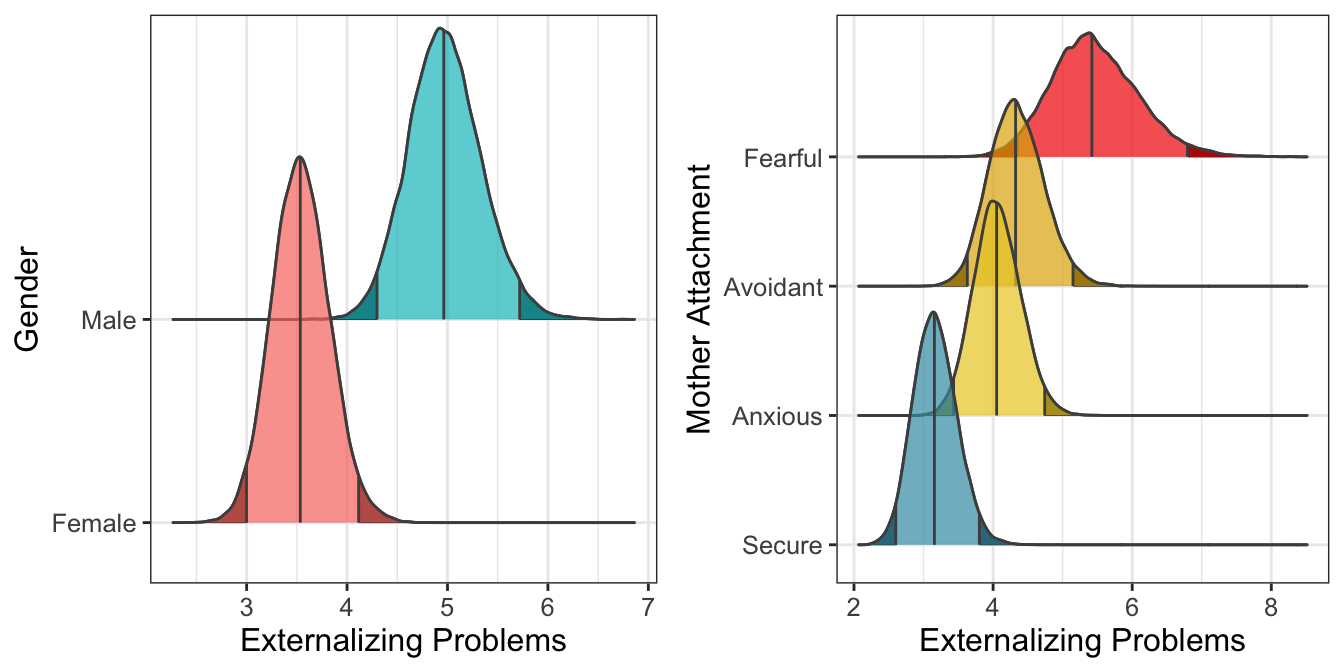
\includegraphics[width=0.95\linewidth]{attachment-bayes-factor_files/figure-latex/plot-marginal-ext-1} 

}

\caption{Marginal predicted values according to gender and mother attachment ($n_{subj} = 847$).}\label{fig:plot-marginal-ext}
\end{figure}

\begin{figure}

{\centering 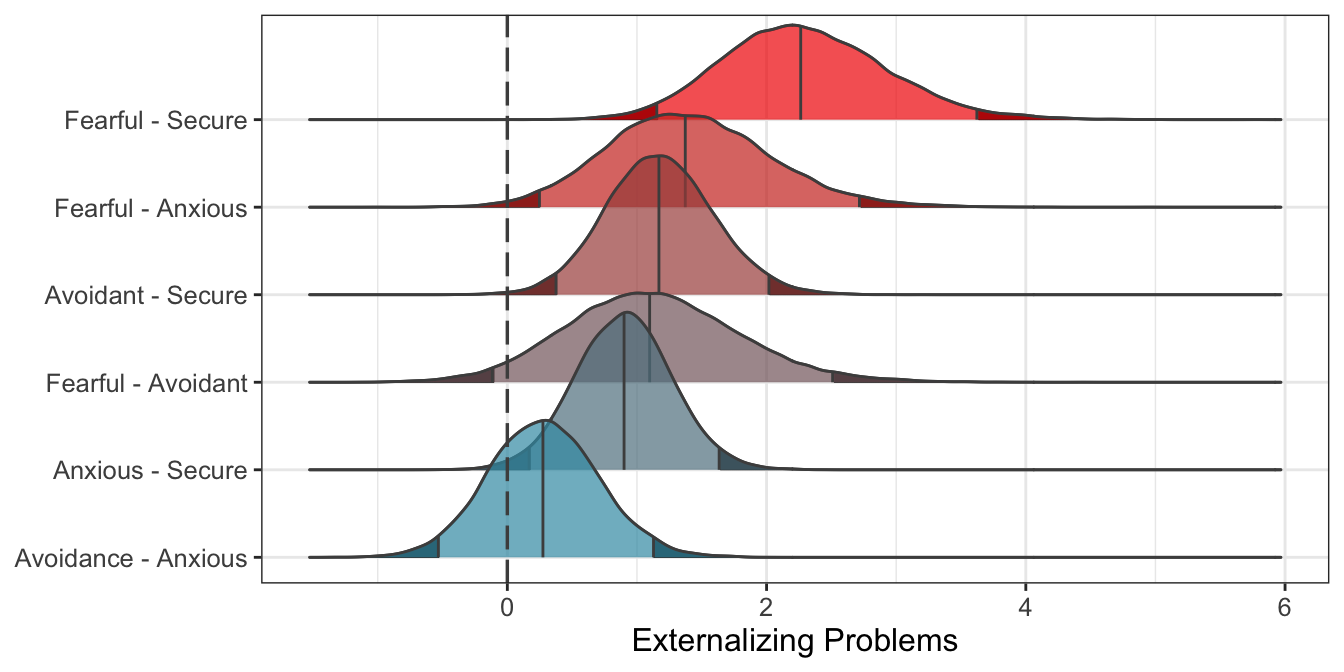
\includegraphics{attachment-bayes-factor_files/figure-latex/plot-diff-ext-1} 

}

\caption{Predicted differences between mother attachment patterns ($n_{subj} = 847$).}\label{fig:plot-diff-ext}
\end{figure}

Overall, results indicate that Males have more externalizing problems than Females. Regarding mother attachment, Fearful, Avoidant, and Anxious children have more problems than Secure children. Moreover, Fearful children have more problems than Anxious children.

To evaluate the fit of the model to the data, we computed the \emph{Bayesian} \(R^2\), using the function \texttt{brms::bayes\_R2()}, and we present Posterior Predictions in Figure\textasciitilde\ref{fig:plot-ppcheck-ext}.

\begin{Shaded}
\begin{Highlighting}[]
\NormalTok{r2\_ext}
\DocumentationTok{\#\#     Estimate  Est.Error       Q2.5     Q97.5}
\DocumentationTok{\#\# R2 0.1484309 0.02931432 0.09501877 0.2107168}
\end{Highlighting}
\end{Shaded}

\begin{verbatim}
## Warning: Argument 'nsamples' is deprecated. Please use argument 'ndraws' instead.
\end{verbatim}

\begin{figure}

{\centering 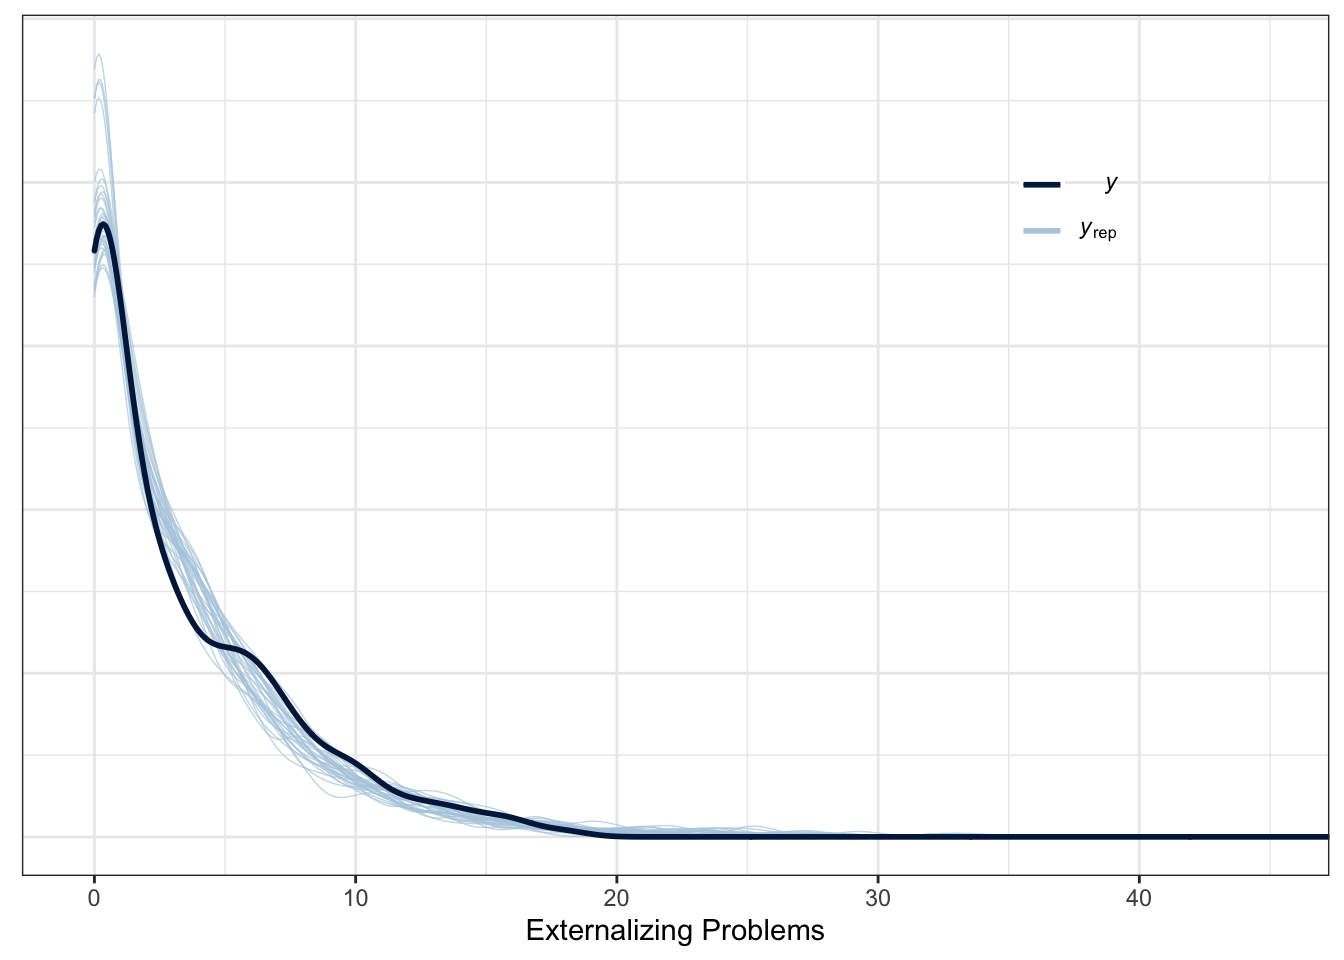
\includegraphics{attachment-bayes-factor_files/figure-latex/plot-ppcheck-ext-1} 

}

\caption{Posterior predictive check ($n_{subj} = 847$).}\label{fig:plot-ppcheck-ext}
\end{figure}

We can see that the actual variance explained by fixed effects and random effects is around 15\%. Moreover, the posterior predictive check indicates a good fit to the data.

\hypertarget{conclusions-2}{%
\subsubsection*{Conclusions}\label{conclusions-2}}
\addcontentsline{toc}{subsubsection}{Conclusions}

Considering attachment theoretical perspectives, results indicate only the role of mother attachment so we can support the Monotropy Theory.

\hypertarget{conclusion-ext}{%
\chapter{Conclusions}\label{conclusion-ext}}

Overall, we obtained consistent results from the three different approaches. Males have more problems than Females and, regarding attachment, only mother attachment influences children's externalizing problems. In particular, we observed the following pattern: Secure children have the lowest level of problems, Anxious and Avoidant children have a similar, intermediate, level of problems, and Fearful children have the highest level of problems. Taken together, these results support the Monotropy Theory.

Although if the different approaches lead to apparently similar results, the rigorous interpretation of the results is very different.

\begin{itemize}
\tightlist
\item
  Considering the NHST approach, we actually only found that it is unlikely that mother attachment has no effect. Thus, we reject the null hypothesis but we can not quantify the evidence in favour of any of our hypotheses.
\item
  Only model comparison allows us to quantify the relative evidence of our models. Model comparison results clearly indicated evidence in favour of an effect of mother attachment but not father attachment. However, using information criteria we could not directly evaluate our informative hypotheses regarding the expected effects, but only the presence of any effect.
\item
  Bayes factor with encompassing prior approach allowed us to directly test our informative hypotheses regarding the expected effects. Results clearly selected the Monotropy theory as the most likely theory among those considered.
\end{itemize}

To summarize, the apparently identical results actually have a completely different meaning and what we learn from the data is very different. Hopefully, now it is clear that statistical inference is a complex process that requires careful thinking. In particular, to answer the questions we are actually interested in, we need to apply the appropriate statistical techniques.

\hypertarget{part-internalizing-problems}{%
\part*{Internalizing Problems}\label{part-internalizing-problems}}
\addcontentsline{toc}{part}{Internalizing Problems}

\hypertarget{model-choice-int}{%
\chapter{Models Family Choice}\label{model-choice-int}}

In this chapter, we discuss the appropriate models' family to take into account data characteristics.

Internalizing problems are computed as the sum of 10 items of the SDQ, obtaining discrete scores that range from 0 to 20. Considering data distribution (see Figure\textasciitilde\ref{fig:plot-internalizing-dist}), we choose a \textbf{Negative Binomial} distribution to model the data.

\hypertarget{zero-inflated-negative-binomial-1}{%
\section{Zero Inflated Negative Binomial}\label{zero-inflated-negative-binomial-1}}

As in the case of externalizing problems, we evaluate whether a \emph{Zero-Inflated} model may be appropriate. We compare the number of observed zeros and expected zeros in a Negative Binomial mixed-effects model considering the same predictors as in the case of externalizing problems. Using R formula syntax, we have

\begin{Shaded}
\begin{Highlighting}[]
\CommentTok{\# model formula}
\NormalTok{internalizing\_sum }\SpecialCharTok{\textasciitilde{}}\NormalTok{ gender }\SpecialCharTok{+}\NormalTok{ mother }\SpecialCharTok{*}\NormalTok{ father }\SpecialCharTok{+}\NormalTok{ (}\DecValTok{1}\SpecialCharTok{|}\NormalTok{ID\_class)}
\end{Highlighting}
\end{Shaded}

Comparing the number of observed zero and expected zeros, we get

\begin{Shaded}
\begin{Highlighting}[]
\FunctionTok{my\_check\_zeroinflation}\NormalTok{(fit\_int\_nb)}
\DocumentationTok{\#\# \# Check for zero{-}inflation}
\DocumentationTok{\#\# }
\DocumentationTok{\#\#    Observed zeros: 226}
\DocumentationTok{\#\#   Predicted zeros: 195}
\DocumentationTok{\#\#             Ratio: 0.86}
\DocumentationTok{\#\# Model is underfitting zeros (probable zero{-}inflation).}
\end{Highlighting}
\end{Shaded}

Results indicate that the model is slightly under-fitting the number of zeros. Thus, we can fit a \emph{Zero Inflated Negative Binomial} (ZINB) model and compare the performance of the two models. Using R formula syntax, we have

\begin{Shaded}
\begin{Highlighting}[]
\CommentTok{\# formula for p}
\NormalTok{p }\SpecialCharTok{\textasciitilde{}}\NormalTok{ gender }\SpecialCharTok{+}\NormalTok{ (}\DecValTok{1}\SpecialCharTok{|}\NormalTok{ID\_class)}

\CommentTok{\# formula for mu}
\NormalTok{mu }\SpecialCharTok{\textasciitilde{}}\NormalTok{ gender }\SpecialCharTok{+}\NormalTok{ mother }\SpecialCharTok{*}\NormalTok{ father }\SpecialCharTok{+}\NormalTok{ (}\DecValTok{1}\SpecialCharTok{|}\NormalTok{ID\_class)}
\end{Highlighting}
\end{Shaded}

Below we report results of the analysis of deviance.

\begin{Shaded}
\begin{Highlighting}[]
\FunctionTok{anova}\NormalTok{(fit\_int\_nb, fit\_int\_zinb)}
\DocumentationTok{\#\# Data: data\_cluster}
\DocumentationTok{\#\# Models:}
\DocumentationTok{\#\# fit\_int\_nb: internalizing\_sum \textasciitilde{} gender + mother * father + (1 | ID\_class), zi=\textasciitilde{}0, disp=\textasciitilde{}1}
\DocumentationTok{\#\# fit\_int\_zinb: internalizing\_sum \textasciitilde{} gender + mother * father + (1 | ID\_class), zi=\textasciitilde{}gender + (1 | ID\_class), disp=\textasciitilde{}1}
\DocumentationTok{\#\#              Df    AIC    BIC  logLik deviance  Chisq Chi Df Pr(\textgreater{}Chisq)    }
\DocumentationTok{\#\# fit\_int\_nb   19 3680.7 3770.8 {-}1821.3   3642.7                             }
\DocumentationTok{\#\# fit\_int\_zinb 22 3669.0 3773.3 {-}1812.5   3625.0 17.677      3  0.0005127 ***}
\DocumentationTok{\#\# {-}{-}{-}}
\DocumentationTok{\#\# Signif. codes:  0 \textquotesingle{}***\textquotesingle{} 0.001 \textquotesingle{}**\textquotesingle{} 0.01 \textquotesingle{}*\textquotesingle{} 0.05 \textquotesingle{}.\textquotesingle{} 0.1 \textquotesingle{} \textquotesingle{} 1}
\end{Highlighting}
\end{Shaded}

Overall, results indicate that the ZINB model performs better than the Negative Binomial model. Note, however, that BIC actually prefers the model without zero inflation. Nevertheless, in the following analyses, we decide to use ZINB models to be consistent with the analysis of the externalizing problems.

\hypertarget{nhst-int}{%
\chapter{NHST}\label{nhst-int}}

Following the traditional NHST approach, we consider the model previously defined that includes all effects of interest (gender effect and the interaction between mother attachment and father attachment). Results of the analysis of deviance are reported below.

\begin{Shaded}
\begin{Highlighting}[]
\NormalTok{car}\SpecialCharTok{::}\FunctionTok{Anova}\NormalTok{(fit\_int\_zinb)}
\DocumentationTok{\#\# Analysis of Deviance Table (Type II Wald chisquare tests)}
\DocumentationTok{\#\# }
\DocumentationTok{\#\# Response: internalizing\_sum}
\DocumentationTok{\#\#                 Chisq Df Pr(\textgreater{}Chisq)   }
\DocumentationTok{\#\# gender         0.9449  1   0.331015   }
\DocumentationTok{\#\# mother        12.4302  3   0.006046 **}
\DocumentationTok{\#\# father         2.6855  3   0.442698   }
\DocumentationTok{\#\# mother:father  9.6213  9   0.382006   }
\DocumentationTok{\#\# {-}{-}{-}}
\DocumentationTok{\#\# Signif. codes:  0 \textquotesingle{}***\textquotesingle{} 0.001 \textquotesingle{}**\textquotesingle{} 0.01 \textquotesingle{}*\textquotesingle{} 0.05 \textquotesingle{}.\textquotesingle{} 0.1 \textquotesingle{} \textquotesingle{} 1}
\end{Highlighting}
\end{Shaded}

Results indicate only a statistically significant effect of mother attachment. On the contrary, the interaction and father attachment are not significant. The model summary is reported below.

\begin{Shaded}
\begin{Highlighting}[]
\FunctionTok{summary}\NormalTok{(fit\_int\_zinb)}
\DocumentationTok{\#\#  Family: nbinom2  ( log )}
\DocumentationTok{\#\# Formula:          internalizing\_sum \textasciitilde{} gender + mother * father + (1 | ID\_class)}
\DocumentationTok{\#\# Zero inflation:                     \textasciitilde{}gender + (1 | ID\_class)}
\DocumentationTok{\#\# Data: data\_cluster}
\DocumentationTok{\#\# }
\DocumentationTok{\#\#      AIC      BIC   logLik deviance df.resid }
\DocumentationTok{\#\#   3669.0   3773.3  {-}1812.5   3625.0      825 }
\DocumentationTok{\#\# }
\DocumentationTok{\#\# Random effects:}
\DocumentationTok{\#\# }
\DocumentationTok{\#\# Conditional model:}
\DocumentationTok{\#\#  Groups   Name        Variance Std.Dev.}
\DocumentationTok{\#\#  ID\_class (Intercept) 0.1364   0.3693  }
\DocumentationTok{\#\# Number of obs: 847, groups:  ID\_class, 50}
\DocumentationTok{\#\# }
\DocumentationTok{\#\# Zero{-}inflation model:}
\DocumentationTok{\#\#  Groups   Name        Variance Std.Dev.}
\DocumentationTok{\#\#  ID\_class (Intercept) 3.225    1.796   }
\DocumentationTok{\#\# Number of obs: 847, groups:  ID\_class, 50}
\DocumentationTok{\#\# }
\DocumentationTok{\#\# Dispersion parameter for nbinom2 family ():  2.6 }
\DocumentationTok{\#\# }
\DocumentationTok{\#\# Conditional model:}
\DocumentationTok{\#\#                               Estimate Std. Error z value Pr(\textgreater{}|z|)    }
\DocumentationTok{\#\# (Intercept)                    0.85592    0.12115   7.065 1.61e{-}12 ***}
\DocumentationTok{\#\# genderM                        0.06854    0.07051   0.972  0.33101    }
\DocumentationTok{\#\# motherAnxious                  0.47960    0.16672   2.877  0.00402 ** }
\DocumentationTok{\#\# motherAvoidant                {-}0.08057    0.24671  {-}0.327  0.74398    }
\DocumentationTok{\#\# motherFearful                  0.66801    0.41101   1.625  0.10410    }
\DocumentationTok{\#\# fatherAnxious                  0.07410    0.16668   0.445  0.65661    }
\DocumentationTok{\#\# fatherAvoidant                 0.09901    0.17349   0.571  0.56822    }
\DocumentationTok{\#\# fatherFearful                  0.38182    0.33578   1.137  0.25550    }
\DocumentationTok{\#\# motherAnxious:fatherAnxious   {-}0.26373    0.23441  {-}1.125  0.26055    }
\DocumentationTok{\#\# motherAvoidant:fatherAnxious   0.25023    0.30643   0.817  0.41416    }
\DocumentationTok{\#\# motherFearful:fatherAnxious   {-}0.80565    0.50634  {-}1.591  0.11158    }
\DocumentationTok{\#\# motherAnxious:fatherAvoidant  {-}0.25807    0.23926  {-}1.079  0.28076    }
\DocumentationTok{\#\# motherAvoidant:fatherAvoidant  0.10204    0.30109   0.339  0.73467    }
\DocumentationTok{\#\# motherFearful:fatherAvoidant  {-}0.25422    0.46295  {-}0.549  0.58292    }
\DocumentationTok{\#\# motherAnxious:fatherFearful   {-}0.53674    0.39927  {-}1.344  0.17885    }
\DocumentationTok{\#\# motherAvoidant:fatherFearful   0.23131    0.47623   0.486  0.62718    }
\DocumentationTok{\#\# motherFearful:fatherFearful   {-}0.41834    0.54125  {-}0.773  0.43958    }
\DocumentationTok{\#\# {-}{-}{-}}
\DocumentationTok{\#\# Signif. codes:  0 \textquotesingle{}***\textquotesingle{} 0.001 \textquotesingle{}**\textquotesingle{} 0.01 \textquotesingle{}*\textquotesingle{} 0.05 \textquotesingle{}.\textquotesingle{} 0.1 \textquotesingle{} \textquotesingle{} 1}
\DocumentationTok{\#\# }
\DocumentationTok{\#\# Zero{-}inflation model:}
\DocumentationTok{\#\#             Estimate Std. Error z value Pr(\textgreater{}|z|)    }
\DocumentationTok{\#\# (Intercept)  {-}2.6112     0.6183  {-}4.223 2.41e{-}05 ***}
\DocumentationTok{\#\# genderM      {-}0.2890     0.3531  {-}0.818    0.413    }
\DocumentationTok{\#\# {-}{-}{-}}
\DocumentationTok{\#\# Signif. codes:  0 \textquotesingle{}***\textquotesingle{} 0.001 \textquotesingle{}**\textquotesingle{} 0.01 \textquotesingle{}*\textquotesingle{} 0.05 \textquotesingle{}.\textquotesingle{} 0.1 \textquotesingle{} \textquotesingle{} 1}
\end{Highlighting}
\end{Shaded}

To evaluate the effect of mother attachment, the marginal predicted values are presented in Figure\textasciitilde\ref{fig:plot-nhst-effects-int}. Note that the marginal predicted values are averaged over father attachment and gender effect.

\begin{figure}

{\centering 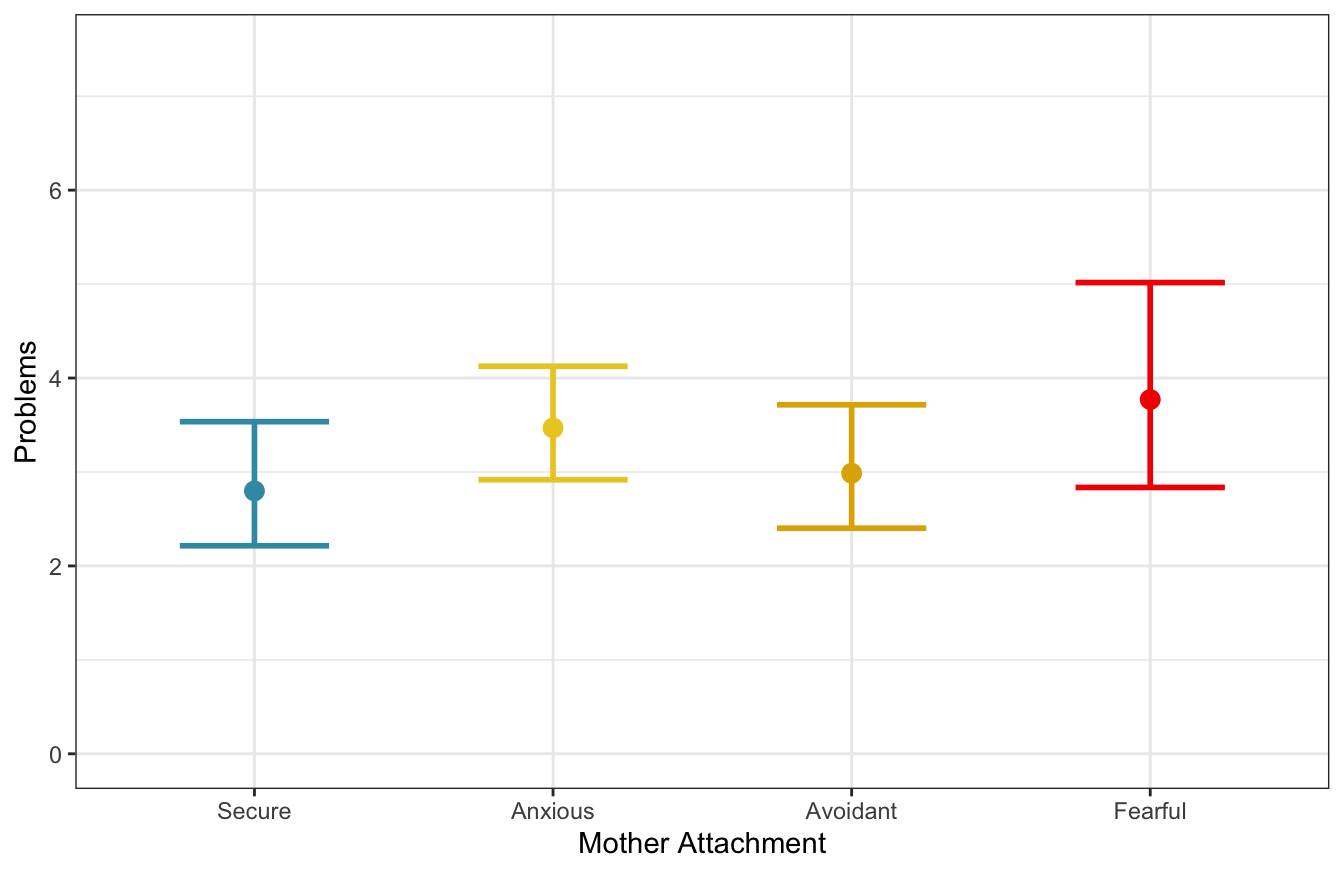
\includegraphics{attachment-bayes-factor_files/figure-latex/plot-nhst-effects-int-1} 

}

\caption{Marginal predicted values according to mother attachment. Values are averaged over the other effects ($n_{subj} = 847$).}\label{fig:plot-nhst-effects-int}
\end{figure}

Post-hoc tests are run to evaluate differences between mother attachment styles, considering pairwise comparisons and adjusting \emph{p}-values according to multivariate \emph{t}-distribution. Results are reported below,

\begin{Shaded}
\begin{Highlighting}[]
\NormalTok{emmeans}\SpecialCharTok{::}\FunctionTok{contrast}\NormalTok{(emmeans}\SpecialCharTok{::}\FunctionTok{emmeans}\NormalTok{(fit\_int\_zinb, }\AttributeTok{specs =} \SpecialCharTok{\textasciitilde{}}\NormalTok{ mother ),}
                  \StringTok{"pairwise"}\NormalTok{, }\AttributeTok{adjust =} \StringTok{"mvt"}\NormalTok{)}
\DocumentationTok{\#\# }\AlertTok{NOTE}\DocumentationTok{: Results may be misleading due to involvement in interactions}
\DocumentationTok{\#\#  contrast           estimate    SE  df t.ratio p.value}
\DocumentationTok{\#\#  Secure {-} Anxious    {-}0.2150 0.117 825  {-}1.836  0.2510}
\DocumentationTok{\#\#  Secure {-} Avoidant   {-}0.0653 0.136 825  {-}0.481  0.9622}
\DocumentationTok{\#\#  Secure {-} Fearful    {-}0.2985 0.166 825  {-}1.793  0.2708}
\DocumentationTok{\#\#  Anxious {-} Avoidant   0.1496 0.112 825   1.336  0.5321}
\DocumentationTok{\#\#  Anxious {-} Fearful   {-}0.0835 0.147 825  {-}0.566  0.9403}
\DocumentationTok{\#\#  Avoidant {-} Fearful  {-}0.2331 0.164 825  {-}1.423  0.4774}
\DocumentationTok{\#\# }
\DocumentationTok{\#\# Results are averaged over the levels of: gender, father }
\DocumentationTok{\#\# Results are given on the log (not the response) scale. }
\DocumentationTok{\#\# P value adjustment: mvt method for 6 tests}
\end{Highlighting}
\end{Shaded}

After adjusting p-values we actually get that there are no statistically significant differences. Without adjusting, the difference between Anxious and Secure children and the difference between Fearful and Secure children have a low (but not statistically significant) \emph{p}-value.

\begin{Shaded}
\begin{Highlighting}[]
\NormalTok{emmeans}\SpecialCharTok{::}\FunctionTok{contrast}\NormalTok{(emmeans}\SpecialCharTok{::}\FunctionTok{emmeans}\NormalTok{(fit\_int\_zinb, }\AttributeTok{specs =} \SpecialCharTok{\textasciitilde{}}\NormalTok{ mother ),}
                  \StringTok{"pairwise"}\NormalTok{, }\AttributeTok{adjust =} \ConstantTok{NULL}\NormalTok{)}
\DocumentationTok{\#\# }\AlertTok{NOTE}\DocumentationTok{: Results may be misleading due to involvement in interactions}
\DocumentationTok{\#\#  contrast           estimate    SE  df t.ratio p.value}
\DocumentationTok{\#\#  Secure {-} Anxious    {-}0.2150 0.117 825  {-}1.836  0.0668}
\DocumentationTok{\#\#  Secure {-} Avoidant   {-}0.0653 0.136 825  {-}0.481  0.6307}
\DocumentationTok{\#\#  Secure {-} Fearful    {-}0.2985 0.166 825  {-}1.793  0.0734}
\DocumentationTok{\#\#  Anxious {-} Avoidant   0.1496 0.112 825   1.336  0.1818}
\DocumentationTok{\#\#  Anxious {-} Fearful   {-}0.0835 0.147 825  {-}0.566  0.5713}
\DocumentationTok{\#\#  Avoidant {-} Fearful  {-}0.2331 0.164 825  {-}1.423  0.1551}
\DocumentationTok{\#\# }
\DocumentationTok{\#\# Results are averaged over the levels of: gender, father }
\DocumentationTok{\#\# Results are given on the log (not the response) scale.}
\end{Highlighting}
\end{Shaded}

To evaluate the fit of the model to the data, we computed the \emph{Marginal} \(R^2\) and the \emph{Conditional} \(R^2\).

\begin{Shaded}
\begin{Highlighting}[]
\NormalTok{performance}\SpecialCharTok{::}\FunctionTok{r2}\NormalTok{(fit\_int\_zinb)}
\DocumentationTok{\#\# Warning: mu of 3.2 is too close to zero, estimate of random effect variances may be unreliable.}
\DocumentationTok{\#\# \# R2 for Mixed Models}
\DocumentationTok{\#\# }
\DocumentationTok{\#\#   Conditional R2: 0.217}
\DocumentationTok{\#\#      Marginal R2: 0.047}
\end{Highlighting}
\end{Shaded}

We can see that the actual variance explained by fixed effects is less than 5\%, not that much.

\hypertarget{conclusions-3}{%
\subsubsection*{Conclusions}\label{conclusions-3}}
\addcontentsline{toc}{subsubsection}{Conclusions}

Results are difficult to interpret because we have a statistically significant effect of mother attachment, but, considering pot-hoc tests, we get no statistically significant difference.
Overall, we could say that, in some way, results indicate a role of mother attachment but this probably is small.

\hypertarget{model-comparison-int}{%
\chapter{Model Comparison}\label{model-comparison-int}}

\hypertarget{formalize-models-1}{%
\section{Formalize Models}\label{formalize-models-1}}

We consider Zero Inflated Negative Binomial Mixed-Effects models with only the role of gender as a fixed effect and children's classroom ID as a random effect for \(p\). Whereas, considering \(\mu\), we define the same models as in the analysis of externalizing problems. Using R formula syntax, we have

\begin{Shaded}
\begin{Highlighting}[]
\CommentTok{\# formula for p (same for all models)}
\NormalTok{p }\SpecialCharTok{\textasciitilde{}}\NormalTok{ gender }\SpecialCharTok{+}\NormalTok{ (}\DecValTok{1}\SpecialCharTok{|}\NormalTok{ID\_class)}

\CommentTok{\# formula for mu}

\CommentTok{\# fit\_int\_zero}
\NormalTok{mu }\SpecialCharTok{\textasciitilde{}}\NormalTok{ gender }\SpecialCharTok{+}\NormalTok{ (}\DecValTok{1}\SpecialCharTok{|}\NormalTok{ID\_class)}

\CommentTok{\# fit\_int\_mother}
\NormalTok{mu }\SpecialCharTok{\textasciitilde{}}\NormalTok{ gender }\SpecialCharTok{+}\NormalTok{ mother }\SpecialCharTok{+}\NormalTok{ (}\DecValTok{1}\SpecialCharTok{|}\NormalTok{ID\_class)}

\CommentTok{\# fit\_int\_additive}
\NormalTok{mu }\SpecialCharTok{\textasciitilde{}}\NormalTok{ gender }\SpecialCharTok{+}\NormalTok{ mother }\SpecialCharTok{+}\NormalTok{ father }\SpecialCharTok{+}\NormalTok{ (}\DecValTok{1}\SpecialCharTok{|}\NormalTok{ID\_class)}

\CommentTok{\# fit\_int\_inter}
\NormalTok{mu }\SpecialCharTok{\textasciitilde{}}\NormalTok{ gender }\SpecialCharTok{+}\NormalTok{ mother }\SpecialCharTok{*}\NormalTok{ father }\SpecialCharTok{+}\NormalTok{ (}\DecValTok{1}\SpecialCharTok{|}\NormalTok{ID\_class)}
\end{Highlighting}
\end{Shaded}

\hypertarget{aic-and-bic-results-1}{%
\section{AIC and BIC Results}\label{aic-and-bic-results-1}}

AIC and BIC values together with their relative weights are computed and reported in Table\textasciitilde\ref{tab:table-AIC-BIC-weights-int}.

\begin{table}[!h]

\caption{\label{tab:table-AIC-BIC-weights-int}Model comparison internalizing problems ($n_{subj} = 847$).}
\centering
\resizebox{\linewidth}{!}{
\begin{tabular}[t]{rccc>{\centering\arraybackslash}m{1cm}cc>{\centering\arraybackslash}m{1cm}}
\toprule
\textbf{Model} & \textbf{Df} & \textbf{AIC} & \textbf{AIC$_{weights}$} & \textbf{ } & \textbf{BIC} & \textbf{BIC$_{weights}$} & \textbf{ }\\
\midrule
fit-int-zero & 6 & 3671.4 & 0.00 & 
\includegraphics[width=0.33in, height=0.33in]{images/ball_AIC_int_zero.png} & 3704.6 & 0.52 & 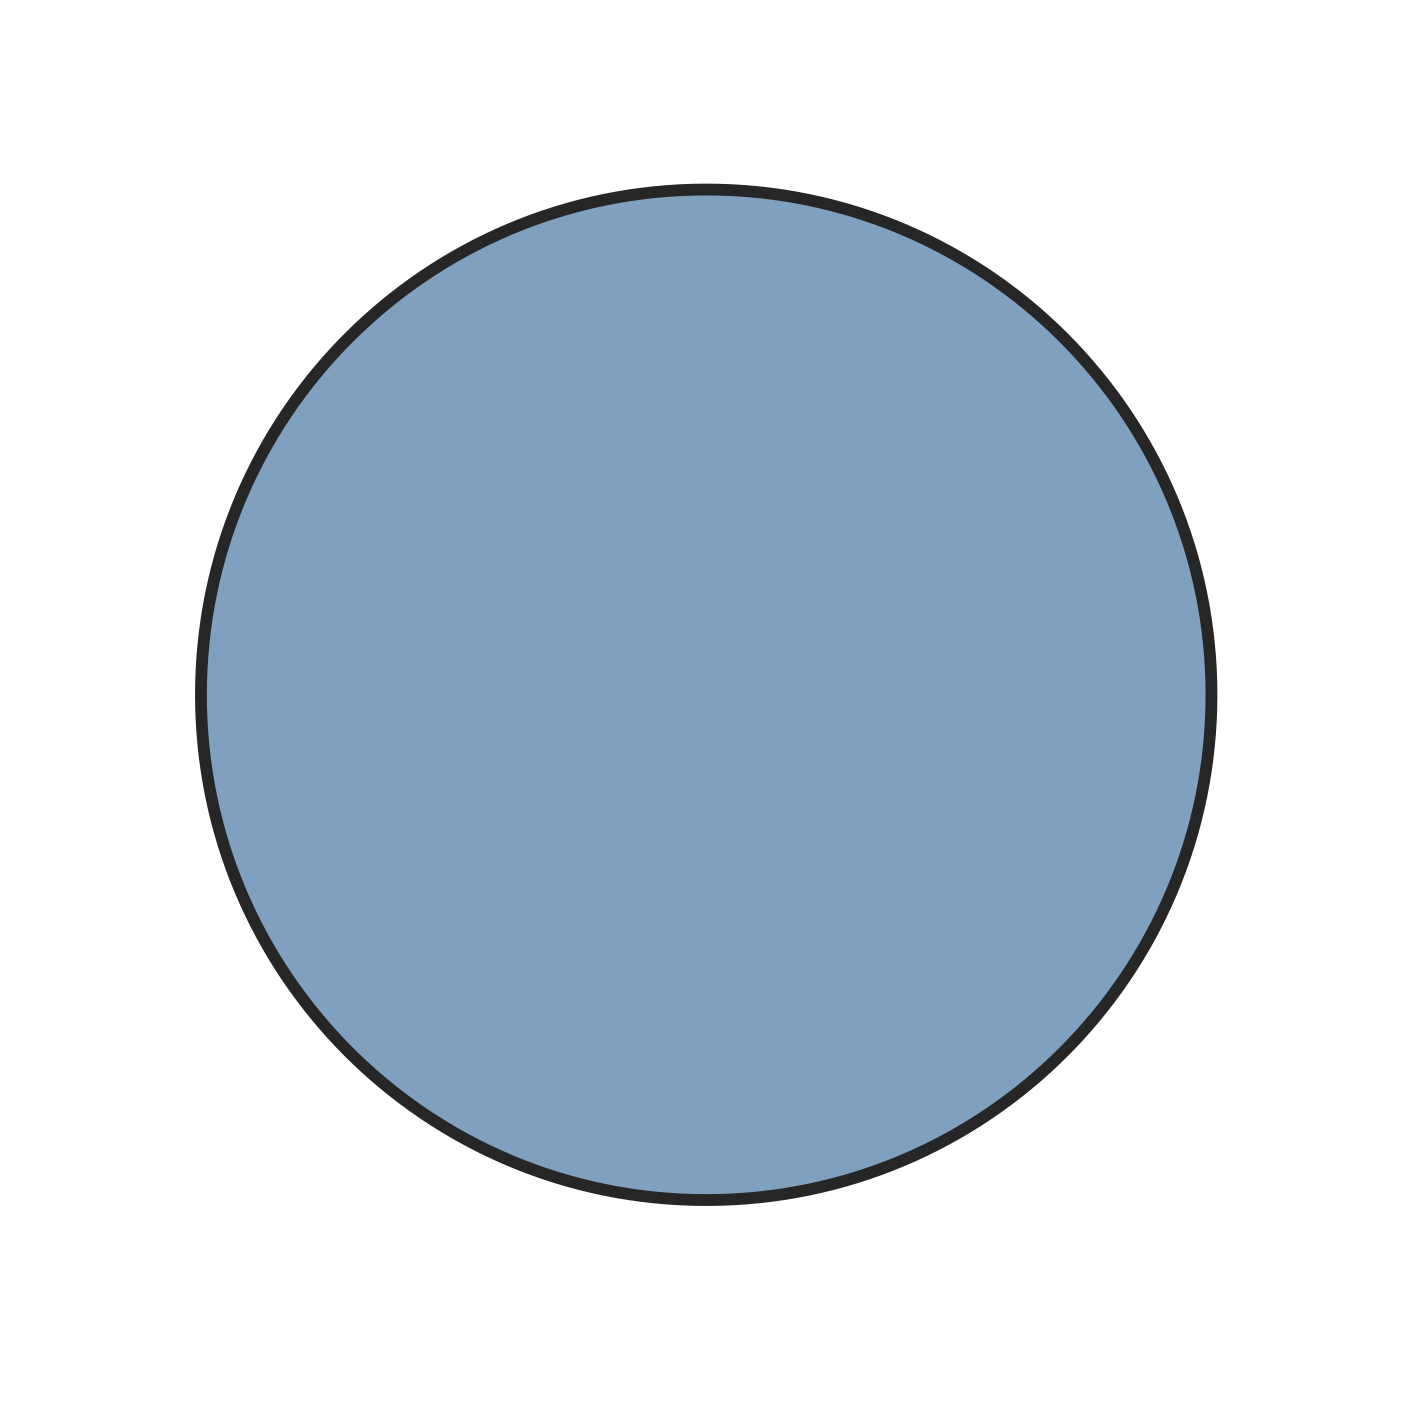
\includegraphics[width=0.33in, height=0.33in]{images/ball_BIC_int_zero.png}\\
fit-int-mother & 9 & 3657.4 & 0.83 & 
\includegraphics[width=0.33in, height=0.33in]{images/ball_AIC_int_mother.png} & 3704.8 & 0.48 & 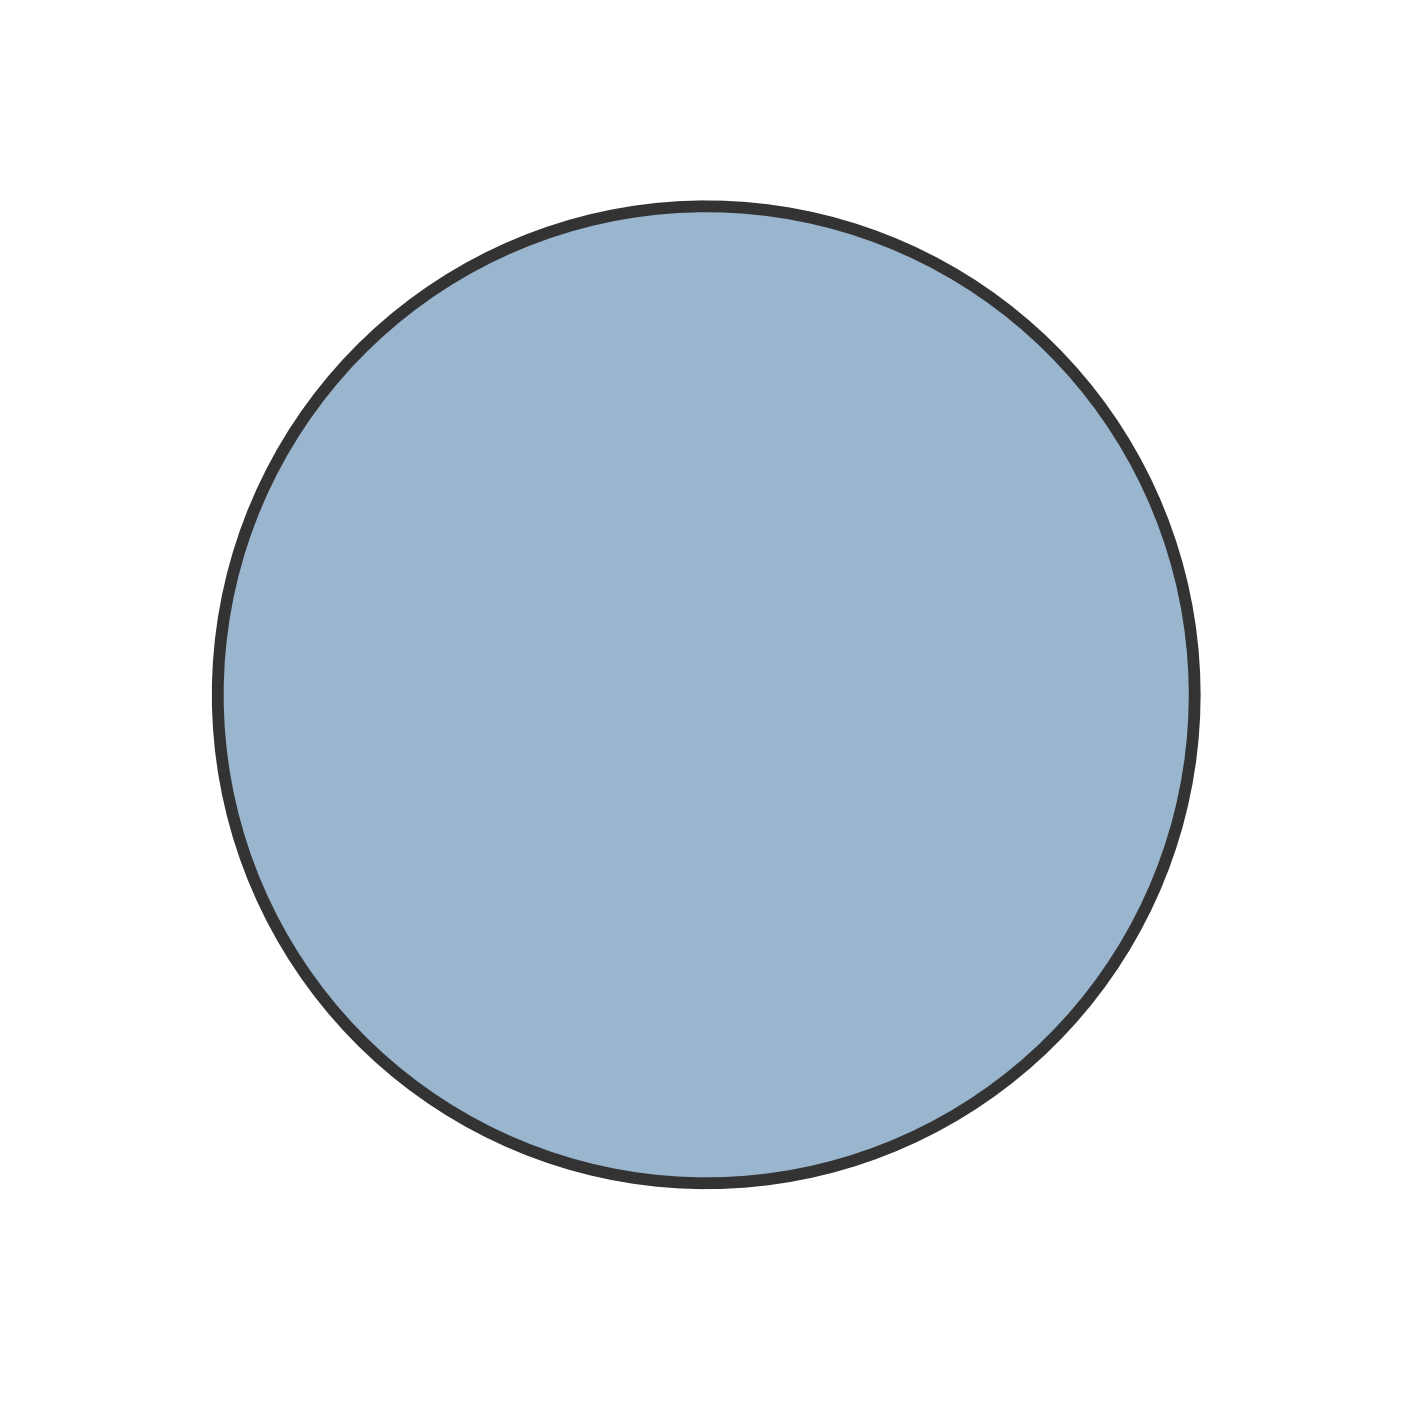
\includegraphics[width=0.33in, height=0.33in]{images/ball_BIC_int_mother.png}\\
fit-int-additive & 12 & 3660.6 & 0.16 & 
\includegraphics[width=0.33in, height=0.33in]{images/ball_AIC_int_additive.png} & 3722.2 & 0.00 & 
\includegraphics[width=0.33in, height=0.33in]{images/ball_BIC_int_additive.png}\\
fit-int-inter & 21 & 3669.0 & 0.00 & 
\includegraphics[width=0.33in, height=0.33in]{images/ball_AIC_int_inter.png} & 3773.3 & 0.00 & 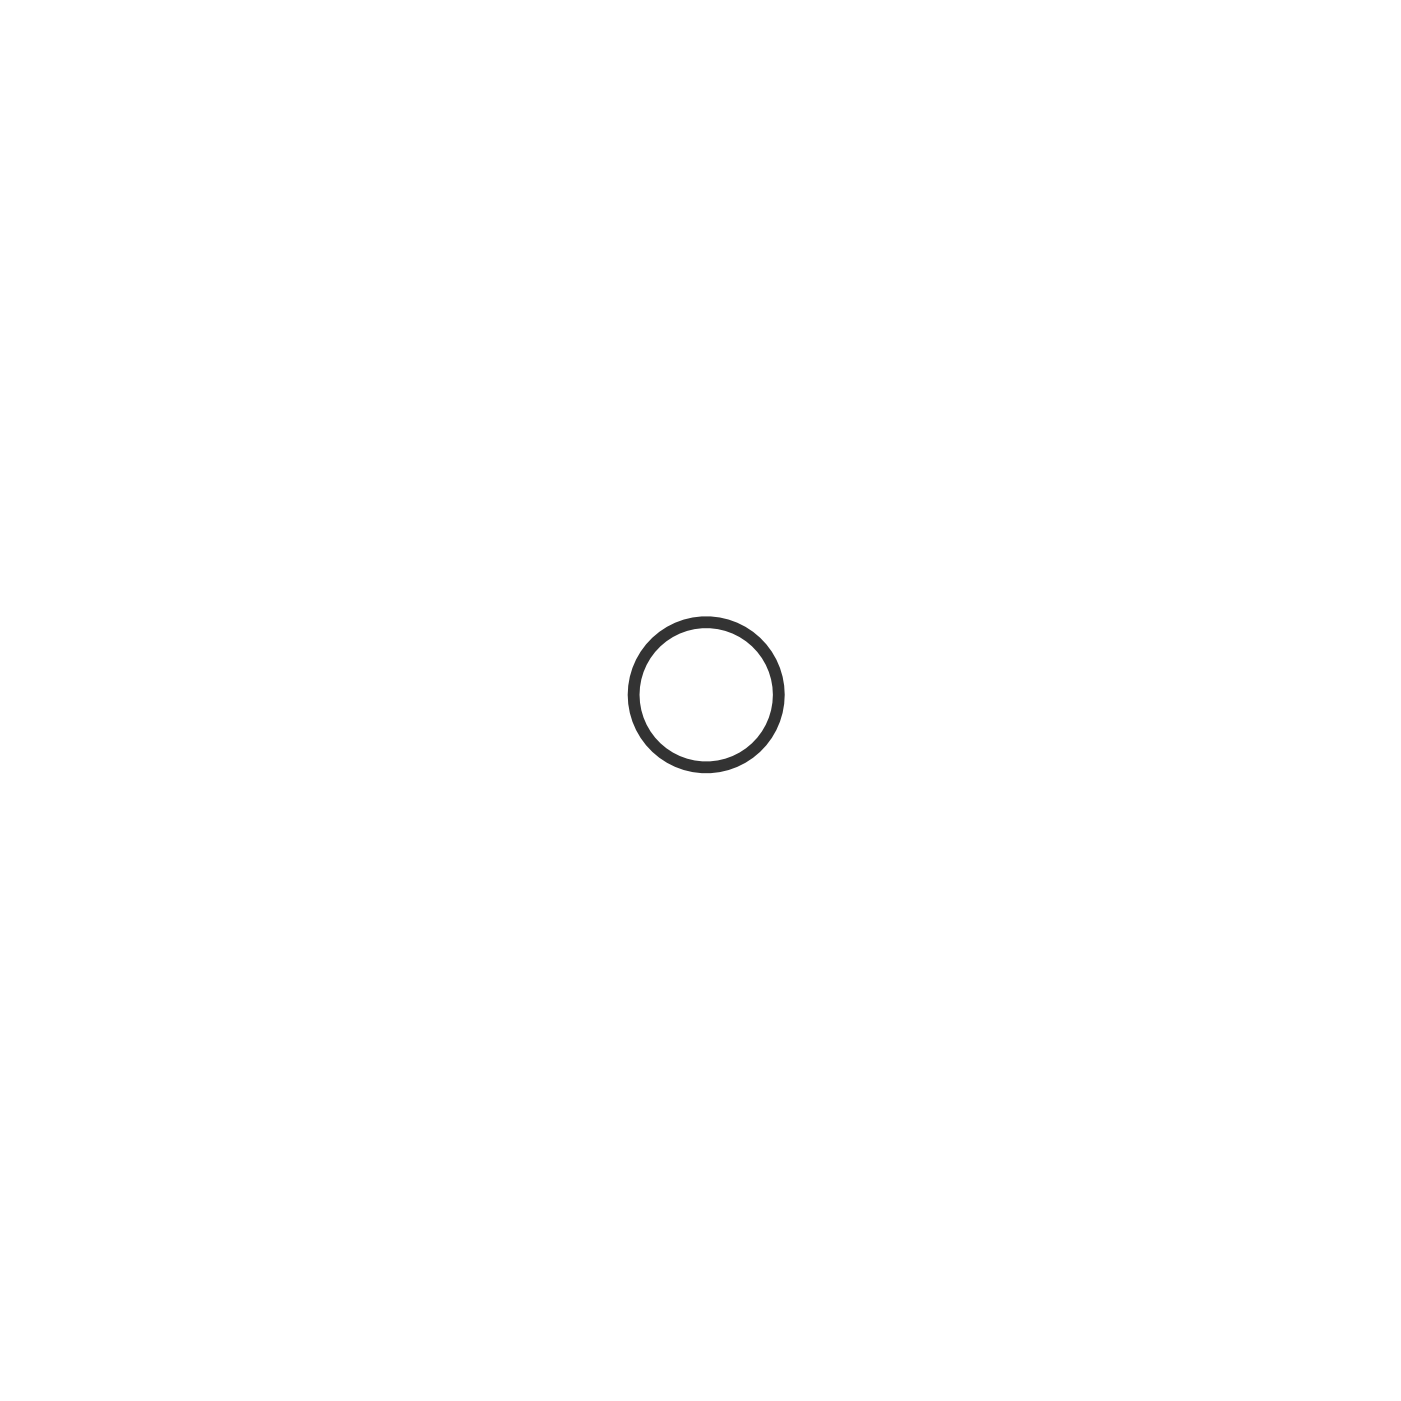
\includegraphics[width=0.33in, height=0.33in]{images/ball_BIC_int_inter.png}\\
\bottomrule
\end{tabular}}
\end{table}

According to AIC, the most likely model is \texttt{fit\_int\_mother} (83\%) and the second most likely model is \texttt{fit\_int\_additive} (16\%) given the data and the set of models considered. According to BIC, instead, \texttt{fit\_int\_zero} and \texttt{fit\_int\_mother} models have almost the same probability, 52\% and 48\% respectively.

We can say that there is evidence in favour of the role of mother attachment but probably this effect is small.

\hypertarget{selected-model-2}{%
\section{Selected Model}\label{selected-model-2}}

Results of analysis of deviance for model \texttt{fit\_int\_mother} are reported below.

\begin{Shaded}
\begin{Highlighting}[]
\NormalTok{car}\SpecialCharTok{::}\FunctionTok{Anova}\NormalTok{(fit\_int\_mother)}
\DocumentationTok{\#\# Analysis of Deviance Table (Type II Wald chisquare tests)}
\DocumentationTok{\#\# }
\DocumentationTok{\#\# Response: internalizing\_sum}
\DocumentationTok{\#\#         Chisq Df Pr(\textgreater{}Chisq)    }
\DocumentationTok{\#\# gender  0.754  1  0.3852261    }
\DocumentationTok{\#\# mother 19.894  3  0.0001786 ***}
\DocumentationTok{\#\# {-}{-}{-}}
\DocumentationTok{\#\# Signif. codes:  0 \textquotesingle{}***\textquotesingle{} 0.001 \textquotesingle{}**\textquotesingle{} 0.01 \textquotesingle{}*\textquotesingle{} 0.05 \textquotesingle{}.\textquotesingle{} 0.1 \textquotesingle{} \textquotesingle{} 1}
\end{Highlighting}
\end{Shaded}

Results confirm a statistically significant effect of mother attachment. The model summary is reported below.

\begin{Shaded}
\begin{Highlighting}[]
\FunctionTok{summary}\NormalTok{(fit\_int\_mother)}
\DocumentationTok{\#\#  Family: nbinom2  ( log )}
\DocumentationTok{\#\# Formula:          internalizing\_sum \textasciitilde{} gender + mother + (1 | ID\_class)}
\DocumentationTok{\#\# Zero inflation:                     \textasciitilde{}gender + (1 | ID\_class)}
\DocumentationTok{\#\# Data: data\_cluster}
\DocumentationTok{\#\# }
\DocumentationTok{\#\#      AIC      BIC   logLik deviance df.resid }
\DocumentationTok{\#\#   3657.4   3704.8  {-}1818.7   3637.4      837 }
\DocumentationTok{\#\# }
\DocumentationTok{\#\# Random effects:}
\DocumentationTok{\#\# }
\DocumentationTok{\#\# Conditional model:}
\DocumentationTok{\#\#  Groups   Name        Variance Std.Dev.}
\DocumentationTok{\#\#  ID\_class (Intercept) 0.1423   0.3772  }
\DocumentationTok{\#\# Number of obs: 847, groups:  ID\_class, 50}
\DocumentationTok{\#\# }
\DocumentationTok{\#\# Zero{-}inflation model:}
\DocumentationTok{\#\#  Groups   Name        Variance Std.Dev.}
\DocumentationTok{\#\#  ID\_class (Intercept) 2.966    1.722   }
\DocumentationTok{\#\# Number of obs: 847, groups:  ID\_class, 50}
\DocumentationTok{\#\# }
\DocumentationTok{\#\# Dispersion parameter for nbinom2 family (): 2.56 }
\DocumentationTok{\#\# }
\DocumentationTok{\#\# Conditional model:}
\DocumentationTok{\#\#                Estimate Std. Error z value Pr(\textgreater{}|z|)    }
\DocumentationTok{\#\# (Intercept)     0.91263    0.10407   8.770  \textless{} 2e{-}16 ***}
\DocumentationTok{\#\# genderM         0.06096    0.07021   0.868  0.38523    }
\DocumentationTok{\#\# motherAnxious   0.28519    0.08921   3.197  0.00139 ** }
\DocumentationTok{\#\# motherAvoidant  0.11979    0.09462   1.266  0.20550    }
\DocumentationTok{\#\# motherFearful   0.46860    0.11682   4.011 6.04e{-}05 ***}
\DocumentationTok{\#\# {-}{-}{-}}
\DocumentationTok{\#\# Signif. codes:  0 \textquotesingle{}***\textquotesingle{} 0.001 \textquotesingle{}**\textquotesingle{} 0.01 \textquotesingle{}*\textquotesingle{} 0.05 \textquotesingle{}.\textquotesingle{} 0.1 \textquotesingle{} \textquotesingle{} 1}
\DocumentationTok{\#\# }
\DocumentationTok{\#\# Zero{-}inflation model:}
\DocumentationTok{\#\#             Estimate Std. Error z value Pr(\textgreater{}|z|)    }
\DocumentationTok{\#\# (Intercept)  {-}2.5021     0.5425  {-}4.612 3.99e{-}06 ***}
\DocumentationTok{\#\# genderM      {-}0.2774     0.3493  {-}0.794    0.427    }
\DocumentationTok{\#\# {-}{-}{-}}
\DocumentationTok{\#\# Signif. codes:  0 \textquotesingle{}***\textquotesingle{} 0.001 \textquotesingle{}**\textquotesingle{} 0.01 \textquotesingle{}*\textquotesingle{} 0.05 \textquotesingle{}.\textquotesingle{} 0.1 \textquotesingle{} \textquotesingle{} 1}
\end{Highlighting}
\end{Shaded}

To evaluate the effect of mother attachment, the marginal predicted values are presented in Figure\textasciitilde\ref{fig:plot-comparison-effects-int}. Not that the marginal predicted values for gender are averaged over mother attachment. Whereas, the marginal predicted values for mother attachment are averaged over gender.

\begin{figure}

{\centering 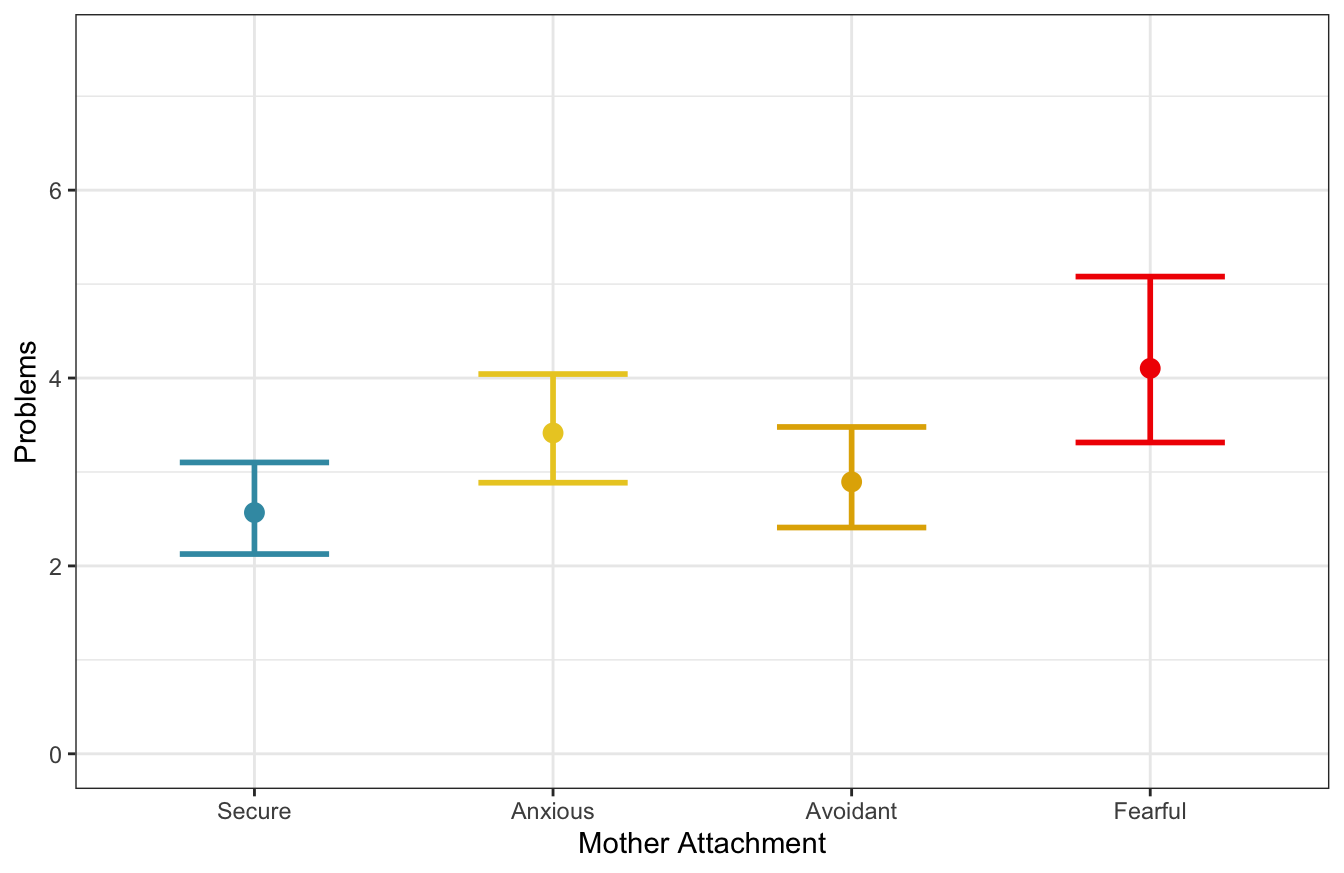
\includegraphics{attachment-bayes-factor_files/figure-latex/plot-comparison-effects-int-1} 

}

\caption{Marginal predicted values according to gender and mother attachment ($n_{subj} = 847$).}\label{fig:plot-comparison-effects-int}
\end{figure}

Post-hoc tests are run, considering pairwise comparisons and adjusting \emph{p}-values according to multivariate \emph{t}-distribution. Results are reported below,

\begin{Shaded}
\begin{Highlighting}[]
\NormalTok{emmeans}\SpecialCharTok{::}\FunctionTok{contrast}\NormalTok{(emmeans}\SpecialCharTok{::}\FunctionTok{emmeans}\NormalTok{(fit\_int\_mother, }\AttributeTok{specs =} \SpecialCharTok{\textasciitilde{}}\NormalTok{ mother ),}
                  \StringTok{"pairwise"}\NormalTok{, }\AttributeTok{adjust =} \StringTok{"mvt"}\NormalTok{)}
\DocumentationTok{\#\#  contrast           estimate     SE  df t.ratio p.value}
\DocumentationTok{\#\#  Secure {-} Anxious     {-}0.285 0.0892 837  {-}3.197  0.0079}
\DocumentationTok{\#\#  Secure {-} Avoidant    {-}0.120 0.0946 837  {-}1.266  0.5809}
\DocumentationTok{\#\#  Secure {-} Fearful     {-}0.469 0.1168 837  {-}4.011  0.0003}
\DocumentationTok{\#\#  Anxious {-} Avoidant    0.165 0.0869 837   1.903  0.2243}
\DocumentationTok{\#\#  Anxious {-} Fearful    {-}0.183 0.1096 837  {-}1.673  0.3346}
\DocumentationTok{\#\#  Avoidant {-} Fearful   {-}0.349 0.1167 837  {-}2.989  0.0149}
\DocumentationTok{\#\# }
\DocumentationTok{\#\# Results are averaged over the levels of: gender }
\DocumentationTok{\#\# Results are given on the log (not the response) scale. }
\DocumentationTok{\#\# P value adjustment: mvt method for 6 tests}
\end{Highlighting}
\end{Shaded}

Results indicate that Fearful and Anxious children have more problems than Secure children. Moreover, also the difference between Avoidant and Fearful children is significant.

To evaluate the fit of the model to the data, we computed the \emph{Marginal} \(R^2\) and the \emph{Conditional} \(R^2\).

\begin{Shaded}
\begin{Highlighting}[]
\NormalTok{performance}\SpecialCharTok{::}\FunctionTok{r2}\NormalTok{(fit\_int\_mother)}
\DocumentationTok{\#\# Warning: mu of 3.2 is too close to zero, estimate of random effect variances may be unreliable.}
\DocumentationTok{\#\# \# R2 for Mixed Models}
\DocumentationTok{\#\# }
\DocumentationTok{\#\#   Conditional R2: 0.209}
\DocumentationTok{\#\#      Marginal R2: 0.031}
\end{Highlighting}
\end{Shaded}

We can see that the actual variance explained by fixed effects is 3\%, not that much.

\hypertarget{conclusions-4}{%
\subsubsection*{Conclusions}\label{conclusions-4}}
\addcontentsline{toc}{subsubsection}{Conclusions}

Considering attachment theoretical perspectives, results indicate only the role of mother attachment so we can support the \textbf{Monotropy Theory}. Note, however, that the compared models contain no information regarding the expected direction of the effects but we only include/exclude predictors.

\hypertarget{BF-int}{%
\chapter{Bayes Factor}\label{BF-int}}

\hypertarget{encompassing-model-1}{%
\section{Encompassing Model}\label{encompassing-model-1}}

We define a Zero-Inflated Negative Binomial (ZINB) mixed-effects considering only the role of gender as a fixed effect and children's classroom ID as a random effect for \(p\). Whereas, regarding \(\mu\), we consider the interaction between mother and father attachment together with gender as fixed effects and children's classroom ID as a random effect. In the R formula syntax, we have

\begin{Shaded}
\begin{Highlighting}[]
\CommentTok{\# formula for p}
\NormalTok{p }\SpecialCharTok{\textasciitilde{}}\NormalTok{ gender }\SpecialCharTok{+}\NormalTok{ (}\DecValTok{1}\SpecialCharTok{|}\NormalTok{ID\_class)}

\CommentTok{\# formula for mu}
\NormalTok{mu }\SpecialCharTok{\textasciitilde{}}\NormalTok{ gender }\SpecialCharTok{+}\NormalTok{ mother }\SpecialCharTok{*}\NormalTok{ father }\SpecialCharTok{+}\NormalTok{ (}\DecValTok{1}\SpecialCharTok{|}\NormalTok{ID\_class)}
\end{Highlighting}
\end{Shaded}

\hypertarget{prior-choice-1}{%
\subsection{Prior Choice}\label{prior-choice-1}}

We set the same prior as for the externalizing problems analysis. The resulting prior settings are

\begin{verbatim}
##                   prior     class                          coef    group resp dpar nlpar lb ub       source
##            normal(0, 3)         b                                                                      user
##            normal(0, 3)         b                 fatherAnxious                                (vectorized)
##            normal(0, 3)         b                fatherAvoidant                                (vectorized)
##            normal(0, 3)         b                 fatherFearful                                (vectorized)
##            normal(0, 3)         b                       genderM                                (vectorized)
##            normal(0, 3)         b                 motherAnxious                                (vectorized)
##            normal(0, 3)         b   motherAnxious:fatherAnxious                                (vectorized)
##            normal(0, 3)         b  motherAnxious:fatherAvoidant                                (vectorized)
##            normal(0, 3)         b   motherAnxious:fatherFearful                                (vectorized)
##            normal(0, 3)         b                motherAvoidant                                (vectorized)
##            normal(0, 3)         b  motherAvoidant:fatherAnxious                                (vectorized)
##            normal(0, 3)         b motherAvoidant:fatherAvoidant                                (vectorized)
##            normal(0, 3)         b  motherAvoidant:fatherFearful                                (vectorized)
##            normal(0, 3)         b                 motherFearful                                (vectorized)
##            normal(0, 3)         b   motherFearful:fatherAnxious                                (vectorized)
##            normal(0, 3)         b  motherFearful:fatherAvoidant                                (vectorized)
##            normal(0, 3)         b   motherFearful:fatherFearful                                (vectorized)
##                  (flat)         b                                               zi                  default
##                  (flat)         b                       genderM                 zi             (vectorized)
##  student_t(3, 0.7, 2.5) Intercept                                                                   default
##          logistic(0, 1) Intercept                                               zi                  default
##    student_t(3, 0, 2.5)        sd                                                         0         default
##    student_t(3, 0, 2.5)        sd                                               zi        0         default
##    student_t(3, 0, 2.5)        sd                               ID_class                  0    (vectorized)
##    student_t(3, 0, 2.5)        sd                     Intercept ID_class                  0    (vectorized)
##    student_t(3, 0, 2.5)        sd                               ID_class        zi        0    (vectorized)
##    student_t(3, 0, 2.5)        sd                     Intercept ID_class        zi        0    (vectorized)
##       gamma(0.01, 0.01)     shape                                                         0         default
\end{verbatim}

\hypertarget{posterior-1}{%
\subsection{Posterior}\label{posterior-1}}

The encompassing model is estimated using 6 independent chains with 10,000 iterations (warm-up 2,000). Summary of the encompassing model is presented below.

\begin{verbatim}
##  Family: zero_inflated_negbinomial 
##   Links: mu = log; shape = identity; zi = logit 
## Formula: internalizing_sum ~ gender + mother * father + (1 | ID_class) 
##          zi ~ gender + (1 | ID_class)
##    Data: data (Number of observations: 847) 
##   Draws: 6 chains, each with iter = 10000; warmup = 2000; thin = 1;
##          total post-warmup draws = 48000
## 
## Group-Level Effects: 
## ~ID_class (Number of levels: 50) 
##                  Estimate Est.Error l-95% CI u-95% CI Rhat Bulk_ESS Tail_ESS
## sd(Intercept)        0.44      0.08     0.29     0.62 1.00     9576    21295
## sd(zi_Intercept)     2.24      0.55     1.38     3.53 1.00    23180    29061
## 
## Population-Level Effects: 
##                               Estimate Est.Error l-95% CI u-95% CI Rhat Bulk_ESS Tail_ESS
## Intercept                         0.83      0.13     0.57     1.08 1.00    20193    31209
## zi_Intercept                     -2.93      0.69    -4.54    -1.84 1.00    23885    24649
## genderM                           0.07      0.07    -0.07     0.22 1.00    69024    39479
## motherAnxious                     0.46      0.17     0.14     0.78 1.00    28713    34928
## motherAvoidant                   -0.08      0.25    -0.56     0.41 1.00    27088    33529
## motherFearful                     0.63      0.40    -0.13     1.44 1.00    25396    29183
## fatherAnxious                     0.07      0.17    -0.26     0.40 1.00    32754    37880
## fatherAvoidant                    0.08      0.18    -0.26     0.43 1.00    33099    33066
## fatherFearful                     0.36      0.34    -0.29     1.04 1.00    27438    31863
## motherAnxious:fatherAnxious      -0.24      0.23    -0.70     0.22 1.00    27476    35909
## motherAvoidant:fatherAnxious      0.24      0.31    -0.37     0.84 1.00    26127    33090
## motherFearful:fatherAnxious      -0.75      0.50    -1.75     0.22 1.00    27653    33582
## motherAnxious:fatherAvoidant     -0.23      0.24    -0.70     0.23 1.00    28023    34471
## motherAvoidant:fatherAvoidant     0.11      0.30    -0.48     0.70 1.00    24526    32104
## motherFearful:fatherAvoidant     -0.18      0.45    -1.10     0.68 1.00    25043    31079
## motherAnxious:fatherFearful      -0.46      0.40    -1.25     0.31 1.00    26068    32120
## motherAvoidant:fatherFearful      0.29      0.48    -0.66     1.22 1.00    26407    35222
## motherFearful:fatherFearful      -0.35      0.53    -1.41     0.67 1.00    22713    30152
## zi_genderM                       -0.31      0.41    -1.12     0.49 1.00    49631    32918
## 
## Family Specific Parameters: 
##       Estimate Est.Error l-95% CI u-95% CI Rhat Bulk_ESS Tail_ESS
## shape     2.47      0.32     1.90     3.17 1.00    36269    34308
## 
## Draws were sampled using sampling(NUTS). For each parameter, Bulk_ESS
## and Tail_ESS are effective sample size measures, and Rhat is the potential
## scale reduction factor on split chains (at convergence, Rhat = 1).
\end{verbatim}

\hypertarget{hypothesis-matrices-1}{%
\section{Hypothesis Matrices}\label{hypothesis-matrices-1}}

Hypothesis matrices are the same as in the analysis of the externalizing problems.

\hypertarget{centering-and-adjusting-1}{%
\section{Centering and Adjusting}\label{centering-and-adjusting-1}}

Centering and adjusting procedures are the same as in the analysis of the externalizing problems.

\hypertarget{results-and-sensitivity-1}{%
\section{Results and Sensitivity}\label{results-and-sensitivity-1}}

Bayes factor and posterior probability of each hypothesis are reported in Table\textasciitilde\ref{tab:table-bf-results-int}.

\begin{table}[!h]

\caption{\label{tab:table-bf-results-int}Bayes factor encompassing model and hypothesis posterior probabilities  ($n_{subj} = 847$).}
\centering
\begin{tabular}[t]{rcc>{\centering\arraybackslash}m{1cm}}
\toprule
\textbf{Hypothesis} & \textbf{Bayes Factor} & \textbf{Posterior Probability} & \textbf{ }\\
\midrule
Null & 3.4e+11 & 0.04 & 
\includegraphics[width=0.33in, height=0.33in]{images/ball_BF_int_null.png}\\
Monotropy & 8.8e+12 & 0.91 & 
\includegraphics[width=0.33in, height=0.33in]{images/ball_BF_int_monotropy.png}\\
Hierarchy & 4.8e+11 & 0.05 & 
\includegraphics[width=0.33in, height=0.33in]{images/ball_BF_int_hierarchy.png}\\
Independence & 1.1e+10 & 0.00 & 
\includegraphics[width=0.33in, height=0.33in]{images/ball_BF_int_independence.png}\\
Integration & 1.8e+10 & 0.00 & 
\includegraphics[width=0.33in, height=0.33in]{images/ball_BF_int_integration.png}\\
\bottomrule
\end{tabular}
\end{table}

Prior sensitivity analysis is conducted considering the same prior as in the analysis of the externalizing problems. The results of the prior sensitivity analysis are reported in Table\textasciitilde\ref{tab:table-sens-prior-analysis-int}.

\begin{table}[!h]

\caption{\label{tab:table-sens-prior-analysis-int}Bayes factor encompassing model and hypothesis posterior probabilities (PP) under different prior settings  ($n_{subj} = 847$).}
\centering
\resizebox{\linewidth}{!}{
\begin{tabular}[t]{>{}rcccrcccrcc}
\toprule
\multicolumn{1}{c}{\textbf{ }} & \multicolumn{2}{c}{\textbf{$\mathcal{N}(0, .5)$}} & \multicolumn{2}{c}{\textbf{$\mathcal{N}(0, 1)$}} & \multicolumn{2}{c}{\textbf{$\mathcal{N}(0, 3)$}} & \multicolumn{2}{c}{\textbf{$\mathcal{N}(0, 5)$}} & \multicolumn{2}{c}{\textbf{$\mathcal{N}(0, 10)$}} \\
\cmidrule(l{3pt}r{3pt}){2-3} \cmidrule(l{3pt}r{3pt}){4-5} \cmidrule(l{3pt}r{3pt}){6-7} \cmidrule(l{3pt}r{3pt}){8-9} \cmidrule(l{3pt}r{3pt}){10-11}
\textbf{Hypothesis} & \textbf{BF} & \textbf{PP} & \textbf{BF} & \textbf{PP} & \textbf{BF} & \textbf{PP} & \textbf{BF} & \textbf{PP} & \textbf{BF} & \textbf{PP}\\
\midrule
\textbf{Null} & 4.4e+01 & 0.00 & 8.4e+04 & 0.00 & 3.4e+11 & 0.04 & 6.8e+14 & 0.09 & 1.9e+19 & 0.27\\
\textbf{Monotropy} & 2.2e+04 & 0.28 & 1.9e+07 & 0.64 & 8.8e+12 & 0.91 & 6.5e+15 & 0.89 & 5.0e+19 & 0.72\\
\textbf{Hierarchy} & 4.0e+04 & 0.52 & 9.0e+06 & 0.29 & 4.8e+11 & 0.05 & 1.2e+14 & 0.02 & 2.2e+17 & 0.00\\
\textbf{Independence} & 5.8e+03 & 0.07 & 6.4e+05 & 0.02 & 1.1e+10 & 0.00 & 1.6e+12 & 0.00 & 1.6e+15 & 0.00\\
\textbf{Integration} & 1.0e+04 & 0.13 & 1.5e+06 & 0.05 & 1.8e+10 & 0.00 & 1.6e+12 & 0.00 & 8.2e+14 & 0.00\\
\bottomrule
\end{tabular}}
\end{table}

Overall results consistently indicate the Monotropy Hypothesis as the most supported by the data. However, we can observe the same patterns as in the analysis of the externalizing problems. More diffuse prior, favour hypothesis with more equality constraints. Whereas, tighter prior penalizes hypotheses with more equality constraints.

\hypertarget{selected-model-3}{%
\section{Selected Model}\label{selected-model-3}}

In the model, we consider only the role of gender and mother attachment as fixed effects of \(\mu\). In the R formula syntax, we have

\begin{Shaded}
\begin{Highlighting}[]
\CommentTok{\# formula for p}
\NormalTok{p }\SpecialCharTok{\textasciitilde{}}\NormalTok{ gender }\SpecialCharTok{+}\NormalTok{ (}\DecValTok{1}\SpecialCharTok{|}\NormalTok{ID\_class)}

\CommentTok{\# formula for mu}
\NormalTok{mu }\SpecialCharTok{\textasciitilde{}}\NormalTok{ gender }\SpecialCharTok{+}\NormalTok{ mother }\SpecialCharTok{+}\NormalTok{ (}\DecValTok{1}\SpecialCharTok{|}\NormalTok{ID\_class)}
\end{Highlighting}
\end{Shaded}

Again, we specify the same prior distributions as before. The resulting prior settings are

\begin{verbatim}
##                   prior     class           coef    group resp dpar nlpar lb ub       source
##            normal(0, 3)         b                                                       user
##            normal(0, 3)         b        genderM                                (vectorized)
##            normal(0, 3)         b  motherAnxious                                (vectorized)
##            normal(0, 3)         b motherAvoidant                                (vectorized)
##            normal(0, 3)         b  motherFearful                                (vectorized)
##                  (flat)         b                                zi                  default
##                  (flat)         b        genderM                 zi             (vectorized)
##  student_t(3, 0.7, 2.5) Intercept                                                    default
##          logistic(0, 1) Intercept                                zi                  default
##    student_t(3, 0, 2.5)        sd                                          0         default
##    student_t(3, 0, 2.5)        sd                                zi        0         default
##    student_t(3, 0, 2.5)        sd                ID_class                  0    (vectorized)
##    student_t(3, 0, 2.5)        sd      Intercept ID_class                  0    (vectorized)
##    student_t(3, 0, 2.5)        sd                ID_class        zi        0    (vectorized)
##    student_t(3, 0, 2.5)        sd      Intercept ID_class        zi        0    (vectorized)
##       gamma(0.01, 0.01)     shape                                          0         default
\end{verbatim}

The model is estimated using 6 independent chains with 6,000 iterations (warm-up 2,000). The model summary is presented below.

\begin{verbatim}
##  Family: zero_inflated_negbinomial 
##   Links: mu = log; shape = identity; zi = logit 
## Formula: internalizing_sum ~ gender + mother + (1 | ID_class) 
##          zi ~ gender + (1 | ID_class)
##    Data: data (Number of observations: 847) 
##   Draws: 6 chains, each with iter = 6000; warmup = 2000; thin = 1;
##          total post-warmup draws = 24000
## 
## Group-Level Effects: 
## ~ID_class (Number of levels: 50) 
##                  Estimate Est.Error l-95% CI u-95% CI Rhat Bulk_ESS Tail_ESS
## sd(Intercept)        0.43      0.08     0.29     0.61 1.00     4981    11555
## sd(zi_Intercept)     2.17      0.53     1.34     3.40 1.00    12787    16150
## 
## Population-Level Effects: 
##                Estimate Est.Error l-95% CI u-95% CI Rhat Bulk_ESS Tail_ESS
## Intercept          0.89      0.11     0.66     1.10 1.00    10532    14506
## zi_Intercept      -2.81      0.65    -4.31    -1.79 1.00    14230    13767
## genderM            0.07      0.07    -0.07     0.21 1.00    38142    19994
## motherAnxious      0.29      0.09     0.11     0.46 1.00    27686    19778
## motherAvoidant     0.12      0.10    -0.07     0.31 1.00    30305    18855
## motherFearful      0.48      0.12     0.25     0.71 1.00    28322    20529
## zi_genderM        -0.29      0.39    -1.07     0.48 1.00    27658    17214
## 
## Family Specific Parameters: 
##       Estimate Est.Error l-95% CI u-95% CI Rhat Bulk_ESS Tail_ESS
## shape     2.53      0.33     1.95     3.26 1.00    21194    18858
## 
## Draws were sampled using sampling(NUTS). For each parameter, Bulk_ESS
## and Tail_ESS are effective sample size measures, and Rhat is the potential
## scale reduction factor on split chains (at convergence, Rhat = 1).
\end{verbatim}

Marginal effects are presented in Figure\textasciitilde\ref{fig:plot-marginal-int} and differences between mother attachment patterns are reported in Figure\textasciitilde\ref{fig:plot-diff-int}.

\begin{figure}

{\centering 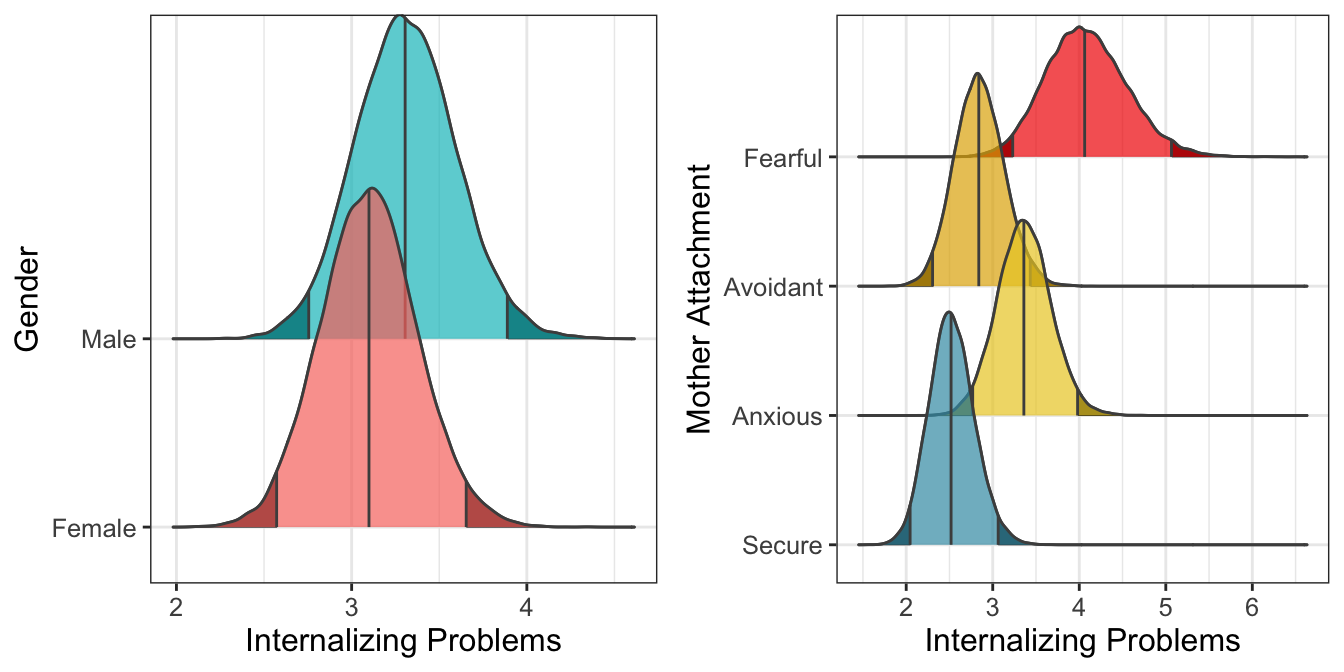
\includegraphics[width=0.95\linewidth]{attachment-bayes-factor_files/figure-latex/plot-marginal-int-1} 

}

\caption{Marginal predicted values according to gender and mother attachment ($n_{subj} = 847$).}\label{fig:plot-marginal-int}
\end{figure}

\begin{figure}

{\centering 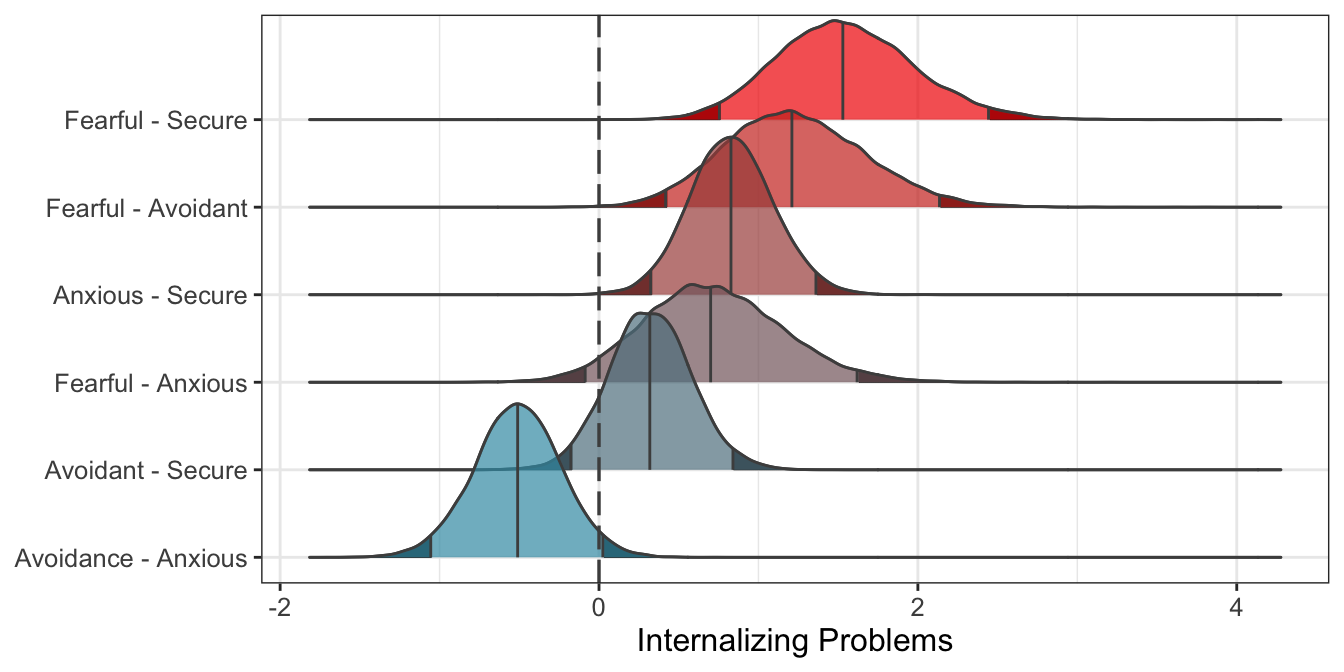
\includegraphics{attachment-bayes-factor_files/figure-latex/plot-diff-int-1} 

}

\caption{Predicted differences between mother attachment patterns ($n_{subj} = 847$).}\label{fig:plot-diff-int}
\end{figure}

Overall, results indicate that Fearful, and Anxious children have more problems than Secure children. Moreover, Fearful children have more problems than Avoidant children. Finally, also the difference between Avoidant and Anxious children is close to the threshold.

To evaluate the fit of the model to the data, we computed the \emph{Bayesian} \(R^2\) using the function \texttt{brms::bayes\_R2()}, and we present Posterior Predictions in Figure\textasciitilde\ref{fig:plot-ppcheck-int}.

\begin{Shaded}
\begin{Highlighting}[]
\NormalTok{r2\_int}
\DocumentationTok{\#\#     Estimate  Est.Error      Q2.5     Q97.5}
\DocumentationTok{\#\# R2 0.2224078 0.02975503 0.1660707 0.2825445}
\end{Highlighting}
\end{Shaded}

\begin{verbatim}
## Warning: Argument 'nsamples' is deprecated. Please use argument 'ndraws' instead.
\end{verbatim}

\begin{figure}

{\centering \includegraphics{attachment-bayes-factor_files/figure-latex/plot-ppcheck-int-1} 

}

\caption{Posterior predictive check ($n_{subj} = 847$).}\label{fig:plot-ppcheck-int}
\end{figure}

We can see that the actual variance explained by fixed effects and random effects is around 22\%. Moreover, the posterior predictive check indicates a good fit to the data.

\hypertarget{conclusions-5}{%
\subsubsection*{Conclusions}\label{conclusions-5}}
\addcontentsline{toc}{subsubsection}{Conclusions}

Considering attachment theoretical perspectives, results indicate only the role of mother attachment so we can support the Monotropy Theory.

\hypertarget{conclusion-int}{%
\chapter{Conclusions}\label{conclusion-int}}

Overall, we obtained consistent results from the three different approaches: only mother attachment influences children's externalizing problems. In particular, we observed the following pattern: Secure children have the lowest level of problems, Anxious and Avoidant children have a similar, intermediate, level of problems, and Fearful children have the highest level of problems. Compared to externalizing problems, however, differences between attachment groups are less pronounced. Taken together, these results support the Monotropy Theory.

  \bibliography{../Biblio-attachment.bib}

\end{document}
